\documentclass[12pt,letter]{article}
\usepackage{mathptmx} % added for time new roman font
\usepackage[left=1in,right=1in,top=1in,bottom=1in]{geometry}
\usepackage[latin1]{inputenc}
\usepackage{amsmath}
\usepackage[final]{pdfpages}
\usepackage{caption}	% added for \captionof
\usepackage[textsize=tiny]{todonotes}

% defines all example enviorment
\usepackage[framemethod=tikz]{mdframed} % added for the box around examples
\newtheorem{ex}{Example}
\numberwithin{ex}{section} % allows for the use of example numbers that lign up with the section numbers
\newenvironment{example}{\begin{mdframed}[middlelinewidth=0.5mm]\begin{ex}\normalfont}{\end{ex}\end{mdframed}}

% defines all review enviorment
\usepackage[framemethod=tikz]{mdframed} % added for the box around examples
\newtheorem{re}{Review}
\numberwithin{re}{section} % allows for the use of example numbers that lign up with the section numbers
\newenvironment{review}{\begin{mdframed}[middlelinewidth=2mm,roundcorner=20pt]\begin{re}\normalfont}{\end{re}\end{mdframed}}

% defines the quotation enviorment 
\usepackage{xcolor}
\newcommand{\quotebox}[2]{\begin{center}\fcolorbox{white}{blue!15!gray!15}{\begin{minipage}{0.9\linewidth}\vspace{10pt}\center\begin{minipage}{0.8\linewidth}{\space\Huge``}{#1}{\Huge''}{\break\null\hfill} {\small #2}  \end{minipage}\medbreak\end{minipage}}\end{center}}

% defines the definition enviorment 
\newcommand{\definitionbox}[2]{\begin{center}\fcolorbox{white}{blue!15!gray!15}{\begin{minipage}{0.9\linewidth}\vspace{10pt}\center\begin{minipage}{0.8\linewidth} {{\textbf{Definition} - }{#1}: {#2}}\end{minipage}\medbreak\end{minipage}}\end{center}}

\usepackage{amsfonts}
\usepackage{amssymb}
\usepackage{graphicx}
\usepackage{float}
\usepackage{booktabs}
%\usepackage{parskip} % remove all the paragraph indents
\usepackage{xfrac}
\usepackage{upgreek}
\usepackage{wrapfig}
\usepackage{setspace}
\usepackage[colorlinks=true]{hyperref}
\usepackage{textcomp} 
\usepackage{multicol} 
\usepackage{enumitem}		% added for spacing in itemize lists
\usepackage[numbered,framed]{matlab-prettifier}		% added for matlab code
\let\ph\mlplaceholder % shorter macro
\lstMakeShortInline"
\lstset{
  style              = Matlab-editor,
  basicstyle         = \mlttfamily,
  escapechar         = ",
  mlshowsectionrules = true,
}

\usepackage{color} % color added for editing
\newcommand{\bl}[1]{\textcolor[rgb]{0.00,0.00,1.00}{#1}}
\newcommand{\gr}[1]{\textcolor[rgb]{0.00,0.50,0.00}{#1}}
\newcommand{\rd}[1]{\textcolor[rgb]{0.75,0.00,0.00}{#1}}

\usepackage{fancyhdr}
\pagestyle{fancy}
\fancyfoot{} % clear all footer fields
\fancyfoot[R]{Page \thepage} 
%\fancyfoot[RE,LO]{Lecture notes developed for EMCH 516 at the University\\ of South Carolina. Wider distribution is not allowed. }

%%%%%%%		define the symbols for positive directions		%%%%%%
\makeatletter													%%	
																%%					
\newcommand*\curveplus{% positive counterclockwise				%%
  \mathbin{\rotatebox[origin=c]{90}{$\m@th\curvearrowleft$}+}}	%%
																%%
\newcommand*\rightplus{% positive right							%%
  \mathpalette\@rightplus\relax}								%%
\newcommand*\@rightplus[1]{%									%%
  \mathbin{\vcenter{\hbox{$\m@th\overset{#1+}{\to}$}}}}			%%
																%%	
\newcommand*\upplus{% positive up								%%
  \mathbin{+\mathord\uparrow}}									%%
																%%			
\newcommand*\downplus{% positive down							%%		
  \mathbin{+\mathord\downarrow}}								%%
  																%%		
\newcommand*\downrightplus{% positive down and right			%%	
  \mathbin{+ \rotatebox[origin=c]{-30}{$\m@th\rightarrow$}}}	%%
\makeatother 													%%	
%%%%%%%%%%%%%%%%%%%%%%%%%%%%%%%%%%%%%%%%%%%%%%%%%%%%%%%%%%%%%%%%%%


\usepackage{mathtools}          %loads amsmath as well added for the piece wise function
\DeclarePairedDelimiter\Floor\lfloor\rfloor
\DeclarePairedDelimiter\Ceil\lceil\rceil

 
\newcounter{NumberInTable}
\newcommand{\LTNUM}{\stepcounter{NumberInTable}{(\theNumberInTable)}}

\newcommand{\Laplace}[1]{\ensuremath{\mathcal{L}{\left[#1\right]}}}
\newcommand{\InvLap}[1]{\ensuremath{\mathcal{L}^{-1}{\left[#1\right]}}}
\renewcommand{\textuparrow}{$\uparrow$}

\usepackage{standalone} % This is the only new package required to compile the entire document
\usepackage{chapterbib}   

\numberwithin{equation}{section}	% added so the equsation numbers are section.# and start at section.1

\begin{document}

\begin{center}
	{\fontsize{50}{60}\selectfont Open Controls}
	
	\vspace{3cm}
	
	\begin{figure}[H]
		\includegraphics[width=6.5in]{figures/PID_controller.png}
		\label{fig:title_figure}
	\end{figure} 
	
	\vspace{3cm}
	
	\textbf{Austin R.J. Downey}\\ Department of Mechanical Engineering \\ Department of Civil and Environmental Engineering \\ University of South Carolina, Columbia SC, USA 
	
	\vspace{1.5cm}
	
	\textbf{Victor Giurgiutiu}\\  Department of Mechanical Engineering \\ University of South Carolina, Columbia SC, USA 
	
	\vspace{1cm}
	
	\today
\end{center}

\pagebreak

\section*{Preface}

This open-source text is designed to offer the reader a complete text on the basics of control theory within the contest of Mechanical Engineering. 


\subsection*{Cover Art}
A proportional-integral-derivative (PID) controller is a feed-back controller used in a variety of applications that require continuously modulated control. The Russian American engineer Nicolas Minorsky was arguably the first to develop the theoretical analysis of the PID controller in 1922  while he was researching and designing automatic ship steering for the US Navy. He based his work on watching how a ship's helmsman responds to wave loading on a ship, with a delayed input to the helm that not only considered the current ship course, but also past error and the desired rate of change for the ship. For a helmsman, the goal is stability, not absolute control, which simplifies how one thinks about the challenge of control.

\subsection*{License}
This work is licensed under a Creative Commons Attribution-ShareAlike 4.0 International License[cc-by-sa 4.0]. More information on the Attribution-ShareAlike 4.0 International (CC BY-SA 4.0) can be found at  \url{https://creativecommons.org/licenses/by-sa/4.0/}

\subsection*{Source Code}
The source code for this text is available at \url{https://github.com/austindowney/Open-Controls}.


\pagebreak

\tableofcontents

\pagebreak


%%%%%%%%%%%%%		Notes on compiling Document		%%%%%%%%%%%%%
% Notes on compiling Document
%
% 1. Each chapter can be compiled on there own.
% 2. I set the document up with a common figures folder to allow for the reuse of figures and generally to keep the document clean. 
% 3. When compiling the main document, you must include the \graphicspath{{xx}} for the first chapter, to set it in chapter 1. From here on, it will think its in the chapter one folder but the <../figures> in each folder will work with this. 
% 4. I (Austin Downey) have gotten this to compile on Windows with MikTeX and Linux with TeXLive. Your results may vary. For Linux, I:
% 	i.	added the extra {} in \graphicspath
% 	ii.	removed the .tex extension from the file names except for chapter 1. 
% 5. The common bibliography is an issue that has yet to be sorted out.
%%%%%%%%%%%%%%%%%%%%%%%%%%%%%%%%%%%%%%%%%%%%%%%%%%%%%%%%%%%%%%%%%%




% Chapter 1 Basic Concepts
\graphicspath{{Chapter_1_Basic_Concepts/}}
\documentclass[12pt,letter]{article}
\usepackage{mathptmx} % added for time new roman font
\usepackage[left=1in,right=1in,top=1in,bottom=1in]{geometry}
\usepackage[latin1]{inputenc}
\usepackage{amsmath}
\usepackage[final]{pdfpages}

\usepackage[textsize=tiny]{todonotes}

% defines all example enviorment
\usepackage[framemethod=tikz]{mdframed} % added for the box around examples
\newtheorem{ex}{Example}
\numberwithin{ex}{section} % allows for the use of example numbers that lign up with the section numbers
\newenvironment{example}{\begin{mdframed}[middlelinewidth=0.5mm]\begin{ex}\normalfont}{\end{ex}\end{mdframed}}

% defines all review enviorment
\usepackage[framemethod=tikz]{mdframed} % added for the box around examples
\newtheorem{re}{Review}
\numberwithin{re}{section} % allows for the use of example numbers that lign up with the section numbers
\newenvironment{review}{\begin{mdframed}[middlelinewidth=2mm,roundcorner=20pt]\begin{re}\normalfont}{\end{re}\end{mdframed}}

% defines the quotation enviorment 
\usepackage{xcolor}
\newcommand{\quotebox}[2]{\begin{center}\fcolorbox{white}{blue!15!gray!15}{\begin{minipage}{0.9\linewidth}\vspace{10pt}\center\begin{minipage}{0.8\linewidth}{\space\Huge``}{#1}{\Huge''}{\break\null\hfill} {\small #2}  \end{minipage}\medbreak\end{minipage}}\end{center}}

% defines the definition enviorment 
\newcommand{\definitionbox}[2]{\begin{center}\fcolorbox{white}{blue!15!gray!15}{\begin{minipage}{0.9\linewidth}\vspace{10pt}\center\begin{minipage}{0.8\linewidth} {{\textbf{Definition} - }{#1}: {#2}}\end{minipage}\medbreak\end{minipage}}\end{center}}

\usepackage{amsfonts}
\usepackage{amssymb}
\usepackage{graphicx}
\usepackage{float}
\usepackage{booktabs}
%\usepackage{parskip} % remove all the paragraph indents
\usepackage{xfrac}
\usepackage{upgreek}
\usepackage{wrapfig}
\usepackage{setspace}
\usepackage[colorlinks=true]{hyperref}
\usepackage{textcomp} 
\usepackage{multicol} 
\usepackage{enumitem}		% added for spacing in itemize lists
\usepackage[numbered,framed]{matlab-prettifier}		% added for matlab code
\let\ph\mlplaceholder % shorter macro
\lstMakeShortInline"
\lstset{
  style              = Matlab-editor,
  basicstyle         = \mlttfamily,
  escapechar         = ",
  mlshowsectionrules = true,
}

\usepackage{color} % color added for editing
\newcommand{\bl}[1]{\textcolor[rgb]{0.00,0.00,1.00}{#1}}
\newcommand{\gr}[1]{\textcolor[rgb]{0.00,0.50,0.00}{#1}}
\newcommand{\rd}[1]{\textcolor[rgb]{0.75,0.00,0.00}{#1}}

\usepackage{fancyhdr}
\pagestyle{fancy}
%\fancyfoot{} % clear all footer fields
%\fancyfoot[LE,RO]{Page \thepage} 

% Sets the footnotes to be letters, not numbers. This is needed or it's a mix of both. 
\renewcommand*\thefootnote{\alph{footnote}}

%%%%%%%		define the symbols for positive directions		%%%%%%
\makeatletter													%%	
																%%					
\newcommand*\curveplus{% positive counterclockwise				%%
  \mathbin{\rotatebox[origin=c]{90}{$\m@th\curvearrowleft$}+}}	%%
																%%
\newcommand*\rightplus{% positive right							%%
  \mathpalette\@rightplus\relax}								%%
\newcommand*\@rightplus[1]{%									%%
  \mathbin{\vcenter{\hbox{$\m@th\overset{#1+}{\to}$}}}}			%%
																%%	
\newcommand*\upplus{% positive up								%%
  \mathbin{+\mathord\uparrow}}									%%
																%%			
\newcommand*\downplus{% positive down							%%		
  \mathbin{+\mathord\downarrow}}								%%
  																%%		
\newcommand*\downrightplus{% positive down and right			%%	
  \mathbin{+ \rotatebox[origin=c]{-30}{$\m@th\rightarrow$}}}	%%
\makeatother 													%%	
%%%%%%%%%%%%%%%%%%%%%%%%%%%%%%%%%%%%%%%%%%%%%%%%%%%%%%%%%%%%%%%%%%


\usepackage{mathtools}          %loads amsmath as well added for the piece wise function
\DeclarePairedDelimiter\Floor\lfloor\rfloor
\DeclarePairedDelimiter\Ceil\lceil\rceil

 
\newcounter{NumberInTable}
\newcommand{\LTNUM}{\stepcounter{NumberInTable}{(\theNumberInTable)}}

\newcommand{\Laplace}[1]{\ensuremath{\mathcal{L}{\left[#1\right]}}}
\newcommand{\InvLap}[1]{\ensuremath{\mathcal{L}^{-1}{\left[#1\right]}}}
\renewcommand{\textuparrow}{$\uparrow$}

\numberwithin{equation}{section}	% added so the equsation numbers are section.# and start at section.1

\begin{document}
	
	% set the section number, along with figure and equation numbers
	\setcounter{section}{0}	
	\setcounter{figure}{0}   
	\renewcommand\thefigure{\thesection.\arabic{figure}}


\section{Text Overview}

\begin{itemize}
	\item Systems, 1\textsuperscript{st} order, 2\textsuperscript{nd} order, and higher order.
	\begin{itemize}
		\item Introduction to control systems		
		\item Differential equations
		\item General solution
		\item Free Response
		\item Stability 
		\item Laplace Transforms
	\end{itemize}
	\item Performance
	\begin{itemize}
		\item Time response
		\item Performance indicators
		\item System identification
	\end{itemize}
\item Control Systems
\begin{itemize}
	\item Feedback
	\item Stability
	\item Controllers 
\end{itemize}
\item Frequency Analysis
\begin{itemize}
	\item FRF
	\item Bode
	\item Nyquist
	\item Mangus 
\end{itemize}
\item Additional Topics
\begin{itemize}
	\item Combined Analysis
	\item CSD
	\item Single-input single-output (SISO)
	\item Tool
	\item State Space Models (introduction)
\end{itemize}

\end{itemize}



%		\begin{figure}[H]
%			\centering
%			\includegraphics[width=\linewidth]{../figures/simple_neural_network_vs_deep_learning.jpg}
%			\caption{simple neural network vs deep learning}
%			\label{fig:simple_neural_network_vs_deep_learning}
%		\end{figure}







\subsection{Basics of Control System}
A control system consisting of interconnected components is designed to achieve a desired purpose. To understand the purpose of a control system, it is useful to examine examples of control systems through the course of history. These early systems incorporated many of the same ideas of feedback that are in use today.

Modern control engineering practice includes the use of control design strategies for improving manufacturing processes, the efficiency of energy use, advanced automobile control, including rapid transit, among others. 



\noindent \textbf{System} - An interconnection of elements and devices for a desired purpose. \\


\noindent \textbf{Control System} - An interconnection of components forming a system configuration that will provide a desired response. \\

\noindent \textbf{Process} - The device, plant, or system under control. The input and output relationship represents the cause-and effect relationship of the process.


		\begin{figure}[H]
			\centering
			\includegraphics[]{../figures/control_system_input_output}
			\caption{Process to be controlled.}
			\label{fig:input_output_control_system}
		\end{figure}



\noindent \textbf{Open-Loop Control Systems} - utilize a controller or control actuator to obtain the desired response.


		\begin{figure}[H]
			\centering
			\includegraphics[]{../figures/control_system_open_loop}
			\caption{Open-loop control system (without feedback).}
			\label{fig:open_loop_control_system}
		\end{figure}

\noindent \textbf{Closed-Loop Control Systems} - utilizes feedback to compare the actual output to the desired output response.

		\begin{figure}[H]
			\centering
			\includegraphics[width=4.5in]{../figures/control_system_closed_loop}
			\caption{Closed-loop control system (with feedback).}
			\label{fig:closed_loop_control_system}
		\end{figure}



\noindent \textbf{Multivariable Control System} - a control system with multiple desired response controlled by multiple output variables. 


		\begin{figure}[H]
			\centering
			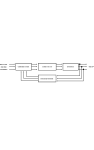
\includegraphics[width=4.5in]{../figures/control_system_closed_loop_multivariable}
			\caption{Multivariable control system with many inputs and many outputs to the system.}
			\label{fig:multivariable_control_system}
		\end{figure}


\noindent \textbf{Positive and negative feedback} - A positive feedback (also called Regenerative feedback) adds control outputs to the system in the same direction as the original perpetuation while a negative feedback (Degenerative feedback) provides a counteracting force to the original permutations.



\subsection{Videos of control systems}

\noindent \textbf{Ball and Plate PID control with 6 DOF Stewart platform}\\
\url{https://www.youtube.com/watch?v=j4OmVLc_oDw&t=95s&ab_channel=FullMotionDynamics}

\noindent \textbf{Ball and Plate PID control with 6 DOF Stewart platform}\\
\url{https://www.youtube.com/watch?v=meMWfva-Jio&ab_channel=StepanOzana}

\noindent \textbf{SpaceX first landing}\\
\url{https://www.youtube.com/watch?v=1sJlFzUQVmY&ab_channel=BloombergQuicktake}


\subsection{History}

\begin{itemize}
\item Greece (BC) - Float regulator mechanism.
\item Holland (16th Century) - Temperature regulator.
\item 18th Century James Watt's centrifugal governor for the speed control of a steam engine. 
\item 1920s Minorsky worked on automatic controllers for steering ships.
\item 1930s Nyquist developed a method for analyzing the stability of controlled systems.
\item 1940s Frequency response methods made it possible to design linear closed-loop control systems.
\item 1950s Root-locus method due to Evans was fully developed.
\item 1960s State space methods, optimal control, adaptive control.
\item 1980s Learning controls are begun to investigated and developed.
\item Present and on-going research fields. Recent application of modern control theory includes such non-engineering systems such as biological, biomedical, economic and socio-economic systems
\end{itemize}

\subsection{Examples of control systems}

Controllers in the form of centrifugal governors for steam engines set off the industrial revolution by allowing steam engines to produce reliable and controllable power. Figure~\ref{fig:steam_engines} shows centrifugal governor on steam engines. 

		\begin{figure}[H]
			\centering
			\includegraphics[]{../figures/steam_engines}
			\caption{Centrifugal governors on a: (a) Boulton \& Watt steam engine from 1788 \protect\footnotemark[1], and; (b) D. Napier \& Son from 1832 double-acting steam engine \protect\footnotemark[2].}
			\label{fig:steam_engines}
		\end{figure}
	\footnotetext[1]{Dr. Mirko Junge, CC BY 3.0 $<$https://creativecommons.org/licenses/by/3.0$>$, via Wikimedia Commons.}
	\footnotetext[2]{Nicol�s P�rez, CC BY-SA 3.0 $<$http://creativecommons.org/licenses/by-sa/3.0/$>$, via Wikimedia Commons.}

\pagebreak
		Arguably, the Russian American engineer Nicolas Minorsky was the first to develop the theoretical analysis for the three-term control we now call PID. This was done in 1922 while he was researching and designing automatic ship steering for the US Navy. He based his work on watching how a ship's helmsman responds to wave loading on a ship, with a delayed input to the helm that not only considered the current ship course, but also past error and the desired rate of change for the ship. For a helmsman, the goal is stability, not absolute control, which simplifies how one thinks about the challenge of control.

\begin{figure}[H]
	\centering
	\includegraphics[]{../figures/PID_Nicolas_Minorsky_and_USS_New_Mexico.png}
	\caption{Historical prospective of PID control showing: (a) Portrait of Nicolas Minorsky \protect\footnotemark[1] and (b) the battleship USS New Mexico (BB-40) of the United States Navy which was the first to implement PID control in its steering \protect\footnotemark[2]. }
	\label{fig:fragility_curve}
\end{figure}
	\footnotetext[1]{Peter Minorsky, grandson of Nicolas Minorsky, CC BY-SA 1.0 $<$https://creativecommons.org/licenses/by-sa/1.0$>$, via Wikimedia Commons} 
\footnotetext[2]{U.S. Navy, Public domain, via Wikimedia Commons} 



%\includepdf[pages=-,pagecommand={},width=0.9\textwidth]{PDF_notes/basics_of_control_system.pdf}
%
% \cite{Halevy2009UnreasonableEffectivenessData}
%
%
%
%	\pagebreak
%	\renewcommand{\thepage}{}
%	\renewcommand\refname{References Cited}
%	\pagestyle{plain}
%	\bibliographystyle{Downey_NSF}
%	\bibliography{Chapter_1_Basic_Concepts}


















\end{document}



% Chapter 2 systems
\documentclass[12pt,letter]{article}
\usepackage{mathptmx} % added for time new roman font
\usepackage[left=1in,right=1in,top=1in,bottom=1in]{geometry}
\usepackage[latin1]{inputenc}
\usepackage{amsmath}
\usepackage[final]{pdfpages}

\usepackage[textsize=tiny]{todonotes}

% defines all example enviorment
\usepackage[framemethod=tikz]{mdframed} % added for the box around examples
\newtheorem{ex}{Example}
\numberwithin{ex}{section} % allows for the use of example numbers that lign up with the section numbers
\newenvironment{example}{\begin{mdframed}[middlelinewidth=0.5mm]\begin{ex}\normalfont}{\end{ex}\end{mdframed}}

% defines all review enviorment
\usepackage[framemethod=tikz]{mdframed} % added for the box around examples
\newtheorem{re}{Review}
\numberwithin{re}{section} % allows for the use of example numbers that lign up with the section numbers
\newenvironment{review}{\begin{mdframed}[middlelinewidth=2mm,roundcorner=20pt]\begin{re}\normalfont}{\end{re}\end{mdframed}}

% defines the quotation enviorment 
\usepackage{xcolor}
\newcommand{\quotebox}[2]{\begin{center}\fcolorbox{white}{blue!15!gray!15}{\begin{minipage}{0.9\linewidth}\vspace{10pt}\center\begin{minipage}{0.8\linewidth}{\space\Huge``}{#1}{\Huge''}{\break\null\hfill} {\small #2}  \end{minipage}\medbreak\end{minipage}}\end{center}}

% defines the definition enviorment 
\newcommand{\definitionbox}[2]{\begin{center}\fcolorbox{white}{blue!15!gray!15}{\begin{minipage}{0.9\linewidth}\vspace{10pt}\center\begin{minipage}{0.8\linewidth} {{\textbf{Definition} - }{#1}: {#2}}\end{minipage}\medbreak\end{minipage}}\end{center}}

\usepackage{amsfonts}
\usepackage{amssymb}
\usepackage{graphicx}
\usepackage{float}
\usepackage{booktabs}
%\usepackage{parskip} % remove all the paragraph indents
\usepackage{xfrac}
\usepackage{upgreek}
\usepackage{wrapfig}
\usepackage{setspace}
\usepackage[colorlinks=true]{hyperref}
\usepackage{textcomp} 
\usepackage{multicol} 
\usepackage{enumitem}		% added for spacing in itemize lists
\usepackage[numbered,framed]{matlab-prettifier}		% added for matlab code
\let\ph\mlplaceholder % shorter macro
\lstMakeShortInline"
\lstset{
  style              = Matlab-editor,
  basicstyle         = \mlttfamily,
  escapechar         = ",
  mlshowsectionrules = true,
}

\usepackage{color} % color added for editing
\newcommand{\bl}[1]{\textcolor[rgb]{0.00,0.00,1.00}{#1}}
\newcommand{\gr}[1]{\textcolor[rgb]{0.00,0.50,0.00}{#1}}
\newcommand{\rd}[1]{\textcolor[rgb]{0.75,0.00,0.00}{#1}}

\usepackage{fancyhdr}
\pagestyle{fancy}
\fancyfoot{} % clear all footer fields
\fancyfoot[LE,RO]{Page \thepage} 
\fancyfoot[RE,LO]{}

%%%%%%%		define the symbols for positive directions		%%%%%%
\makeatletter													%%	
																%%					
\newcommand*\curveplus{% positive counterclockwise				%%
  \mathbin{\rotatebox[origin=c]{90}{$\m@th\curvearrowleft$}+}}	%%
																%%
\newcommand*\rightplus{% positive right							%%
  \mathpalette\@rightplus\relax}								%%
\newcommand*\@rightplus[1]{%									%%
  \mathbin{\vcenter{\hbox{$\m@th\overset{#1+}{\to}$}}}}			%%
																%%	
\newcommand*\upplus{% positive up								%%
  \mathbin{+\mathord\uparrow}}									%%
																%%			
\newcommand*\downplus{% positive down							%%		
  \mathbin{+\mathord\downarrow}}								%%
  																%%		
\newcommand*\downrightplus{% positive down and right			%%	
  \mathbin{+ \rotatebox[origin=c]{-30}{$\m@th\rightarrow$}}}	%%
\makeatother 													%%	
%%%%%%%%%%%%%%%%%%%%%%%%%%%%%%%%%%%%%%%%%%%%%%%%%%%%%%%%%%%%%%%%%%


\usepackage{mathtools}          %loads amsmath as well added for the piece wise function
\DeclarePairedDelimiter\Floor\lfloor\rfloor
\DeclarePairedDelimiter\Ceil\lceil\rceil

 
\newcounter{NumberInTable}
\newcommand{\LTNUM}{\stepcounter{NumberInTable}{(\theNumberInTable)}}

\newcommand{\Laplace}[1]{\ensuremath{\mathcal{L}{\left[#1\right]}}}
\newcommand{\InvLap}[1]{\ensuremath{\mathcal{L}^{-1}{\left[#1\right]}}}
\renewcommand{\textuparrow}{$\uparrow$}


\numberwithin{equation}{section}	% added so the equsation numbers are section.# and start at section.1

\begin{document}
	
	% set the section number, along with figure and equation numbers
	\setcounter{section}{1}	
	\setcounter{figure}{0}   
	\renewcommand\thefigure{\thesection.\arabic{figure}}


\section{Systems}

	\subsection{Basic Concepts in Vibrations}

    The study of vibrations, within the broader field of classical mechanics, is the investigation of oscillations that occur about an equilibrium point. Vibrations, both desired and undesired, are present in all mechanical systems and can be helpful (e.g. a soil sieve, rotary sander) or destructive (e.g. an aircraft frame in resonance). The oscillations that form a vibrating system may be periodic (e.g., pendulum) or random (e.g. turbulence in an airplane), or a combination of the two. 

    Vibrations impact our daily lives in a variety of ways, from the sound made by banjo strings that vibrates between 140 and 400 Hz to the 4-6 Hz vibration felt by a passenger in a car seat. The consideration of the vibrations and their associated mathematical modeling are an important factor in the design of mechanical systems. In the material that follows, the fundamental theories of vibration are presented and modeled using fundamental physical principles such and Newton's three laws of motion. These models and analyzed using the mathematical tools of calculus and differential equations. 

	\begin{review}
		Newton's three laws of motion:
		\begin{enumerate}
			\item In an inertial frame of reference, an object either remains at rest or continues to move at a constant velocity, unless acted upon by a force.
			\item In an inertial reference frame, the vector sum of the forces $F$ on an object is equal to the mass m of that object multiplied by the acceleration of the object: $F = ma$. (It is assumed here that the mass m is constant)
			\item When one body exerts a force on a second body, the second body simultaneously exerts a force equal in magnitude and opposite in direction on the first body.
		\end{enumerate}
	\end{review}

	\subsection{Single Degree-of-Freedom Systems}
	
        In its simplest form, the phenomenon of vibration is the exchange of energy between potential and kinetic energy. Therefore, a vibrating system must have a component that stores potential energy. This component must also be capable of releasing the energy as kinetic energy. This kinetic energy is stored in the movement of a mass where the measure of this movement is the velocity of the system and the continuous interchange between potential and kinetic energy is the vibration of the system. The simplest vibrating systems can be modeled as a single-degree-of-freedom (1-DOF) system. In a 1-DOF system, one variable can describe the motion of a system. Potential examples of  1-DOF systems include:
		
		\begin{enumerate}
			\item yo-yo
			\item pogo stick
			\item door swinging on axis
			\item throttle (gas pedal)
		\end{enumerate}
				
		\noindent Variables often used for describing 1-DOF systems are $x(t)$,  $y(t)$,  $z(t)$, and  $\theta(t)$.  Examples of 1-DOF systems are presented in figure \ref{fig:Examples_of_1DOF_systems} where the assumption of small displacements is made. Note: we will often drop the ``$(t)$'' for simplicity in this material. 

		\begin{figure}[H]
			\centering
			\includegraphics[]{../figures/Examples_of_1DOF_systems.png}
			\caption{Examples of single degree of freedom (DOF) systems showing: (a) a vertical spring-mass system; (b) a simple pendulum; and (c) a rotational spring-mass system.}
			\label{fig:Examples_of_1DOF_systems}
		\end{figure}

		\subsubsection{Spring-Mass Model}

			\quotebox{\Large{All models are wrong, but some are useful}}{George E.P. Box (1919 - 2013)}	
							
            Newtonian physics describes the motion of particles in terms of displacement $x$, velocity $\dot{x}$, and acceleration $\ddot{x}$ vectors. Moreover, from Newton's second law of motion says that the change in the velocity of mass in motion is a product of the force acting on the mass. A simple way to express this phenomenon is though a spring-mass model as presented in figure  \ref{fig:spring_mass_model_with_point_mass}. These spring-mass models neglect the mass of the spring and concentrate all the mass of the system into a single point. Note that in this case the force vector and mass-acceleration vectors lie on the same axis and as such are collinear. Therefore, these vectors can be easily treated as scalers simplifying the math used in the modeling of the system.     

			\begin{figure}[H]
				\centering
				\includegraphics[]{../figures/spring_mass_model_with_point_mass.png}
				\caption{A single-degree-of-freedom (1-DOF) spring mass model showing: (a) annotated schematic of a mass-spring system; and (b) the equivalent free-body diagram represented as a point-mass system.}
				\label{fig:spring_mass_model_with_point_mass}
			\end{figure}	
		
		\subsubsection{Linear Springs}
	
            Springs are mechanical devices that store energy, moreover, ideal spring is a theoretical representation of this mechanical device that is massless and responds with a linear increase in force for a unit increase in displacement (i.e. $F=kx$). For simplicity, the spring in the spring-mass model considered here is assumed aways ideal linear springs. A graphical representation of the idealized linear spring is presented in figure \ref{fig:linear_spring_deformation} where a unit force $F$ applied to the free end of the spring results in a unite displacement $x$ of the spring.  The resulting mathematical relationships,  $F=kx$, is known as Hooke's Law. Nonlinear springs add considerable complexity to the modeling of spring-mass systems, therefore, these are not considered in this introductory work. 
			
			\begin{figure}[H]
				\centering
				\includegraphics[]{../figures/linear_spring_deformation.png}
				\caption{Force-displacement plot for a linear spring.}
				\label{fig:linear_spring_deformation}
			\end{figure}					






					
	\subsubsection{Equation of Motion for an Oscillating System}			
			
        An Equation of Motion (EOM) is an equation that provides a basis for modeling a vibrating system about its equilibrium point and relates the transfer of the potential energy from the spring to the kinetic energy mass. In developing the EOM we assume that any surfaces are frictionless and as such, no energy is extracted from the vibrating system. Referencing the 1-DOF system in figure \ref{fig:EOM_1-DOF-mass_horizontal}(a), and assuming the mass only moves in the $x$ direction, the only force acting on the mass in the $x$ direction is the force that results from the elongation of the spring as annotated in figure \ref{fig:EOM_1-DOF-mass_horizontal}(b). Therefore, the sum of forces in along the $x$ axis must equal the mass ($m$) times the acceleration of the mass ($a\dot{x}$). 

		\begin{figure}[H]
			\centering
			\includegraphics[]{../figures/EOM_1-DOF-mass_horizontal.png}
			\caption{A spring mass model of a 1-DOF system showing: (a) a schematic of the system; (b)  free-body diagram of the system at its initial position.}
			\label{fig:EOM_1-DOF-mass_horizontal}
		\end{figure}			
		
		Considering that positive displacements are to the right, the standard form of the equation of motion for an undamped system without any excitation is expressed as:  
		\begin{equation}
			s_1 \ddot{x} + s_2 x = 0
		\end{equation}			
		where $s_1$ and $s_2$ are constants to be determined for the specific system. A systematic approach to obtaining free-body diagram (FBD) of a system under vibration can be expressed in three steps:
		\begin{enumerate}
			\item Draw a free-body diagram (FBD) at the system's equilibrium and displaced position (without a displacing force).
			\item Apply Newton's second law to both FBDs ( equilibrium and displaced).
			\item Combine the equations to write the EOM in standard form with the forcing component on the right-hand side. For free vibration, the forcing component is 0. 
		\end{enumerate}
			
		Solving these three steps for 1-DOF system presented in figure \ref{fig:EOM_1-DOF-mass_horizontal} results in the EOM:
		\begin{equation}
			m \ddot{x} + k x = 0
		\end{equation}

		\begin{review}
			A second-order linear homogeneous differential equation has the form:
			
			\begin{equation}
			 a \ddot{x} + b \dot{x} + cx = 0
			\end{equation}
		
			\noindent The EOM for a 1-DOF system under a free vibration is a a second-order differential equation due to acceleration ($\ddot{x}$) being the second derivative of displacement ($x$) and homogeneous as the forcing function (right-hand side of the equations) is zero. In EOM's current form, $m=k$, $b=0$,  and $c=k$. In future work, $b$ will account for damping in the vibrating system.     
		\end{review}

					
		\begin{example}			
			
			Considering the system:
			\begin{figure}[H]
				\centering
				\includegraphics[]{../figures/1-DOF-spring_mass_horizontal.png}
			\end{figure}		
			
			\textbf{Step-1}
			Define the direction of displacement, and draw the FBD for the equilibrium and displaced state.  
			\begin{figure}[H]
				\centering
				\includegraphics[width=0.45\textwidth]{../figures/1-DOF-mass_horizontal_FBD.png}\\
				equilibrium state \hspace{3cm} displaced state
			\end{figure}		
			\noindent The equation for the equilibrium state is:
			\begin{equation}
			\rightplus \sum F_x = 0
			\end{equation}
			and in the displaced state:
			\begin{equation}
			\rightplus \sum F_x = -kx
			\end{equation}		
			This equation does not equal zero as the FBD does not account for the restoring force. 
	
			\noindent	\textbf{Step-2} Apply Newton's second law (we want to store energy in the kinetic state) of motion to the sum of forces for the displaced position we get: 		 		
			\begin{equation}
			ma = m\ddot{x} = \rightplus \sum F_x = -kx
			\end{equation}			
			\begin{equation}
			m\ddot{x} = -kx
			\end{equation}				
			\textbf{Step-3} Rearrange in the Equation to construct an EOM: 			
			\begin{equation}
			m\ddot{x} + kx = 0
			\end{equation}		
		\end{example}			

		\begin{example}	
			Some systems will have an initial displacement, as the system will oscillate around this position we need to define the EOM about this position. Considering the system:
			\begin{figure}[H]
				\centering
				\includegraphics[]{../figures/1-DOF-spring_mass_vertical.png}
			\end{figure}		
			\noindent \textbf{Step-1}
			Define the direction of displacement, and draw the FBD for the equilibrium and displaced state.  
			\begin{figure}[H]
				\centering
				\includegraphics[]{../figures/1-DOF-spring_mass_vertical_FBD.png}\\
				equilibrium state \hspace{3cm} displaced state
			\end{figure}		
			\noindent The equation for the equilibrium state is:
			\begin{equation}
				\downplus \sum F_x = mg - k\delta = 0
			\end{equation}
			and in the displaced state:
			\begin{equation}
				\downplus \sum F_x =mg -k(\delta + x)
			\end{equation}	
			This equation does not equal zero as the FBD does not account for the restoring force.	
			
			\noindent \textbf{Step-2} Apply Newton's second law (we want to store energy in the kinetic state) of motion to the sum of forces for the displaced position we get: 		
			\begin{equation}
				m\ddot{x} = \downplus \sum F_x =mg -k\delta -kx
			\end{equation}
			We can than use the information from the equilibrium state to cancel out some terms, this becomes:
			\begin{equation}
				m\ddot{x} = -kx
			\end{equation}				
			\textbf{Step-3} Rearrange in the Equation to construct an EOM: 					
			\begin{equation}
				m\ddot{x} + kx = 0
			\end{equation}			
		\end{example}	




\subsection{Forcing Function}

\subsubsection{Step Function}

A step function is a common loading situation and can represent the dropping of a load into a truck, a car going over a curve, or a motor starting up. The step function ($\Phi$) is also know as the Heaviside function

\begin{figure}[H]
	\centering
	\includegraphics[width=6.5in]{../figures/step.png}
	\caption{Step function.}
\end{figure}



\subsubsection{Pulse Function}

Pulse function ($\rho(t;\uptau)$) consists of a step up at $t=0$ followed by a step down at $t=\uptau$. The amplitude is $\sfrac{1}{\uptau}$ so that the area under the pulse is constant and equal to unity ($A=1$). 

\begin{figure}[H]
	\centering
	\includegraphics[width=5.5in]{../figures/pulse_function.png}
	\caption{Pulse function.}
\end{figure}

\subsubsection{Impulse Function}

Shock loads on mechanical systems represent a very common source of vibration. These short-duration forces are also called called an impulse. An impulse excitation is defined as a force that is applied for a very short, or infinitesimal, length of time. An impulse is a nonperiodic force that is represented by the symbol $\delta$. Impulse function ($\delta(t)$) is also known as the ``Dirac function'', ``Dirac delta function'', ``Dirac impulse function'', or ``delta function''. The impulse function $\delta(t)$ is obtained from the pulse function $\rho(t;\uptau)$ by letting $\uptau$ become infinitesimally small, i.e., 

\begin{figure}[H]
	\centering
	\includegraphics[width=5.5in]{../figures/impulse_function.png}
	\caption{Impulse function.}
\end{figure}

The area under the $delta$ function is equal to unity ($A=1$) just like the pulse function $\rho(t;\uptau)$.

\subsubsection{Ramp Function}

The ramp function is zero for $t<0$ and equal to $t$ for $t>0$. 

\begin{figure}[H]
	\centering
	\includegraphics[width=3.5in]{../figures/ramp_function.png}
	\caption{Ramp function.}
\end{figure}



	\subsection{Introduction to Stability}

	The stability of a system is explained though ``poles'' and ``zeros''. The poles and the zeros of a system determine whether the system is stable, and how well the system performs.

	\begin{enumerate}
		\item A system at a pole has an output that is infinite even though the input to the system was finite (i.e. unstable). 
		\item A system at a zero has an output that is finite even though the input to the system was infinite (i.e. stable).
	\end{enumerate}
 








			\begin{figure}[H]
				\centering
				\includegraphics[width=5.0in]{../figures/transfer_function_poles_and_zeros_and_3D_space.png}
				\caption{Poles and zeros.}
				\label{fig:transfer_function_poles_and_zeros_and_3D_space}
			\end{figure}

	Control systems can be designed simply by assigning specific values to the poles and zeros of the system. Physically realizable control systems must have a number of poles greater than the number of zeros. Systems that satisfy this relationship are called Proper. For a rational polynomial transfer function: The poles of a transfer function are defined as the roots of the denominator polynomial of the transfer function.  The zeros of a transfer function are simply the roots of the numerator polynomial. Visualizing of poles and zeros in the complex space can be helpful in understanding the stability of the system. Figure~\ref{fig:transfer_function_poles_and_zeros_and_3D_space} shows the complex space for an arbitrary transfer function $\sfrac{(s+2)(s-3)}{s^2+4s+20}$ where figure~\ref{fig:transfer_function_poles_and_zeros_and_3D_space}(a) shows the 3D space while figure~\ref{fig:transfer_function_poles_and_zeros_and_3D_space}(b) just reports the poles and zeros of the transfer function.  Figure~\ref{fig:transfer_function_3D_space_3_examples} reports the transfer functions for 3 additional transfer functions.  

			\begin{figure}[H]
				\centering
				\includegraphics[width=6.5in]{../figures/transfer_function_3D_space_3_examples.png}
				\caption{Poles and zeros in the complex space, plotted for 3 transfer functions.}
				\label{fig:transfer_function_3D_space_3_examples}
			\end{figure}





	\subsection{1\textsuperscript{st} Order Systems}	




	\subsubsection{Spring-damper mechanism}


Consider the system:
\begin{figure}[H]
	\centering
	\includegraphics[]{../figures/1-DOF-spring_dashpot_horizontal_forced_FBD.png}
	\caption{Damped 1-DOF system with an external force ($F(t)$) applied, showing: (a) the system configuration; and (b) the free body diagram}
\end{figure}	
Making the assumption that this system does not have any mass, the force balance equation is written as: 
\begin{equation}
-kx - c\dot{x} + f^* =0
\end{equation}
this becomes the equation of motion
\begin{equation}
c\dot{x} + kx = f^*
\end{equation}
normalizing the equation of motion by the stiffness $k$, 
\begin{equation}
\frac{c}{k}\dot{x} + x = \frac{1}{k}f^*
\end{equation}
define the \emph{time constant} $T$ as 
\begin{equation}
T=\frac{c}{k}
\end{equation}
and the normalized forcing function $f(t) = \frac{1}{k}f^*(t)$. This results in the 1\textsuperscript{st}-order ODE in standard form:
\begin{equation}
T\dot{x}(t) + x(t) = f(t)
\label{eq:ODE}
\end{equation}
A general solution for this ODE is written as:
\begin{equation}
x(t) = x_\text{c}(t)+x_\text{p}(t)
\label{eq:ODE_solution}
\end{equation}
where: $x_\text{c}$ is called the ``complementary solution'' and satisfies the homogeneous equation and satisfies the homogeneous equation 
\begin{equation}
T\dot{x}_\text{c} + x_\text{c} = 0
\end{equation}
The homogeneous equation is obtained from equation~\ref{eq:ODE} by making zero the right had side.  The complementary solution $x_\text{c}$ is the free response.

$x_\text{p}(t)$  is called the ``particular solution'' and is used to satisfy the right-hand side of equation~\ref{eq:ODE}. Substituting equation~\ref{eq:ODE_solution} into equation~\ref{eq:ODE} yields:

\begin{equation}
T(\dot{x}_\text{c} + \dot{x}_\text{p}) + x_\text{c}+x_\text{p} = f(t)
\end{equation}
or
\begin{equation}
T\dot{x}_\text{c} + x_\text{c} + T \dot{x}_\text{p} + x_\text{p} = f(t)
\end{equation}
As $T\dot{x}_\text{c} + x_\text{c}=0$:
\begin{equation}
T \dot{x}_\text{p} + x_\text{p} = f(t)
\end{equation}
This shows that:
\begin{itemize}
\item $T\dot{x}_\text{c} + x_\text{c}$ is the solution to the free response.
\item $T \dot{x}_\text{p} + x_\text{p}$ is the solution to the forced response.
\end{itemize}

\subsubsection{Homogeneous Equation (Free Response)}

The Homogeneous equation is obtained from equation~\ref{eq:ODE} and setting the right had side to zero:
\begin{equation}
T\dot{x}_\text{c} + x_\text{c} = 0
\label{eq:homogenous_solution}
\end{equation}
To solve, assume: \todo{I really think $c$ should be $a$ or it confuses with damping.}
\begin{align}
\label{eq:lambda}
x_\text{c}(t) &= c e^{ p t} \\
\dot{x}_\text{c}(t) &= p c e^{ p t} \nonumber
\end{align}
Inserting equation~\ref{eq:lambda} into equation~\ref{eq:homogenous_solution} gives:
\begin{equation}
T (p c e^{ p t}) + c e^{ p t} = 0
\end{equation}
canceling out like terms results in the ``characteristic equation'':
\begin{equation}
T p  + 1 = 0
\label{eq:characteristic_equation}
\end{equation}
therefore:
\begin{equation}
p  = \frac{-1}{T}
\label{eq:pole}
\end{equation}
where this is a ``pole'' of the system. Inserting equation~\ref{eq:pole} into equation~\ref{eq:lambda} results in the ``free response'' of the system:
\begin{equation}
\label{eq:free_response}
x_\text{c}(t) = c e^{ \sfrac{-t}{T}}
\end{equation}
as shown in figure~\ref{fig:1-DOF_free_decay}. Note that the lack of mass in the system prevents it from oscillate as there is no way for it to hold kinetic energy, and therefore no way for it to exchange energy between potential and kinetic forms. 
\begin{figure}[H]
	\centering
	\includegraphics[width=4in]{../figures/free_decay.png}
	\caption{Free decay of a 1-DOF system}
	\label{fig:1-DOF_free_decay}
\end{figure}

\subsubsection{Stability of 1\textsuperscript{st}-order systems}
Using the general free response form eq~\ref{eq:free_response} where $p$ is a root of the charismatic equation (equation~\ref{eq:characteristic_equation}) and is called the ``pole''. The stability of the system is dictate by the sing of of $p$, i.e., its location in the complex $p$ plane.

\begin{mdframed}[middlelinewidth=0.5mm]
\begin{center}
\bl{NOTE}
\end{center}
A \textbf{Stable System} is a system where if a disturbance is applied, then the system returns to its initial state. 
\end{mdframed}

\begin{figure}[H]
	\centering
	\includegraphics[width=6.5in]{../figures/system_stability_first_order.png}
	\caption{Stability of a first order system for different $p$ values.}
\end{figure}


\subsubsection{Stability of 1\textsuperscript{st}-order Systems Under Forced Response}


The total solution of equation~\ref{eq:ODE} is given as:
\begin{equation}
x(t) = x_\text{c}(t)+x_\text{p}(t)
\end{equation}
or as:
\begin{equation}
x(t) = c e^{ \sfrac{-t}{T}} + x_\text{p}(t)
\end{equation}
The constant $c$ and the function $x_\text{p}(t)$ have to be determined depending on initial conditions and the forms of $f(t)$. In control theory, the initial conditions are usually assumed go be zero. 

\todo{This is incomplete and needs more context.}



\subsection{2\textsuperscript{nd} Order Systems}


Consider the system:
			\begin{figure}[H]
				\centering
				\includegraphics[]{../figures/1-DOF-spring_mass_horizontal_forced_FBD.png}
				\caption{1-DOF system with an external force ($F(t)$) applied, showing: (a) the system configuration; and (b) the free body diagram}
				\label{fig:1-DOF-spring_mass_horizontal_forced_FBD}
			\end{figure}	

Newton's second law of motion states:
\begin{equation}
m \ddot{x} = -k + f^*
\end{equation}
this can be rearranged to the standard equation of motion for a system with forced vibrations:
\begin{equation}
m \ddot{x}(t) + kx(t) = f^*
\label{eq:EOM_2nd}
\end{equation}
It is an 2\textsuperscript{nd}-order inhomogeneous ordinary differential equation in time $t$.  Similar to the solutions to the EOM for a 1\textsuperscript{st}-order system, the solution for a 2\textsuperscript{nd}-order system ae made of two parts, the ``complementary solution'' and the ``particular solution''. Again, this is written as:
\begin{equation}
x(t) = x_\text{c}(t)+x_\text{p}(t)
\end{equation}
where $x_\text{c}(t)$ satisfies the homogeneous equation ($m \ddot{x}(t) + kx(t) = 0$) and represent the ``free'' response of the system. $x_\text{p}(t)$ satisfies the complete equation $m \ddot{x}(t) + kx(t) = f^*$ and represents the ``forced'' response of the system.


\subsubsection{Homogeneous Equation (Free Vibration Response)}

The homogeneous equation $x_\text{c}(t)$ is obtained by setting the forcing function of the EOM to zero:
\begin{equation}
m \ddot{x}(t) + kx(t) = 0
\end{equation}
normalizing by the mass returns:
\begin{equation}
\ddot{x}(t) + \frac{k}{m}x(t) = 0
\end{equation}
denoting the natural frequency of the system:
\begin{equation}
\omega_\text{n}^2 = \frac{k}{m}
\end{equation}
or more simply (and traditionally)
\begin{equation}
\omega_\text{n} = \sqrt{\frac{k}{m}}
\end{equation}
Inserting the natural frequency of the system back into the EOM yields the homogeneous equation in standard form:
\begin{equation}
\ddot{x} + \omega_\text{n}^2 x = 0
\end{equation}
To solve the homogeneous equation, assume the form:
\begin{equation}
x\text(t) = c e^{ p t} 
\end{equation}
hence
\begin{align}
\dot{x}(t)&= p c e^{ p t}  = px\\
\ddot{x}(t)&= p^2 c e^{ p t} = p^2x \nonumber
\end{align}
inserting these back into the EOM for the 2\textsuperscript{nd}-order system results in:
\begin{equation}
 p^2x + \omega_\text{n}^2 x = 0
\end{equation}
this simplifies to the characteristic equation:
\begin{equation}
 p^2 + \omega_\text{n}^2 = 0
\end{equation}
Rearranging this equations lead to
\begin{equation}
 p^2  = -\omega_\text{n}^2
\end{equation}
and considering that $i=\sqrt{-1}$ to the solution
\begin{equation}
p_{1,2}  = \pm i \omega_\text{n}
\end{equation}
inserting these back into the EOM for the 2\textsuperscript{nd}-order system results in:
\begin{equation}
x_\text{c}(t) = c_1 e ^{i \omega_\text{n} t} + c_2 e ^{-i \omega_\text{n} t} 
\end{equation}
which is the the complementary solution where $c_1$ and $c_2$ are constants to be determine.  The complementary solution can also be written as:
\begin{equation}
x_c(t) = c \sin(\omega_\text{n} t + \phi) 
\end{equation}
where $c$ is the amplitude of oscillation and $\phi$ is the phase angle. 

\begin{figure}[H]
	\centering
	\includegraphics[]{../figures/harmonic_motion_2.png}
	\caption{Summary of the temporal response for a 1-DOF system.}
	\label{fig:Harmonic_Motion_2.png}
\end{figure}
\noindent where $x_0$ and $v_0$ are the is the displacement and velocity at $t$=0 (i.e. the initial displacement). 

		\begin{review}
		
			Euler's (pronounced oy-ler) formula, named after Swiss engineer and mathematician Leonhard Euler (1707-1783), is a mathematical formula in complex analysis that establishes the fundamental relationship between the trigonometric functions and the complex exponential function. Euler's formula states that for any real number $x$,
			\begin{equation}
				e^{j\psi} = \text{cos}(\psi) + j \text{sin}(\psi)
			\end{equation}		
			where $j=\sqrt{-1}$. This equation can also be expressed as:
			\begin{equation}
				e^{-j\psi} = \text{cos}(\psi) - j \text{sin}(\psi)
			\end{equation}	
			This can be expressed in terms of polar coordinates as:				
			\begin{figure}[H]
				\centering
				\includegraphics[]{../figures/Eulers_formula.png}
				\caption{Euler's formula illustrated on the unit circle in the complex plane.}
			\end{figure}
		\end{review}


\begin{mdframed}[middlelinewidth=0.5mm]
\begin{center}
\gr{Proof}
\end{center}
Showing that $x_\text{c}(t) = c_1 e ^{i \omega_\text{n} t} + c_2 e ^{-i \omega_\text{n} t} $ is the same as $x_c(t) = C \sin(\omega_\text{n} t + \phi) $, consider Euler's identity, 
\begin{equation}
e^{i \alpha} = \cos(\alpha) + i \sin(\alpha)
\end{equation}
therefore:
\begin{align}
c_1 e ^{i \omega_\text{n} t}   &= c_1 \cos(\omega_\text{n} t) + c_1 i \sin(\omega_\text{n} t)  \\
c_2 e ^{- i \omega_\text{n} t}   &= c_2 \cos(\omega_\text{n} t) + c_2 i \sin(\omega_\text{n} t)   \nonumber
\end{align}
rearranging terms yields:
\begin{equation}
c_1 e ^{i \omega_\text{n} t} + c_2 e ^{- i \omega_\text{n} t}  = (c_1+c_2) \cos(\omega_\text{n} t) + (c_1+c_2) i \sin(\omega_\text{n} t) 
\end{equation}
which is equivalent to:
\begin{equation}
c_1 e ^{i \omega_\text{n} t} + c_2 e ^{- i \omega_\text{n} t}  = A \cos(\omega_\text{n} t) + B \sin(\omega_\text{n} t) 
\end{equation}
where:
\begin{equation}
A = c_1 + c_2; \;\; B = i(c_1 - c_2)
\end{equation}


Recall that $\sin(\alpha + \beta) = \sin(\alpha) \cos(\beta) + \cos(\alpha) \sin(\beta)$. Therefore, $x_c(t) = c \sin(\omega_\text{n} t + \phi)$ can be written as (with a little rearranging):
\begin{equation}
x_\text{c}(t) = c \cos(\phi) \sin(\omega_\text{n} t) + c \sin(\phi) \cos(\omega_\text{n} t)
\end{equation}
Therefore we can show that: 
\begin{equation}
A \cos(\omega_\text{n} t) + B \sin(\omega_\text{n} t) = c \sin(\omega_\text{n} t + \phi) 
\end{equation}
as
\begin{equation}
B = c\cos(\phi); \;\; A = c\sin(\phi)
\end{equation}
Moreover, 
\begin{equation}
A^2 + B^2 = C^2 \sin^2(\phi) + C^2 \cos^2(\phi) = C^2 \big(  \sin^2(\phi) + \cos^2(\phi)\big) = C^2
\end{equation}
and 
\begin{equation}
C = \sqrt{A^2 + B^2}, \;\;\;\;  \frac{A}{B} = \frac{c \sin(\phi)}{c \cos(\phi)} = c \tan(\phi), \;\;\;\;  \phi = \tan^{-1} \frac{A}{B}
\end{equation}

\end{mdframed}

The Standard form of Inhomogeneous Equation can be found, starting at the EOM:
\begin{equation}
m \ddot{x} + kx = f^*
\end{equation}
divide by $m$, therefore:
\begin{equation}
\ddot{x} + \frac{k}{m}x = \frac{1}{m}f^*
\end{equation}
Recall that $\frac{k}{m} = \omega_\text{n}^2$ and define the normalized forcing function as $f(t) = \frac{1}{k}f^*$, this results in:
\begin{equation}
\frac{1}{m}f^*(t) = \frac{1}{m}kf(t) = \omega_\text{n}^2 f(t)
\end{equation}
inserting this back into the the EOM yields a 2\textsuperscript{nd}-order inhomogeneous ODE in standard form:
\begin{equation}
\ddot{x} + \frac{k}{m}x = \omega_\text{n}^2 f(t)
\label{eq:ODE_2_standard}
\end{equation}


\subsection{Forced Vibration Response}

The total vibration $x(t)$ of the system can be explained as:
\begin{equation}
x(t) = x_\text{c}(t) + x_\text{p}(t) = C \sin(\omega_\text{n}t + \phi) + x_\text{p}(t)
\end{equation}
inserting the first part of this expression for $x(t)$ into equation~\ref{eq:ODE_2_standard} yields:
\begin{equation}
\ddot{x}_\text{c} + \ddot{x}_\text{p} + \omega_\text{n}^2(x_\text{c} + x_\text{p}) = \omega_\text{n}^2 f(t)
\end{equation}
assuming that the complementary solution equals zero, this expression simplifies to:
\begin{equation}
\ddot{x}_\text{p} + \omega_\text{n}^2x_\text{p} = \omega_\text{n}^2 f(t)
\end{equation}
This expressions requires that we find $c$, $\phi$, and $x_\text{p}(t)$; this is not easy. 

\subsection{Spring-mass-damper oscillator}

Consider the system:
\begin{figure}[H]
	\centering
	\includegraphics[]{../figures/1-DOF-spring_dashpot_mass_horizontal_forced_FBD.png}
	\caption{Damped 1-DOF system with an external force ($F(t)$) applied, showing: (a) the system configuration; and (b) the free body diagram}
\end{figure}
Newtons second law of motion tells us
\begin{equation}
m \ddot{x} = -kx - c\dot{x} + f^*
\end{equation}
therefore, we can write the EOM as:
\begin{equation}
m \ddot{x}(t) + c\dot{x}(t) + kx(t) = f^*(t)
\label{eq:EOM_2nd_forced}
\end{equation}
for the considered damped forced vibration problem. This is a 2\textsuperscript{nd} order inhomogeneous ODE. As before, the solution of $x(t)$ for equation~\ref{eq:EOM_2nd_forced} is the sum of the complementary and particular solution where the complementary solution satisfies the homogeneous equation while the particular solution satisfies the inhomogeneous equation. 

To solve the homogeneous equation, set the right hand side of equation~\ref{eq:EOM_2nd_forced} to zero to get the equation for damped free vibration:
\begin{equation}
m \ddot{x}(t) + c\dot{x}(t) + kx(t) = 0
\end{equation}
Again, assume $x(t) = Ce^{pt}$, therefore, 
\begin{align}
\dot{x}(t)&= p c e^{ p t}  = px\\
\ddot{x}(t)&= p^2 c e^{ p t} = p^2x \nonumber
\end{align}
Putting these expressions back into the EOM yields:
\begin{equation}
m p^2 x + c p x + k x = 0
\end{equation}
or the characteristic equation
\begin{equation}
mp^2 + c p + k = 0
\end{equation}
solving this expression leads to:
\begin{equation}
p_{1,2} = \frac{-c \pm \sqrt{c^2 -4 m k}}{2 m} = - \frac{c}{2m} \pm \sqrt{\frac{c}{2m} - \frac{k}{m}}
\end{equation}
or:
\begin{equation}
p_{1,2} = - \frac{c}{2m} \pm i \sqrt{\frac{k}{m} - \bigg( \frac{c}{2m}\bigg)^2}
\end{equation}
The critical damping value $c_\text{cr}$ for the system is defined as the value of $c$ that results in a 0 for the radicand (number under the square root). Therefore, we need:
\begin{equation}
\frac{k}{m} - \bigg( \frac{c_\text{cr}}{2m}\bigg)^2 = 0
\end{equation}
\begin{equation}
c_\text{cr} = \frac{k m^2 k}{m} = 4 m k
\end{equation}
this results in:
\begin{equation}
c_\text{cr} = 2  \sqrt{m k}
\end{equation}
The damping ratio $\zeta$ is the ratio between the damping $c$ and the critical damping ratio $c_\text{cr}$, i.e.,
\begin{equation}
\zeta = \frac{c}{c_\text{cr}} = \frac{c}{2 \sqrt{m k}} = \frac{c}{2m\omega_\text{n}}
\end{equation}

Recall that the natural frequency of a system is $\omega_\text{n} = \sfrac{k}{m}$. Damping slightly reduces the natural frequency of the system, resulting in the damped natural frequency $\omega_\text{d}$
\begin{equation}
	\omega_d = \omega_\text{n}\sqrt{1-\zeta^2}
\end{equation} 
Using this expression for the damped natural frequency, the poles of the system can be identified as:
\begin{align}
	p_{1,2} &= - \zeta \omega_\text{n} \pm i  \sqrt{\omega_\text{n}^2 - \zeta^2 \omega_\text{n}^2} \\
&= - \zeta \omega_\text{n} \pm i  \sqrt{1 - \zeta^2} \nonumber \\ \nonumber
&= - \zeta \omega_\text{n} \pm i \omega_\text{d} \nonumber
\end{align}

The damped free vibration response is:
\begin{equation}
	x(t) = c_1 e^{(-\zeta \omega_\text{n} + i \omega_\text{d})t} + c_2 e^{(-\zeta \omega_\text{n} -i \omega_d)t}
\end{equation} 
This simplifies to:
\begin{equation}
	x(t) = e^{-\zeta \omega_\text{n} t} (c_1 e^{i \omega_\text{d}t} + c_2 e^{-i \omega_\text{d}t} )
\end{equation}
or using Euler's equation, 
\begin{equation}
x_\text{c}(t) = C e^{-\zeta \omega_\text{n} t} \sin (\omega_\text{d} t + \phi)
\end{equation}
This equation breaks down into two parts, one for the decay of the system and one for the oscillations as shown below:
\begin{figure}[H]
	\centering
	\includegraphics[width=5in]{../figures/decay_and_oscillations.png}
	\caption{Decay and oscillations of the system.}
\end{figure}
Together, these make the free damped vibration response, as computed by the complementary solution $x_\text{c}(t)$
\begin{figure}[H]
	\centering
	\includegraphics[width=5in]{../figures/free_decay_with_oscillations.png}
	\caption{Free decay with oscillations.}
\end{figure}
Generating the standard form of the damped forced vibration problem is done by dividing the EOM by what leads the first term, mainly:
\begin{equation}
\ddot{x} + \frac{c}{m}\dot{x} + \frac{k}{m}x = \frac{1}{m}f^*(t)
\end{equation}
The expression $\sfrac{c}{m}$ can be rewritten as:
\begin{equation}
\frac{c}{m} = \frac{\zeta c_\text{cr}}{m} = \frac{\zeta 2 \sqrt{m k}}{m} = 2 \zeta \omega_\text{n}
\end{equation}
while the previously defined normalized forcing function is $f(t) = \frac{1}{k}f^*(t)$, this results in a right had side of EOM written as:
\begin{equation}
\frac{1}{m}f^*(t) = \frac{1}{m}kf(t) = \omega^2_\text{n}f(t)
\end{equation}
therefore, the standard form of the EOM for the 1-DOF damped forced vibration problem is written as a 2\textsubscript{nd} order ODE in standard form:
\begin{equation}
\ddot{x} + 2 \zeta \omega_\text{n} \dot{x} + \omega_\text{n}^2 x = \omega_\text{n}^2f(t)
\label{eq:EOM_2nd_order_standard_form}
\end{equation}

The timed resolved solution for the forced vibration problem is:
\begin{align}
\label{eq:x_solution}
x(t) &= x_\text{c}(t) + x_\text{p}(t)  \\
& = e^{-\zeta \omega_\text{n} t } C \sin (\omega_d t + \phi) + x_\text{p}(t) \nonumber
\end{align}
\todo{I don't like the rest of this, why not just use the method of undetermined coefficients?} Putting equation~\ref{eq:x_solution} back into equation~\ref{eq:EOM_2nd_order_standard_form} results in the expression:
\begin{equation}
(\ddot{x}_\text{c} + 2 \zeta \omega_\text{n} \dot{x}_\text{c} + \omega_\text{n}^2 x_\text{c}) + \ddot{x}_\text{p} + 2 \zeta \omega_\text{n} \dot{x}_\text{p} + \omega_\text{n}^2 x_\text{p} = \omega_\text{n}^2f(t)
\end{equation}
where we need to find $C, \; \phi, \; x_\text{p}(t)$ based on the initial conditions of the system. This is not an easy task. 



%\includepdf[pages=-,pagecommand={},width=0.9\textwidth]{PDF_notes/2nd_order_systems_2.pdf}


\subsection{Stability of 2nd order systems}

Recall that the damped free vibration response:
\begin{equation}
x_\text{c}(t) = C e^{-\zeta \omega_\text{n} t} \sin (\omega_\text{d} t + \phi)
\end{equation}
\begin{figure}[H]
	\centering
	\includegraphics[width=6.5in]{../figures/stability_2nd_order.png}
	\caption{Stability of 2\textsuperscript{nd} order systems.}
\end{figure}

Underdamped, critical-damped, overdamped 2\textsuperscript{nd} order systems and vibration response. 


\begin{equation}
p_{1,2} = -\zeta \omega_\text{n} \pm i  \sqrt{1 - \zeta^2}
\end{equation}

\begin{figure}[H]
	\centering
	\includegraphics[width=6.5in]{../figures/vibration_responses.png}
	\caption{vibration responses.}
\end{figure}


\begin{figure}[H]
	\centering
	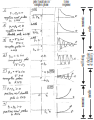
\includegraphics[width=6.5in]{../figures/2nd_order_poles.png}
	\caption{2nd order poles.}
\end{figure}



\begin{example}
Do example on stability of 2\textsuperscript{nd} order systems
\end{example}

%
%	\pagebreak
%	\renewcommand{\thepage}{}
%	\renewcommand\refname{References Cited}
%	\pagestyle{plain}
%	\bibliographystyle{Downey_NSF}
%	\bibliography{Chapter_1_Basic_Concepts}
%
%
%















\end{document}



% Chapter 3 Transfer Functions
\documentclass[12pt,letter]{article}
\usepackage{../downey_format}



\begin{document}
	
	% set the section number, along with figure and equation numbers
	\setcounter{section}{2}	
	\setcounter{figure}{0}    
	\renewcommand\thefigure{\thesection.\arabic{figure}}


	\section{Transfer Functions}

		Thus-far, this text has only considered forced vibrations for 1-DOF systems excited with forcing functions that can be easily expressed using either sin or cos examples. Therefore, the previously developed solutions are only acceptable for systems with known and simple excitations. This chapter will introduce the concept of transfer functions for solving vibration related problems. The transfer function, in particular the Laplace transfer function, is an important tool in the study of vibrations as it allows the practitioner to solve for the temporal response of a system for a variety of inputs using a single approach. Examples of force excitation that can be calculated include using this method include:
		\begin{itemize}
			\item sinusoidal
			\item base excitation
			\item impulse
			\item arbitrary input
			\item arbitrary periodic input
		\end{itemize}

			Consider the following system

			\begin{figure}[H]
				\centering
				\includegraphics[]{../figures/control_system.png}
				\caption{Generic system $H$ subjected to an input $F$ and its corresponding output $X$.}
				\label{fig:control_system}
			\end{figure}

			\noindent where $F$ is the input, $H$ is the system, and $X$ is the output from the system. This formulation is called the transfer-function approach and is commonly used for the formulation and solution of dynamic problems in the control literature. It can also be used for solving the various forced-vibration problems including those from complex or stochastic inputs. 

\subsection{Laplace Transforms}




\begin{review}
	\label{sec:Laplace_review}
				
		Laplace transforms, or more boradly integral transform, are a procedure for integrating the time ($t$) dependence of a function into a function of of position or space ($s$). By transforming the whole whole differential equation from the time domain into a lower order function of space the problem becomes easier to solve as the function can often be manipulated algebraically. 

		
		\begin{figure}[H]
			\centering
			\includegraphics[width=2.71in]{../figures/Pierre-Simon_de_Laplace.jpg}
			\caption{Portrait of Pierre-Simon Laplace by Johann Ernst Heinsius (1775).\protect\footnotemark[1] }
			\label{fig:Pierre-Simon_de_Laplace}
		\end{figure}
		
		\footnotetext[1]{Johann Ernst Heinsius, CC BY-SA 4.0 $<$https://creativecommons.org/licenses/by-sa/4.0$>$, via Wikimedia Commons}  

		The Laplace transform is named after mathematician and astronomer Pierre-Simon Laplace (23 March 1749 - 5 March 1827 ). Pierre-Simon Laplace was one of the greatest scientists of all time and is often considered the French Newton. He taught Napoleon at the \'Ecole Militaire in 1784, became a count of the empire in 1806, and a marquis in 1817 after the restoration of the monarchy. He is credited with advancements in engineering, mathematics, statistics, physics, astronomy, and philosophy; however, maybe his greatest achievement is not only surviving but benefiting from the change from the Ancien R\'egime $\rightarrow$ Bonaparte $\rightarrow$ Bourbon Restoration. 

	
		Of interest to this class is the Laplace transform ($\Laplace{\hspace{1ex}}$) of the function $f(t)$, expressed as $\Laplace{f(t)}$. Here, a Laplace transform is used as a method of solving the differential equations of motion by reducing the computation needed to that of integration and algebraic manipulation. 
		
		The definition of the Laplace transform of the function $f(t)$ is:
		
		\begin{equation}
				\Laplace{f(t)} = F(s) = \int_{0}^{\infty} f(t)e^{-st}dt
		\end{equation}
		where $s$ represents a variable in the complex plane (also called the $s$-plane) and $f(t)=0$ for all values of $t<0$. Here, the $s$ is a complex value. Lastly, the term $F(s)$ is a generic term that  represents the input to a system. As this class needs the derivatives of the base function, we will calculate these next:
		\begin{equation}
			\Laplace{\dot{f}(t)} = \int_{0}^{\infty} \dot{f}(t)e^{-st}dt = \int_{0}^{\infty} e^{-st}\frac{d[f(t)]}{dt}dt 
		\end{equation}		
		integration by parts yields:
		\begin{equation}
			\Laplace{\dot{f}(t)} = e^{-st}f(t)\Big|_0^\infty+s\int_{0}^{\infty}e^{-st}f(t)dt
		\end{equation}
		Astutely, it can be noticed that the second term $s\int_{0}^{\infty}e^{-st}f(t)dt$
		is the input to the system $F(s)$. Therefor, with a little rearranging this becomes:
		\begin{equation}
			\Laplace{\dot{f}(t)} = sF(s)-f(0)
		\end{equation}
		Taking the derivative of again yields:
		\begin{equation}
			\Laplace{\ddot{f}(t)} = s^2F(s)-sf(0)-\dot{f}(0)
		\end{equation}
		
		A few key points of the Laplace transforms are:
				
		\begin{itemize}
			\item The domain of the problem changes from the real number line ($t$) to the complex plane ($s$-plane).
			\item The integration of the Laplace transform changes differentiation into multiplication.
			\item The transform procedure is linear. Therefore, the transform of the linear combination of two transforms is the same as the linear transformation of these functions. 
			\item To move from the time domain to the complex number plane we typically use tables of pre-solved integral. 
			\item The function $x(t)$ can be obtained by taking the inverse Laplace transform defined as $x(t) = \Laplace{X(s)}^{-1}$
		\end{itemize}

			The Laplace transform can be calculated in symbolic form. In particular interest to this text is the Laplace form of the system input $F(s)$ and output $X(s)$. To expand the symbolic form of the Laplace transform for the system inputs are 
			and for system outputs:
			\begin{equation}
				\label{eq:laplace_f}
				\Laplace{f(t)} = F(s)
			\end{equation}		
			\begin{equation}
				\label{eq:laplace_f'}
				\Laplace{\dot{f}(t)} = sF(s)-f(0)
			\end{equation}	
			\begin{equation}
				\label{eq:laplace_f''}
				\Laplace{\ddot{f}(t)} = s^2F(s)-sf(0) - \dot{f}(0)
			\end{equation}	
			here, $f(0)$ and $\dot{f}(0)$ are the initial values of the function $f(t)$.  Furthermore, the for system outputs are:
			\begin{equation}
				\label{eq:laplace_x}
				\Laplace{x(t)} = X(s)
			\end{equation}		
			\begin{equation}
				\label{eq:laplace_x'}
				\Laplace{\dot{x}(t)} = sX(s)-x(0)
			\end{equation}	
			\begin{equation}
				\label{eq:laplace_x''}
				\Laplace{\ddot{x}(t)} = s^2X(s)-sx(0) - \dot{x}(0)
			\end{equation}	
			here, $x(0)$ and $\dot{x}(0)$ are the initial values of the function $x(t)$. 		
	
\end{review}


		\subsection{Transfer Function Method for Solving Vibrating Systems}
		
			As mentioned in the introduction to this chapter, a variety of systems can be solved for using the transfer function method. The procedure for using the Laplace transform to solve equations of motion expressed as an inhomogeneous ordinary differential equation is:
			\begin{enumerate}
				\item Take the Laplace transform of both sides of the EOM while treating the time derivatives symbolically.
				\item Solve for $X(s)$ in the obtained equation.
				\item Apply the inverse transform $x(t) = \Laplace{X(s)}^{-1}$
			\end{enumerate}
				
			\subsubsection{Free Vibration for Undamped Systems}
			Consider the undamped single-DOF system:
			\begin{figure}[H]
				\centering
				\includegraphics[]{../figures/1-DOF-spring_mass_horizontal.png}
				\caption{A spring mass model of a 1-DOF system.}
			\end{figure}
			\noindent The EOM for this system is a homogeneous differential equation becasue the right-hand side is equal to zero:
			\begin{equation}
				m\ddot{x}(t) + kx(t) = 0 
			\end{equation}
			Here we will leave the ``$(t)$'' for clarity to differentiate the time domain solution from Laplace solution ``$(s)$'' in the $s$-plane, as discussed in review~\ref{sec:Laplace_review}. The EOM can be rewritten in standard form as:
			\begin{equation}
				\ddot{x}(t) + \omega_n^2x(t) = 0 
			\end{equation}
			where the initial conditions at $t=0$ are $x(0)=x_0$ and $\dot{x}(0) = v_0$. Taking the Laplace transforms, in symbolic form using equations \ref{eq:laplace_x} - \ref{eq:laplace_x''}, of both sides of the EOM yields:
			\begin{equation}
				\big[s^2X(s) -sx_0 -v_0 \big] + \big[ \omega_n^2X(s) \big] =0
			\end{equation}
			using equations \ref{eq:laplace_x} and \ref{eq:laplace_x''} from section~\ref{sec:Laplace_review}. Solving for the output of the system $X(s)$ yields:
			\begin{equation}
			X(s) = \frac{sx_0 + v_0}{s^2 + \omega_n^2}
			\end{equation}
			We can expand this form of $X(s)$ to obtain equations listed in our Laplace Transform table:
			\begin{equation}
			X(s) = \frac{sx_0}{s^2 + \omega_n^2} + \frac{v_0}{s^2 + \omega_n^2}\cdot \frac{\omega_n}{\omega_n}
			\end{equation}
			This becomes:
			\begin{equation}
			X(s) = x_0\frac{s}{s^2 + \omega_n^2} + \bigg(\frac{v_0}{\omega_n}\bigg) \cdot \frac{\omega_n}{s^2 + \omega_n^2}
			\end{equation}
			
			Next, using the inverse Laplace transform $x(t) = \Laplace{X(s)}^{-1}]$ and the two following Laplace transforms (\#5 and \#6):
			\begin{equation}
			f(t) \text{ is cos}(\omega t) \text{ when }  F(s) \text{ is } \frac{s}{s^2+\omega^2} 
			\end{equation}
			\begin{equation}
			f(t) \text{ is sin}(\omega t)  \text{ when }  F(s) \text{ is } \frac{\omega}{s^2+\omega^2} 
			\end{equation}
			Therefore, we can obtain the solution for the system output $X(s)$ as:
			\begin{equation}
			x(t) = x_0 \text{cos}(\omega_n t) + \frac{v_0}{\omega_n}\text{sin}(\omega_n t)
			\end{equation}
			
			The same procedure can be used to calculate the under damped and forced responses. However, when calculating these responses the algebraic solution for $X(s)$, $s$ often contains quotients of polynomials. These Polynomial ratios may not be found in simple Laplace tables and must be solved using the method of partial fractions. An example of this procedure can be found in Appendix B of Inman. 

			\subsubsection{Forced Vibration (Impulse) for damped Systems}
		
			Shock loads on mechanical systems represent a very common source of vibration. These short-duration forces are also called called an impulse. An impulse excitation is defined as a force that is applied for a very short, or infinitesimal, length of time. An impulse is a nonperiodic force that is represented by the symbol $\delta$. The response of a system to an impulse load is the same as the system's free response provided that the correct initial conditions are applied. This is illustrated in the following where the applied force $F(t)$ is impulsive in nature (i.e., large magnitude over a very short time).
			
			\begin{figure}[H]
				\centering
				\includegraphics[width=0.5\textwidth]{../figures/unit_impulse.png}
				\caption{An impulse function with the impulse at $t=0$. }
			\end{figure}
			
			The impulse response function can be solved for analytically, however, we will solve it using the transfer function approach. Here we will consider the under-damped spring-mass system. First, assume that the system is at rest (no initial conditions). Next, we write the EOM as:
			\begin{equation}
			m\ddot{x} +c\dot{x} +kx = \delta(t)
			\end{equation}
			Taking the Laplace transform of both sides of the equation yields 
			\begin{equation}
			m\big(s^2X(s)-sx(0) - \dot{x}(0)\big) + c\big(sX(s)-x(0)\big) +kX(s) =1
			\end{equation}
			note that the $\Laplace{\delta}=1$ per \#1 in the transform table. However, if we assume zero initial conditions (a system at rest when the impulse happens), the equation simplifies to. 
			\begin{equation}
			ms^2X(s) + csX(s) +kX(s) =1
			\end{equation}
			or
			\begin{equation}
			(ms^2 + cs +k)X(s) =1
			\end{equation}
			Solving this equation for $X(s)$:
			\begin{equation}
			X(s) = \frac{1}{m} \cdot \frac{1}{s^2 + 2 \zeta \omega_n s + \omega_n^2}
			\end{equation}
			Again, the mass is extracted to develop a formulation that can be found in the Laplace tables. Setting the constraint that $\zeta<1$ and consulting \#10 in the table for Laplace transforms results in:
			\begin{equation}
			x(t) = \frac{1}{m \omega_d} e^{-\zeta \omega_n t} \text{sin}(\omega_dt)
			\end{equation}
			where this is the general solution for a damped system subjected to an impulse loading function. For the undamped case a solution can be obtained by setting $\zeta=0$. This Results in the following form for the undamped case:
			\begin{equation}
			x(t) = \frac{1}{m \omega_n}\text{sin}(\omega_n t)
			\end{equation}
			Below is a typical response for both a undamped and underdamped 1-DOF system subject to an impulse response at $t=0$ seconds. 
			\begin{figure}[H]
				\centering
				\includegraphics[]{../figures/response_impulse.png}
				\caption{Temporal responses from a underdamped and undamped 1-DOF systems to a impulse response function.}
			\end{figure}


\subsubsection{Arbitrary Inputs to a System}
\label{sec:impulse_inputs}
The time domain response of a system to an arbitrary input force in time can be calculated using a series of impulses as shown in figure \ref{fig:Arbitary_excitation_forces}. This method allows the practitioner to easily calculate the response of an arbitrary input to a system using a single expression executed in a ``for loop''. This type of analysis is often more efficient in terms of programming than more direct methods such as the transfer functions sown in this text. 

\begin{figure}[H]
	\centering
	\includegraphics[]{../figures/Arbitary_excitation_forces.png}
	\caption{Generalized response showing that any signal can be represented as a series of impulse signals. }
	\label{fig:Arbitary_excitation_forces}
\end{figure}



\begin{example}


In testing, an hammer is used to excite a 1-DOF system with an impact (i.e. impulse), however, the hammer ascendantly impacts the system twice. The first impact has a force of 0.2 N, while the second has a force of 0.1 N and happens 0.1 seconds after the first impact. Plot the response for the double impact. The system has the parameters $m$ = 1 kg, $c$ = 0.5 kg/s, k = 4 N/m. 

\noindent\textbf{Solution:} First, we can define the forcing function as:

\begin{equation}
	F(t) = 0.2 \delta (t) + 0.1 \delta(t-\tau)
\end{equation}
where $\tau$ is the offset between the first and second impacts. Next, considering that the unit impulse has a magnitude of 1 we can obtain solutions for the first impact by first writing it's EOM:

\begin{equation}
m\ddot{x}(t) +c\dot{x}(t) +kx(t) =0.2 \delta(t)
\end{equation}
Taking the Laplace transform of both sides of the equation yields 
\begin{equation}
m\big(s^2X(s)-sx(0) - \dot{x}(0)\big) + c\big(sX(s)-x(0)\big) +kX(s) = 0.2
\end{equation}
However, assuming zero initial conditions, the equation simplifies to. 
\begin{equation}
(ms^2 + cs +k)X(s) = 0.2
\end{equation}
Solving this equation for $X(s)$:
\begin{equation}
X(s) = \frac{0.2}{m} \cdot \frac{1}{s^2 + 2 \zeta \omega_n s + \omega_n^2}
\end{equation}
Again, consulting \#10 in the table for Laplace transforms results in:
\begin{equation}
x_1(t) = \frac{0.2}{m \omega_d} e^{-\zeta \omega_n t} \text{sin}(\omega_dt)
\end{equation}
where this is the general solution for a damped system subjected to an impulse loading function. The second impact can now be solved for using the same method. However, now the time $(t)$ must be offset by $(\tau)$ to allow the impact to still be located at $t=0$ in terms of the second impact. This results in:
\begin{equation}
	x_1(t) = \frac{0.2}{m \omega_d} e^{-\zeta \omega_n t} \text{sin}(\omega_dt)
\end{equation}
\begin{equation}
	x_2(t) = \frac{0.1}{m \omega_d} e^{-\zeta \omega_n (t-\tau)} \text{sin}\big(\omega_d(t-\tau)\big)
\end{equation}
Next, using the knowledge that the systems are linear and that the Laplace transform of a linear combination of two transforms is the same as the linear transformation of these functions we can build the piecewise function:

\[
  x(t) = 
  \begin{cases}
\frac{0.2}{m \omega_d} e^{-\zeta \omega_n t} \text{sin}(\omega_dt) & \text{if } t < \tau \\
\frac{0.2}{m \omega_d} e^{-\zeta \omega_n t} \text{sin}(\omega_dt)  + \frac{0.1}{m \omega_d} e^{-\zeta \omega_n (t-\tau)} \text{sin}\big(\omega_d(t-\tau)\big) & \text{if } \tau \leq t 
  \end{cases}
\]


For the mass, damping, and stiffness values given above this can be plotted as:
\begin{figure}[H]
	\centering
	\includegraphics[width=0.75\textwidth]{../figures/response_double_impact.png}
\end{figure}

\end{example}




		\subsection{Laplace method in Controls}

		Again, consider the Laplace system:
		\begin{equation}
				\Laplace{f(t)} = F(s) = \int_{0}^{\infty} f(t)e^{-st}dt
		\end{equation}
		where:
		\begin{equation}
			\int_{0}^{\infty} = \lim_{p \rightarrow \infty} \int_{0}^{p}
		\end{equation}
		exists. For now, $s \in \mathbb{R}$ (real). Later, we will let $s \in \mathbb{C} $ (complex). For any given $F(s)$, we can find the original $F(t)$ using the pairing method. 
		\begin{equation}
			f(t) \overset{LT}{\underset{ILT}\rightleftarrows} F(s) 
		\end{equation}
		this can also be written as:
		\begin{equation}
		\text{LT pair} =
			\begin{cases}
			F(s) & \Laplace{f(t)} \\
			f(t) & \Laplace{F(s)}^{-1} \\
			\end{cases}
		\end{equation}

		\subsubsection{Laplace transform of exponential function}

		Consider the exponential function,
		\begin{equation}
		\Laplace{e^{p_0t}} = \frac{1}{s -p_0} 
		\end{equation}
		where
		$f(t) = e^{p_0t}$ and $F(s) = \frac{1}{s -p_0} $. As $F(s) \rightarrow \infty $, $s \rightarrow p_0$, therefore $p_0$ is a pole of the system. This is shown in Fig.~\ref{fig:S_space_exp_pt}.	

		\begin{equation}
		\text{LT pair} =
			\begin{cases}
			f(t) & e^{p_0t} \\
			F(s) & \frac{1}{s -p_0} \\
			\end{cases}
		\end{equation}

	
		\begin{figure}[H]
			\centering
			\includegraphics[width=6.5in]{../figures/T_and_S_space_exponential_function.png}
			\caption{Function $e^{p_0t}$ with $p_0=5$; showing the (a) time domain and; (c) the s-space.}
			\label{fig:S_space_exp_pt}
		\end{figure}



\begin{mdframed}[middlelinewidth=0.5mm]
\begin{center}
\gr{Proof}
\end{center}
Show that
\begin{equation}
\Laplace{e^{p_0t}} = \frac{1}{s -p_0} 
\end{equation}
Again, consider the Laplace system:
\begin{equation}
		\Laplace{f(t)} = F(s) = \int_{0}^{\infty} f(t)e^{-st}dt
\end{equation}
therefore, 
\begin{equation}
	\int_{0}^{\infty}f(t)e^{-s t} dt =  \int_{0}^{\infty}e^{p_0t}e^{-st}dt = \int_{0}^{\infty}e^{-(s-p_0)t}dt
\end{equation}
Change of variables can be used such that:
\begin{align}
(s-p_0)t &= t^*  \\ \nonumber
(s-p_0)dt &= dt^*  \\ \nonumber
dt &= \frac{1}{s-p_0}dt^*
\end{align}
therefore
\begin{align}
	\int_{0}^{\infty}e^{-(s-p_0)} dt &=  \int_{0}^{\infty}e^{-t^*}\frac{1}{s-p_0}dt^*  \\ \nonumber
	&= \frac{1}{s-p_0} \int_{0}^{\infty}e^{-t^*} dt^*  \\ \nonumber
&= \frac{1}{s-p_0} \big(-e^{-t^*}\big) \bigg|^\infty_0 \\ \nonumber
&= \frac{-1}{s-p_0} \big(e^{-t^*}\big) \bigg|^\infty_0 \\ \nonumber
&= \frac{-1}{s-p_0} \big[e^{-\infty - e^0}\big] \\ \nonumber
&= \frac{-1}{s-p_0} (-1) \\ \nonumber
&= \frac{1}{s-p_0}
\end{align}
Therefore, it can be shown that:
\begin{equation}
\Laplace{e^{p_0t}} = \frac{1}{s -p_0} 
\end{equation}
\end{mdframed}



		\subsubsection{Laplace transform of step function}

		\begin{equation}
		\text{LT pair} =
			\begin{cases}
			f(t) & 1(t) , \; \; \; t>0 \\
			F(s) & \frac{1}{s} \\
			\end{cases}
		\end{equation}


		\begin{figure}[H]
			\centering
			\includegraphics[width=6.5in]{../figures/T_and_S_space_step_function}
			\caption{Step function; showing the (a) time domain and; (c) the s-space.}
			\label{fig:T_and_S_space_step_function}
		\end{figure}


\begin{mdframed}[middlelinewidth=0.5mm]
\begin{center}
\gr{Proof}
\end{center}
Show that
\begin{equation}
\Laplace{1(t)} = \frac{1}{s}
\end{equation}
This can be done as:
\begin{align}
	\Laplace{1(t)} &=  \int_{0}^{\infty}1 \cdot e^{-st} dt \\ \nonumber
	&= \int_{0}^{\infty}e^{-st} dt  \\ \nonumber
&= \frac{-1}{s}e^{-st}\bigg|^\infty_0 \\ \nonumber
&= \frac{1}{s} 
\end{align}
\end{mdframed}

		\subsubsection{Laplace transform of ramp function}

		\begin{equation}
		\text{LT pair} =
			\begin{cases}
			f(t) & t, \; \; \; t>0 \\
			F(s) & \frac{1}{s^2} \\
			\end{cases}
		\end{equation}

		\begin{figure}[H]
			\centering
			\includegraphics[width=6.5in]{../figures/T_and_S_space_ramp_function}
			\caption{Ramp function; showing the (a) time domain and; (c) the s-space.}
			\label{fig:T_and_S_space_ramp_function}
		\end{figure}





\begin{mdframed}[middlelinewidth=0.5mm]
\begin{center}
\gr{Proof}
\end{center}
Show that
\begin{equation}
\Laplace{t} = \frac{1}{s^2}
\end{equation}
This can be done as:
\begin{equation}
\Laplace{t} =  \int_{0}^{\infty}t \cdot e^{-st} dt
\end{equation}
integration by parts leads to:
\begin{equation}
d[uv] = udv + vdu \rightarrow vdu = d[uv] - udv
\end{equation}
where
\begin{equation}
 \int_{a}^{b} vdu = uc \bigg|_a^b - \int_{a}^{b} u dv
\end{equation}
which leads to:
\begin{equation}
du = e^{-st};  \; \; \; u = \frac{1}{-s}e^{-st}
\end{equation}
or more simply, 
\begin{equation}
du = 1;  \; \; \; u = t
\end{equation}
Using these expressions, we get
\begin{align}
	 \int_{0}^{\infty}t \cdot e^{-st} dt &=  \frac{t}{-s} e^{-s t} \bigg|_0^\infty - \int_{0}^{\infty}\frac{-1}{-s}e^{-st} dt \\ \nonumber
	&= \frac{1}{s} \int_{0}^{\infty} e^{-st} dt \\ \nonumber
&= \bigg[\frac{1}{s}\bigg]\bigg[\frac{1}{s}\bigg],\text{ as }  \Laplace{1(t)} =  \int_{0}^{\infty} e^{-st} dt  = \frac{1}{s} \\ \nonumber
&= \frac{1}{s^2}
\end{align}
\end{mdframed}


		\subsubsection{Laplace transform shifted step function}

		\begin{equation}
		\text{LT pair} =
			\begin{cases}
			f(t) & 1(t-\tau) \\
			F(s) & e^{-\tau s} \frac{1}{s} \\
			\end{cases}
		\end{equation}

		\begin{figure}[H]
			\centering
			\includegraphics[width=6.5in]{../figures/T_and_S_shifted_space_step_function}
			\caption{Shifted step function; showing the (a) time domain and; (c) the s-space. }
			\label{fig:Laplace_shifted_step_transform}
		\end{figure}

\begin{mdframed}[middlelinewidth=0.5mm]
\begin{center}
\gr{Proof}
\end{center}
Show that
\begin{equation}
\Laplace{1\cdot(t-\tau)} =e^{-\tau s} \frac{1}{s}
\end{equation}
This can be done as:
\begin{equation}
\end{equation}
\begin{align}
	 \Laplace{1\cdot(t-\tau)}  &=  \int_{0}^{\infty} 1 (t-\tau) e^{-st} dt \\ \nonumber
	&=  \int_{0}^{\tau} 0 \cdot  e^{-st} dt + \int_{\tau}^{\infty} e^{-st} dt  \\ \nonumber
	&=  \int_{\tau}^{\infty} e^{-st} dt  \\ \nonumber
\end{align}
using a change of variable substitution, 
\begin{equation}
t^* = t-\tau; \; \; \; t = t^* + \tau; \; \; \; dt^* = dt
\end{equation}
Therefore
\begin{align}
	 \int_{\tau}^{\infty} e^{-st} dt  &=  \int_{0}^{\infty}e ^ {-s (t^* + \tau)} dt^* \\ \nonumber
	&=  e^{-s \tau}  \int_{0}^{\infty}e ^ {-s (t + \tau^*)} dt^*   \\ \nonumber
	&=  e^{-s \tau} \frac{1}{s}  \\ \nonumber
\end{align}
connecting the start of proof to the end shows:
\begin{equation}
\Laplace{1\cdot(t-\tau)} =e^{-\tau s} \frac{1}{s}
\end{equation}
\end{mdframed}


		\subsubsection{Laplace transform pulse function}

		\begin{equation}
		\text{LT pair} =
			\begin{cases}
			f(t) & p(t; \; \; \tau) \\
			F(s) & \frac{1-e^{-s \tau}}{s \tau}
			\end{cases}
		\end{equation}

		\begin{figure}[H]
			\centering
			\includegraphics[width=6.5in]{../figures/T_and_S_pulse_function}
			\caption{Pulse function; showing the (a) time domain and; (c) the s-space.}
			\label{fig:Laplace_pulse_transform}
		\end{figure}


\begin{mdframed}[middlelinewidth=0.5mm]
\begin{center}
\gr{Proof}
\end{center}
Show that
\begin{equation}
\Laplace{p(t;\tau)} = \frac{1-e^{-st\tau}}{s \tau}
\end{equation}
This can be done by writing the pulse as a step up followed by a step down at $t=\tau$ and scaled to be $\frac{1}{\tau}$, i.e.,:
\begin{equation}
p(t;\tau) = \frac{1}{\tau}1(t) - \frac{1}{\tau} 1 (t-\tau)
\end{equation}
given that
\begin{equation}
\Laplace{1(t)} =  \frac{1}{s}, \; \; \; \Laplace{1 (t-\tau)} = e^{-s \tau} \frac{1}{s}
\end{equation}
the $s$ domain of $p(t;\tau)$ is expressed as
\begin{equation}
F(s) =   \frac{1}{\tau}  \frac{1}{s}  - \frac{1}{\tau} e^{-s \tau} \frac{1}{s}
\end{equation}

\begin{align}
	 F(s) &=   \frac{1}{\tau}  \frac{1}{s}  - \frac{1}{\tau} e^{-s \tau} \frac{1}{s} \\ \nonumber
	&=  \frac{1-e^{-s \tau}}{s \tau} \\ \nonumber
\end{align}
connecting the start of proof to the end shows:
\begin{equation}
\Laplace{p(t;\tau)} = \frac{1-e^{-s \tau}}{s \tau}
\end{equation}

\end{mdframed}



		\subsubsection{Laplace transform impulse function}

		\begin{equation}
		\text{LT pair} =
			\begin{cases}
			f(t) & \delta(t) \\
			F(s) & 1 \\
			\end{cases}
		\end{equation}

		\begin{figure}[H]
			\centering
			\includegraphics[width=6.5in]{../figures/T_and_S_impulse_function}
			\caption{Impulse function; showing the (a) time domain and; (c) the s-space.}
			\label{fig:T_and_S_impulse_function}
		\end{figure}


\begin{mdframed}[middlelinewidth=0.5mm]
\begin{center}
\gr{Proof}
\end{center}
Show that
\begin{equation}
\Laplace{\delta(t)} = 1
\end{equation}
Consider $\delta(t)$ as the limit of $p(t;\tau) $ as $\tau \rightarrow 0$ and take the Laplace Transform. 
\begin{equation}
\delta(t) = \lim\limits_{\tau \rightarrow 0} p(t;\tau) 
\end{equation}
taking the Laplace transform
\begin{align}
\Laplace{\delta(t)} &= \lim\limits_{\tau \rightarrow 0} \Laplace{p(t;\tau)} \\ \nonumber
&=  \lim\limits_{\tau \rightarrow 0} \frac{1-e^{-st}}{s \tau}
\end{align}
taking the limit of this in ${1-1}/0 = 0/0$. Applying L'Hospital's (loh-pee-TAHL) rule, 
\begin{align}
\lim\limits_{\tau \rightarrow 0} \frac{ \frac{\partial}{\partial \tau} \big(     1-e^{-s t}    \big)  }{ \frac{\partial}{\partial \tau} (s \tau)} &= \lim\limits_{\tau \rightarrow 0} \frac{- \big(-s e^{-s \tau \big)}}{s}  \\ \nonumber
&=  \lim\limits_{\tau \rightarrow 0} e^{-s \tau} \\ \nonumber
&= 1
\end{align}
connecting the start of proof to the end shows:
\begin{equation}
\Laplace{\delta(t)} = 1
\end{equation}

Moreover, this can also be done useint the localization property of the delta function. Recall that
\begin{equation}
\int_{0}^{\infty} \delta(t) g(t) dt = g(0)
\end{equation}
then
\begin{align}
\Laplace{\delta(t)} &= \int_{0}^{\infty} \delta(t) e^{-s t} dt; \text{ where } g(t) = e^{-s t} \\ \nonumber
&= e^{-s t}\big|_{t=0} \\ \nonumber
&= e^0 \\ \nonumber
&= 1
\end{align}
Again, connecting the start of proof to the end shows:
\begin{equation}
\Laplace{\delta(t)} = 1
\end{equation}
\end{mdframed}

\subsection{Properties of Laplace Transforms}


There are a variety of Laplace transforms that can assist in moving between $f(t)$ and $F(s)$. Importantly, the differentiation, integration, time shift, and final value theorems are useful as they allow you to expand a Laplace table by taking the Laplace transform of functions without using the Laplace transform definition. Moreover, these properties are used extensively during control system design so being fluent in them makes you a better designer. A subset of these are shown in Table~\ref{table:laplace_theorems} while some of the more important ones are derived in the following sub sections. 

The goal of studying the Laplace transform properties is to be able to Laplace Transform a differential equation with initial conditions and to relate differentiation and integration in the time domain to their counterparts in the s-domain domain. 

\begin{table}[H]
\centering
\caption{A list of important Laplace Transform theorems used in control.}
\label{table:laplace_theorems}
\begin{tabular}{@{}lll@{}}
\toprule
number & theorem & name \\ \midrule
1 & $ 	\Laplace{f(t)} = F(s) = \int_{0}^{\infty} f(t)e^{-st}dt$ & definition \\
2 & $ 	\Laplace{kf(t)} = kF(s) $ & linearity theorem \\
3 & $ \Laplace{f_1(t)+f_2(t)} = F_1(s) + F_2(s) $ & linearity theorem \\
4 & $ \Laplace{e^{-at}f(t)} = F(s+a)$ & frequency shift theorem \\
5 & $ \Laplace{f(t-t_0)} = e^{-t_0s}F(s) $ & time shift theorem \\
6 & $ \Laplace{e^{s_0t}f(t)} = F(s-s_0)$ & time shift theorem \\
7 & $ \Laplace{f(at)} = \frac{1}{a}F \frac{s}{a} $ & scaling theorem \\
8 & $\Laplace{f'(t)} = sF(s) \text{, if } f(0) = 0   $ & differentiation theorem \\
9 & $ \Laplace{f''(t)} = s^2F(s) \text{, if } f'(0) = f(0) = 0  $ & differentiation theorem \\
10 & $ \Laplace{f^{n}(t)} = s^{n}F(s) \text{, if } f^{n-1}(0) = \cdots = f'(0) = f(0) = 0 $ & differentiation theorem \\
11 & $ \Laplace{\int_{0}^{t}f(t^*)dt^*} = \frac{1}{s}F(s) $ & integration theorem\\
12 & $ f(\infty)  = \lim\limits_{s\rightarrow 0} [s F(s)] $ & final value theorem$^1$ \\
13 & $ f(0+)  = \lim\limits_{s\rightarrow \infty} [s F(s)] $ & initial value theorem$^2$ \\ \bottomrule
\end{tabular}
\end{table}
\vspace{-2ex}
\noindent {\small $^1$This requires all roots of the denominator of $F(s)$ to have negative real parts, and no more than one can be on the origin of the real axis.} \\
\noindent {\small$^2$This requires that $f(t)$ be continuous or have a step discontinuity at $t=0$. This does not allow for impulses at $t=0$.}




\subsubsection{Differentiation Property}

The Laplace transforms can be simplified if we assume $ f(0) = 0$, where these are the terms associated with the initial conditions. This is shown as:
\begin{align}
\Laplace{f'(t)} &= sF(s) \text{, if } f(0) = 0   \\
\Laplace{f''(t)} &= s^2F(s) \text{, if } f'(0) = f(0) = 0  \nonumber \\
&\vdots  \nonumber \\
\Laplace{f^{(n)}(t)} &= s^{(n)}F(s) \text{, if } f^{(n-1)}(0) = \cdots = f'(0) = f(0) = 0 \nonumber  
\end{align}
Recall that differentiation in the time domain becomes multiplication by s in the s-domain.


\begin{mdframed}[middlelinewidth=0.5mm]
\begin{center}
\gr{Proof}
\end{center}

\noindent \textbf{Method 1:}
Show that $\Laplace{f'(t)} = s F(s)$ if $f(0) = 0$;
\begin{equation}
\Laplace{f'(t)} = \int_{0}^{\infty} f'(t)e^{-st}dt 
\end{equation}
integration by parts $udv = d(uv) -vdu$ where
\begin{align}
e^{-st} &= u   \\
f'(t)dt &= dv  \nonumber \\
f(t) &= v  \nonumber \\
-se^{-st} &= du   \nonumber
\end{align}
leads to
\begin{equation}
\Laplace{f'(t)} = f(t)e^{-st}\big|_{0}^{\infty} - \int_{0}^{\infty}f(t)(-se^{-st})dt
\end{equation}
further simplification results in:
\begin{align}
\Laplace{f'(t)} &= f(\infty)e^{- \infty} - f(0) + s \int_{0}^{\infty} f e^{-s t} dt   \\
 &= s F(s) -f(0)  \nonumber \\
 &= s F(s)  \nonumber
\end{align}
where $F(s) = \int_{0}^{\infty} f e^{-s t} dt$, $e^{- \infty}=0$, and $f(0) = 0$. Therefore, 
\begin{equation}
\Laplace{f'(t)} = s F(s)
\end{equation}

\noindent \textbf{Method 2:}
Show that $\Laplace{f'(t)} = s F(s)$ if $f(0) = 0$. Denote $f(t) = f'(t)$, therefore:
\begin{align}
G(s) &= \Laplace{g(t)} = \Laplace{f'(t)} = sF(s)  \\
\Laplace{f''(t)} &= \Laplace{g'(t)} = s\Laplace{G(s)} = s^2F(s)  \nonumber
\end{align}
by induction it can be shown that 
\begin{equation}
\Laplace{f'(t)} = s F(s)
\end{equation}

Bottom line: ``to differentiate, multiply by $s$'', provided $f(0) =0$, $f'(0) =0$, etc. Else, need to subtract them $\Laplace{f'(t)} = sF(s) -f(0)$ etc. 
\end{mdframed}

\subsubsection{Integration Property}

The integral of $f(t)$ is
\begin{equation}
\Laplace{\int_{0}^{t}f(t^*)dt^*} = \frac{1}{s}F(s)
\end{equation}
where $t^*$ is the dummy variable to integrate over as $t$ is used for the limit.  The main take away here is that integration in the time domain becomes division by s in the s-domain.

\begin{mdframed}[middlelinewidth=0.5mm]
\begin{center}
\gr{Proof}
\end{center}

\noindent Show that $\Laplace{\int_{0}^{t}f(t^*)dt^*} = \frac{1}{s}F(s)$. Denote $g(t) =  \int_{0}^{t}f(t^*)dt^*$, then:
\begin{equation}
g'(t) = f(t)\text{; } g(0) = 0
\label{eq:laplace_integration_property}
\end{equation}
taking the Laplace of the left hand side of this expression yields:
\begin{equation}
\Laplace{g'(t)} = s\Laplace{g(t)} = s \Laplace{\int_{0}^{t}f(t^*)dt^*}
\end{equation}
the Laplace of the right hand side of this expression yields:
\begin{equation}
\Laplace{f(t)} = F(s)
\end{equation}
therefore, by equation~\ref{eq:laplace_integration_property} 
\begin{equation}
s \Laplace{\int_{0}^{t}f(t^*)dt^*} = F(s)
\end{equation}
divide by $s$ to get 
\begin{equation}
\Laplace{\int_{0}^{t}f(t^*)dt^*} = \frac{1}{s}F(s)
\end{equation}

Bottom line: ``to integrate, divide by $s$''. 
\end{mdframed}


\subsubsection{Time Shift Property}
%\todo{should this be called $\tau$ and not $t_0$?}
To shift in $t$
\begin{equation}
\Laplace{f(t-t_0)} = e^{-t_0s}F(s)
\end{equation}
To shift in $s$
\begin{equation}
\Laplace{e^{s_0t}f(t)} = F(s-s_0)
\end{equation}
A shift in the $t$ domain
		\begin{figure}[H]
			\centering
			\includegraphics[width=3.5in]{../figures/shift_properties}
			\caption{Shift of a signal in the $t$ domain.}
			\label{fig:shift_properties}
		\end{figure}
Note that:
\begin{itemize}[noitemsep, topsep=0pt]
\item Function $f(t)$ is zero for $t<0$ arrangement
\item Function $f(t-t_0)$ is zero for $t<t_0$ arrangement
\end{itemize}


\begin{mdframed}[middlelinewidth=0.5mm]
\begin{center}
\gr{Proof}
\end{center}
\noindent \textbf{t-domain}

For a shift in $t$, show that $\Laplace{f(t-t_0)} = e^{-t_0s}F(s)$
\begin{align}
\Laplace{f(t-t_0)} &= \int_0^\infty f(t-t_0) e^{-st}dt  \\
&= \int_0^{t_0} 0 \cdot e^{-st}dt + \int_{t_0}^\infty f(t-t_0) e^{-st}dt  \nonumber \\
&= \int_{t_0}^\infty f(t-t_0) e^{-st}dt  \nonumber
\end{align}
using a change of variables:
\begin{align}
t* &= t-t_0 \rightarrow t = t*+t_0\\
dt* &= dt  \nonumber
\end{align}
therefore, 
\begin{align}
\Laplace{f(t-t_0)} &= f(t^*)e^{-s(t^*+t_0)}dt^*     \\
&= e^{-s t_0} \int_0^{\infty} f(t^*)e^{-s t^*}dt^*  \nonumber \\
&= e^{-s t_0} F(s)  \nonumber
\end{align}
lastly, we can show that:
\begin{equation}
\Laplace{f(t-t_0)} = e^{-t_0s}F(s)
\end{equation}

\noindent \textbf{s-domain}

For a shift in $s$, show that $\Laplace{e^{s_0t}f(t)} = F(s-s_0)$
\begin{align}
\Laplace{e^{s_0t}f(t)} &= \int_0^{\infty} e^{-s_0 t}  f(t)e^{-s t}dt  \nonumber \\
&=\int_0^{\infty} f(t)e^{-(s-s_0) t}dt  \nonumber \\
&= F(s-s_0)
\end{align}

\end{mdframed}

 


\subsubsection{Final Value Theorem}
This applies to the steady state response $x(\infty)$ which can also be denoted with a subscript ss as $x_{ss}$ where

\begin{equation}
x_{ss} = x(\infty)  = \lim\limits_{t\rightarrow \infty} [x(t)]  =  \lim\limits_{s\rightarrow 0} [s X(s)]
\end{equation}
therefore, 
\begin{equation}
x_{ss} =  \lim\limits_{s\rightarrow 0} [s X(s)]
\end{equation}


\begin{mdframed}[middlelinewidth=0.5mm]
\begin{center}
\gr{Proof}
\end{center}

Prove that $x_{ss} = \lim\limits_{s\rightarrow 0} s X(s)$. Starting with, 
\begin{equation}
\Laplace{\dot{x}(t)} = s X(s)\text{, } x(0)=0
\end{equation}
by definition
\begin{equation}
\Laplace{\dot{x}(t)} = \int_0^{\infty} \dot{x}(t)e^{-s t}dt
\end{equation}
combing the last two equations yields
\begin{equation}
\int_0^{\infty} \dot{x}(t)e^{-s t}dt = s X(s)
\end{equation}
taking the limit as $s \rightarrow 0$ results in 
\begin{equation}
\lim\limits_{s \rightarrow 0} \bigg[ \int_0^{\infty} \dot{x}(t)e^{-s t}dt \bigg] = \lim\limits_{s \rightarrow 0}[s X(s)]
\label{eq:final_value_theorem_eq_1}
\end{equation}
but
\begin{equation}
\lim\limits_{s \rightarrow 0} [ e^{-s t}] = e^0 = 1
\end{equation}
therefore, the left hand side of equation~\ref{eq:final_value_theorem_eq_1} simplifies to 
\begin{equation}
\int_0^{\infty} \dot{x}(t)dt = x(t)  \big|_{0}^{\infty} = x(\infty) = x_{ss}
\end{equation}
inserting this term back into equation~\ref{eq:final_value_theorem_eq_1} yields the desired proof
\begin{equation}
x_{ss} =  \lim\limits_{s\rightarrow 0} [s X(s)]
\end{equation}

\end{mdframed}


\subsection{Convolutional property of Laplace Transforms}



\begin{align}
\label{eq:convolutional_property_of_laplace_transforms}
\Laplace{G(s) \cdot F(s)}^{-1} &= \Laplace{F(s) \cdot G(s)}^{-1} \\
&= \int_0^t f(\tau) g(t-\tau) d \tau \nonumber \\
&= (f * g)(t)  \nonumber \\ 
&= x(t) \nonumber
\end{align}
where $f(\tau)$ is the excitation function and $g(t-\tau)$ is the impulse response of the function. Convolution expresses the system response $x(t)$ to a complicated excitation $f(\tau)$ as an integral using the impulse response $g(t)$  shifted by $\tau$ to $t-\tau$. 
The integral in equation~\ref{eq:convolutional_property_of_laplace_transforms} is not easily computed in the time domain, however, Laplace transforms make it easy using a three step process:
\begin{enumerate}[noitemsep,topsep=0pt]
\item Calculate $F(s) = \Laplace{f(t)} $, $G(s) = \Laplace{g(t)}$
\item Multiply $F(s)G(s)$
\item Take the inverse Laplace transform to get $x(t)$
\end{enumerate} 

\subsection{Transfer Function for Response to Random Inputs}

			Consider the following system
			\begin{figure}[H]
				\centering
				\includegraphics[]{../figures/transfer_function_system.png}
				\caption{Generic block diagram of a system $H(s)$ subjected to an input $F(s)$ and its corresponding output $X(s)$ where the $(s)$ denotes that the considered system is in the $s$-plane.}
				\label{fig:transfer_function_system}
			\end{figure}
			\noindent where $F(s)$ is the input, $H(s)$ is the system, and $X(s)$ is the output from the system. This formulation is called the transfer-function approach and is commonly used for the formulation and solution of dynamic problems in the control literature. It can also be used for solving the various forced-vibration problems including those from complex or stochastic inputs. 
	
\subsubsection{Defining the transfer function $\mathbf{H(s)}$}

Again, consider the generic system represented in figure~\ref{fig:transfer_function_system}. For this system representation, $F(s)$ is the Laplace of the transform of the driving force and $H(s)$ is the Laplace transform of the response of the system $h(t)$. 

We need to define transfer function $H(s)$ for a generic system. To do this let us show the reasoning behind the transfer function. Here we will show that the output of any system ($x(t)$) can be related to the input of the system ($f(t)$) through a series of polynomial coefficients ($a$ and $b$). Consider the general $n^{th}$-order linear, time-invariant differential equation that governs the behavior of the dynamic system.

\begin{equation}
a_n\frac{d^nx(t)}{dt^n} + a_{n-1}\frac{d^{n-1}x(t)}{dt^{n-1}} + ... + a_0x(t) = b_m\frac{d^mf(t)}{dt^m} + b_{m-1}\frac{d^{m-1}f(t)}{dt^{m-1}} + ... + b_0f(t)
\end{equation} 
where $x(t)$ is the output and $f(t)$ is the input. Note that this is similar to the formulation we have had before for the EOM. Taking the Laplace transformation of both side of the above equation yields

\begin{eqnarray}
&a_ns^nX(s) + a_{n-1}s^{n-1}X(s) + ... + a_0X(s) + \text{initial condition for } x(t) =   \\
&b_ms^mF(s) + b_{m-1}s^{m-1}F(s) + ... + b_0F(s) + \text{initial condition for } f(t)  \nonumber
\label{eq:transfer_function_polynominal_expansion}
\end{eqnarray}
It can be seen that this equation is a purely algebraic expression. If we assume the initial conditions to be zero, the equation reduces to the following:
\begin{eqnarray}
(a_ns^n + a_{n-1}s^{n-1} + ... + a_0)X(s) =  (b_ms^m + b_{m-1}s^{m-1} + ... + b_0)F(s) 
\label{eq:transfer_algebraic_expression}
\end{eqnarray}
if we rearrange equation \ref{eq:transfer_algebraic_expression} to solve for the relationship between the Laplace variables $\big( X(s)$ and $F(s) \big)$ and the algebraic expressions we get:
\begin{equation}
\frac{X(s)}{F(s)} = \frac{b_ms^m + b_{m-1}s^{m-1} + ... + b_0}{a_ns^n + a_{n-1}s^{n-1} + ... + a_0}
\end{equation}
this shows that the ratio of the input algebraic expressions over the output algebraic expressions is equal to the ratio of the output Laplace variable over the input Laplace variable. This shows that we can relate the Laplace variables to the algebraic expressions. Therefore, we can define the transfer function $H(s)$ as: 
\begin{equation}
G(s) = H(s) = \frac{X(s)}{F(s)}
\label{eq:transfer_function}
\end{equation}

In a more formal term, the transfer function that is defined as: ``The ratio of the Laplace transforms of the output or response function to the Laplace transform of the input or forcing function assuming zero initial conditions''. Note that many texts define $H(s)$ as $G(s)$ and this is simply a matter of syntax. 

Equation \ref{eq:transfer_function} can be rearranged to show that the output of the system $X(s)$, can be obtained if we know the input $F(s)$ and the transfer function $H(s)$:
\begin{equation}
 X(s) = H(s)F(s)
\end{equation}	


\subsubsection{Transfer Function method (Steady-State solution)}

Considering the forced system:
\begin{figure}[H]
	\centering
	\includegraphics[width=0.4\textwidth]{../figures/1-DOF-spring_dashpot_mass_horizontal_forced.png}
	\caption{A spring-dashpot-mass model of a 1-DOF system with external excitation.}
\end{figure}
\noindent that can be expressed as the equation of motion
\begin{equation}
	m\ddot{x}(t) + c\dot{x}(t) +kx(t) = F_0 \cos(\omega t)
\end{equation}
Here $F_0 \cos(\omega t)$, is used at the input but any input will develope the same transfer function as the transfer function is bounded to the system and not the input. From the \#6 in the table for Laplace Transforms, we know that
\begin{equation}
	\Laplace{\cos(\omega t)} = \frac{s}{s^2+\omega^2}
\end{equation}
Therefore, 
\begin{equation}
F(s) = \frac{F_0s}{s^2+\omega^2}
\end{equation}
Ignoring the initial conditions, and therefore considering only the particular solution, and taking the Laplace transform of the EOM equation yields:
\begin{equation}
(ms^2 + cs +k)X(s) = \frac{F_0s}{s^2+\omega^2} 
\end{equation}
where $X(s)$ denotes the Laplace transform of the unknown function $x(t)$ and $s$ is the complex transform variable. Rearranging the above equation for $X(s)$ yields: 
\begin{equation}
X(s) = \frac{F_0s}{(ms^2 + cs +k)(s^2+\omega^2)}
\end{equation}
Now that we have $F(s)$ and $X(s)$ we can obtain $H(s)$ as  
\begin{equation}
H(s) = \frac{X(s)}{F(s)} = \frac{F_0s}{(ms^2 + cs +k)(s^2+\omega^2)} \cdot \frac{s^2+\omega^2}{F_0s} = \frac{1}{ms^2+cs+k}
\end{equation}
or 
\begin{equation}
H(s) = \frac{1}{ms^2+cs+k}
\end{equation}
This ratio is termed the transfer function of a system and is an important tool in vibration analysis.

Sometimes, how the system responds to a inputs with certain frequency components is important in understanding they system in general, therefore, we want to solve for the frequency response function of the system. The frequency response function is denoted as $H(j\omega)$ where the complex number $s$ is replaced by the frequency component of the system while considering the imaginary portion in the complex plane (i.e., $s = j\omega$). Therefor, the frequency response function of the system becomes:

\begin{equation}
H(j\omega) = \frac{1}{m(j\omega)^2+cj\omega+k} = \frac{1}{-m\omega^2+cj\omega+k} 
\end{equation}
rearranging into a standard form yields:
\begin{eqnarray}
H(j\omega) = \frac{1}{k-m\omega^2+c\omega j}
\label{eq:frequency_response_function}
\end{eqnarray}
recall that $j^2=-1$. This is the frequency response function of the system. Therefore, it can be seen that the frequency response function of the system is the transfer function of the system evaluated along the imaginary axis $s=j\omega$. However, this expression contains imaginary values (that help to account for the phase in the system) and therefore can be challenging to work with. As the amplitude $|H(j\omega)|$ of the response (the real portion of the equation) is useful to the practitioner, it is prudent to consider the special case of amplitude response while neglecting the phase response. Consider that:
\begin{equation}
	H(j\omega) = \text{R}+\text{I}j
\end{equation}  
so
\begin{equation}
	 |H(j\omega)|=\sqrt{\text{R}^2+\text{I}^2}
\end{equation}  
multiplying $H(j\omega)$ by 1 that is represented by the its unit complex conjugate yields:
\begin{align}
H(j\omega) &= \bigg( \frac{1}{k-m\omega^2+c\omega j} \bigg) \bigg( \frac{k-m\omega^2-c\omega j}{k-m\omega^2-c\omega j}\bigg)  \\
&= \bigg( \frac{k-m\omega^2}{(k-m\omega^2)^2(c\omega)^2} \bigg) \bigg( \frac{-c\omega}{(k-m\omega^2)^2(c\omega)^2}j\bigg)  \nonumber
\end{align}
therefore, $\text{R} = \frac{k-m\omega^2}{(k-m\omega^2)^2(c\omega)^2} $ and $\text{I} = \frac{-c\omega}{(k-m\omega^2)^2(c\omega)^2}$. Now, calculating the amplitude of $H(j\omega)$ we get:
\begin{align}
H(\omega) &= |H(j\omega)|  \\
&=  \sqrt{\text{R}^2+\text{I}^2} \nonumber  \\
&=  \sqrt{\frac{(k-m\omega)^2+(-c\omega)^2}{\big((k-m\omega^2)^2+(c\omega)^2)\big)^2}}  \nonumber \\
&=  \sqrt{\frac{1}{(k-m\omega^2)^2+c^2\omega^2}}  \nonumber \\
&= \frac{1}{\sqrt{(k-m\omega^2)^2+c^2\omega^2}}  \nonumber
\end{align}
where $H(\omega)$ represents only the amplitude of the frequency response function and therefore drops the $j$ term from the expression. 



To recap, for a single DOF damped spring-mass system the transfer function is:
\begin{equation}
H(s) = \frac{1}{ms^2+cs+k}
\end{equation}
And the frequency response function is:
\begin{eqnarray}
H(j\omega) = \frac{1}{k-m\omega^2+c\omega j}
\end{eqnarray}
While the amplitude of the frequency response is:
\begin{eqnarray}
H(\omega) = |H(j\omega)| = \frac{1}{\sqrt{(k-m\omega^2)^2+c^2\omega^2}}
\end{eqnarray}

\begin{example}
	Considering the forced system:
	\begin{figure}[H]
		\centering
		\includegraphics[width=0.4\textwidth]{../figures/1-DOF-spring_dashpot_mass_horizontal_forced.png}
		\caption{A spring-dashpot-mass model of a 1-DOF system with external excitation.}
	\end{figure}
	Set the forcing function to be $F_0 \sin(\omega t)$ and calculate the transfer function. 
	
	\noindent\textbf{Solution:} The equation of motion for the system is:
	\begin{equation}
		m\ddot{x} + c\dot{x} +kx = F_0 \sin(\omega t)
	\end{equation}
	From the \#6 in the table for Laplace Transforms, we know that:
	\begin{equation}
		\Laplace{\sin(\omega t)} = \frac{\omega}{s^2+\omega^2}
	\end{equation}
	Therefore, 
	\begin{equation}
	F(s) = \frac{F_0\omega}{s^2+\omega^2}
	\end{equation}
	Ignoring the initial conditions and taking the Laplace transform of the EOM equation yields:
	\begin{equation}
	(ms^2 + cs +k)X(s) = \frac{F_0 \omega}{s^2+\omega^2} 
	\end{equation}
	Solving algebraically for the $X(s)$ yields: 
	\begin{equation}
	X(s) = \frac{F_0\omega}{(ms^2 + cs +k)(s^2+\omega^2)}
	\end{equation}
	Now that we have $F(s)$ and $X(s)$ we can obtain $H(s)$ as  
	\begin{equation}
	H(s) = \frac{X(s)}{F(s)} = \frac{F_0 \omega }{(ms^2 + cs +k)(s^2+\omega^2)} \cdot \frac{s^2+\omega^2}{F_0 \omega} = \frac{1}{ms^2+cs+k}
	\end{equation}
	or 
	\begin{equation}
	H(s) = \frac{1}{ms^2+cs+k}
	\end{equation}
	This is identical to the solution obtained using $F_0 \cos(\omega t)$ as would be expected because the transfer function is related to the system and not to the input. 
\end{example}  

\begin{review}
	\label{sec:TimeFrequencySpectrum}

	\textbf{Frequency and Time Domains}

	\noindent The frequency domain is a mathematical representation of a signal or data in terms of its frequency components, as opposed to its temporal or time-based representation. The frequency domain provides a different perspective on the signal by decomposing it into its constituent sinusoidal signals at discrete frequencies and their respective magnitudes. A 3D rerensation of this process is shown in figure~\ref{fig:3D_time_frequency_analysis}. The transformation between the time domain and the frequency domain is typically achieved using mathematical techniques such as the Fourier Transform or the Fast Fourier Transform (FFT).

		\begin{figure}[H]
			\centering
			\includegraphics[width=6in]{../figures/3D_time_frequency_analysis}
			\caption{3D visualization of time and frequency domains where a temporal signal is decomposed into constituent sinusoidal signals.}
			\label{fig:3D_time_frequency_analysis}
		\end{figure}

\end{review}


\subsubsection{Response to Random Inputs}
The transfer and frequency response functions can be very useful for determining the system's response to random inputs. Up to this point we have solved for deterministic input. 

\begin{itemize}
\item \textbf{Deterministic}-For a known time $t$, the value of the input force $F(t)$ is precisely known. 
\item \textbf{Random} For a known time $t$, the value of the input force $F(t)$ is known only statistically. 
\end{itemize}

To expand, a random signal is a signal with no obvious pattern. For these types of it is not possible to focus on the details of the input signal, as is done with a deterministic signal, rather the signal is classified and manipulated in terms of its statistical properties. 

Randomness in vibration analysis can be thought of as the result of a series of results obtained from testing a system repeatability for various inputs under varying conditions. In these cases, one record or time history is not enough to describe the system. Rather, an ensemble of various tests are used to describe how the system will respond to the various inputs. 

First, let us consider two inputs, a deterministic input (typical sin wave), and a random input (white noise). These inputs are shown in figure \ref{fig:Response_to_random_input_inputs}. 

\begin{figure}[H]
	\centering
	\includegraphics[width=1\textwidth]{../figures/Response_to_random_input_inputs.png}
	\caption{Two arbitrary inputs: (a) sinusoidal; and (b) uniform random noise.}
	\label{fig:Response_to_random_input_inputs}
\end{figure}

One of the first factors to consider is the mean of the random signal $x(t)$, defined as:
\begin{equation}
E[x] = \bar{x} = \lim\limits_{T \rightarrow \infty} \frac{1}{T} \int_{0}^{T}x(t)dt
\end{equation}
where $T$ is the length in time of the data collected. However, for random signals we often want to consider signals with an average mean of zero (i.e. $\bar{x}(t)=0$). Therefore, for signals not centered around zero we can obtain a zero centered signal if the signal is stationary and we subtract the mean value from $\bar{x}$ from the signal $x(t)$. This can be written as:
\begin{equation}
x'(t) = x(t) - \bar{x}
\end{equation} 
where the $x'(t)$ is now centered around zero. As mentioned before, it is important to consider whether or not the input signals are stationary. A signal is stationary if its statistical properties (usually expressed by its mean) do not change with time. Here, it can be seen that for our inputs considered the signals are stationary if a long enough time period is considered. 

Another important variable is variance (or mean-square value) of the random variable $x(t)$ defined as:
\begin{equation}
E[(x-\bar{x})^2] = \lim\limits_{T \rightarrow \infty} \frac{1}{T} \int_{0}^{T}(x(t)-\bar{x})^2dt
\end{equation}
and provides a measure of the magnitude of the fluctuations in the signal $x(t)$. If the signal has an expected value of zero, or $E[x]=0$, this simplifies to. 
\begin{equation}
E[x^2] = \overline{x^2} = \lim\limits_{T \rightarrow \infty} \frac{1}{T} \int_{0}^{T}x^2(t)dt
\end{equation}
This expression leads to the calculation of the root-mean-square (RMS) of the signal:
\begin{equation}
x_\text{rms} = \sqrt{\overline{x^2}} 
\end{equation}

Considering a nonstationary signal, a important measure of interests is how fast the value of the variables change. This is important to understand as it provides context for how long a signal must be sampled to before a meaningful representation of the signal can be calculated in a statistical sense. One way to quantify how fast the values of signal change is the autocorrelation function: 
\begin{equation}
R_{xx}(\tau) = \lim\limits_{T \rightarrow \infty} \frac{1}{T} \int_{0}^{T}x(t)x(t+\tau)dt
\end{equation}
The subscript $xx$ denotes that this is a measure of the response for the variable $xx$, $\tau$ is the time difference between the values at which the signal $x(t)$ is sampled. The auto collation for the two inputs considered above are expressed in figure~\ref{fig:Response_to_random_input_autocorrelation}.
\begin{figure}[H]
	\centering
	\includegraphics[width=1\textwidth]{../figures/Response_to_random_input_autocorrelation.png}
	\caption{Responses from the autocorrelation function for the inputs shown in figure \ref{fig:Response_to_random_input_inputs} showing: (a) a sinusoidal; and (b) uniform random noise.}
	\label{fig:Response_to_random_input_autocorrelation}
\end{figure}
\noindent Note that the value of $\tau$ selected in the auto correlation function greatly affects its response for the sinusoidal input. This is because the values for the sinusoidal are highly correlated. To expand, the value at any time $t$ is greatly effected by the values immediately before and after it. This is not the case for the random input where the signal is not correlated and therefore there is little difference in changing the value of $\tau$ on the response of the autocorrelation function.  

Next, if we take the Fourier transform of the autocorrelation function we obtain the power spectral density (PSD) defined as:
\begin{equation}
S_{xx}(\omega) =\frac{1}{2 \pi} \int_{-\infty}^{\infty} R_{xx}(\tau) e^{-j \omega \tau}d \tau
\end{equation}
where the integral of $R_{xx}(\tau)$ changes the real number $\tau$ into the frequency-domain value $\omega$. The frequency spectrum is denoted with $S$ and the subscript of the considered variable $(\text{e.g., }S_{xx}(\omega))$.  The frequency spectrum for the two input cases considered are plotted in figure~\ref{fig:Response_to_random_input_PSD}.
\begin{figure}[H]
	\centering
	\includegraphics[width=1\textwidth]{../figures/Response_to_random_input_PSD.png}
	\caption{Power spectral density plots for the inputs shown in figure \ref{fig:Response_to_random_input_inputs} showing: (a) a sinusoidal; and (b) uniform random noise.}
	\label{fig:Response_to_random_input_PSD}
\end{figure}
\noindent where the flat frequency response for the random input denotes that the random input is white noise input.  This flat frequency response in the frequency domain can be denoted $S_0$, such that $S_{ff}(\omega) = S_0$ or $S_{xx}(\omega) = S_0$, depending on whether the frequency spectrum of the input $(ff)$ or output  $(xx)$ is being considered. While a true white noise input would be perfectly flat, white noise is really just a theoretical concept as all real-world data will have some variation in the frequency domain as diagrammed in figure \ref{fig:Response_to_random_input_PSD}(b). 

Recall that $S_{xx}$ is the spectrum of the response of the system. For the one-DOF system considered here, we can express the arbitrary input as a series of impulse inputs as shown in section~\ref{sec:impulse_inputs}. This knowledge, along with the frequency response function can be used to relate the spectrum of the input $S_{ff}(\omega)$ to the output through the transfer function as:
\begin{equation}
S_{xx}(\omega) =  |H(j\omega)|^2\Bigg[\frac{1}{2 \pi } \int_{-\infty}^{\infty} R_{ff}(\tau) e^{-j \omega \tau}d  \tau  \Bigg] 
\end{equation}
This can also be expressed in symbolic form as:
\begin{equation}
S_{xx}(\omega) =  |H(j\omega)|^2 S_{ff}(\omega)
\end{equation}
where $R_{ff}$ denotes the autocorrelation function of $F(t)$ and $S_{ff}$ denotes the PSD of the forcing function $F(t)$. The notation $|H(j\omega)|^2$ is the square of the magnitude of the complex frequency response function. A more detailed derivation can be found in [Engineering Vibrations, Inman (2001)],[Random Vibrations, Spectral \& Wavelet Analysis, Newland (1993)], but here it is more important to study the results rather than the derivations. 


\begin{example}
	Consider the following system
	\begin{figure}[H]
		\centering
		\includegraphics[width=0.4\textwidth]{../figures/1-DOF-spring_dashpot_mass_horizontal_forced.png}
		\caption{A spring-dashpot-mass model of a 1-DOF system with external excitation.}
	\end{figure}
	Calculate the PSD of the response $x(t)$ given that the PSD of the applied force $S_{ff}(\omega)$ is white noise. 
	
	\noindent\textbf{Solution:} From the system we know that the EOM is 
	\begin{equation}
	m\ddot{x}(t) +c\dot{x}(t) + kx(t) = F(t)
	\end{equation} 
	The frequency response function for this system is 
	\begin{eqnarray}
		H(j\omega) = \frac{1}{k-m\omega^2+c\omega j}
	\end{eqnarray}
	while the amplitude of the response is:
	\begin{eqnarray}
	H(\omega) = |H(j\omega)| = \frac{1}{\sqrt{(k-m\omega^2)^2+c^2\omega^2}}
	\end{eqnarray}
	Applying the equation that relates $S_{ff}(\omega)$ to $S_{xx}(\omega)$ we get:
	\begin{equation}
	S_{xx}(\omega) =  |H(j\omega)|^2 S_{ff}(\omega) = \bigg|\frac{1}{k-m\omega^2+c\omega j} \bigg|^2 S_{ff}(\omega) 
	\end{equation}
	White noise means the forcing function $S_{ff}(\omega)$ is constant across the frequency spectrum, therefore, $S_{ff}(\omega)=S_0$. Additionally as:
	\begin{equation}
	|H(j\omega)|^2 = \bigg|\frac{1}{k-m\omega^2+c\omega j} \bigg|^2 = \frac{1}{(k-m\omega^2)^2+c^2\omega^2}
	\end{equation}
	where the absolute value is the amplitude of the system. Therefore, we obtain:
	\begin{equation}
	S_{xx}(\omega) =  |H(j\omega)|^2 S_{0}= \frac{1}{(k-m\omega^2)^2+c^2\omega^2}S_0 = \frac{S_0}{(k-m\omega^2)^2+c^2\omega^2}
	\end{equation}
	Using various values for the elements in the system, the PSD for the system considered looks like:
	\begin{figure}[H]
		\centering
		\includegraphics[width=1\textwidth]{../figures/response_to_white_noise_with_annotation.png}
		\caption{Response for considered 1-DOF systems subjected to a white noise input.}
	\end{figure}
\end{example}  

Another useful quantity to consider is the expected output, in terms of its mean and variance, for a given input. Working within the constraint that the system will oscillate about zero, $E[x]=0$, the mean-square value can be directly related to the PSD function as:
\begin{equation}
E[x^2] = \overline{x^2} =   \int_{-\infty}^{\infty} |H(j\omega)|^2 S_{ff}(\omega) d\omega
\end{equation}
For a constant input $S_0$, as diagrammed in figure \ref{fig:Response_to_random_input_PSD}(b), the mean-square value can be expressed as:
\begin{equation}
E[x^2] = \overline{x^2} =   S_{0} \int_{-\infty}^{\infty} |H(j\omega)|^2 d\omega
\label{eq:variance_for_S_O}
\end{equation}

After inspecting the above equation, it becomes clear that to obtain the square of the expected value, a solution for  $\int_{-\infty}^{\infty} |H(j\omega)|^2 d\omega$ must be obtained. For cases where $S_{ff}(\omega) = S_0$ and as such $S_{ff}(\omega)$ can be pulled out of the integral, these integrals have been solved [Random Vibrations, Spectral \& Wavelet Analysis, Newland (1993)]. For example, given $\int_{-\infty}^{\infty} |H(j\omega)|^2 d\omega$:
\begin{equation}
\int_{-\infty}^{\infty} \bigg|\frac{B_0}{A_0+j \omega A_1} \bigg|^2 d\omega = \frac{\pi B_0^2}{A_0 A_1}
\end{equation} 
and
\begin{equation}
\int_{-\infty}^{\infty} \bigg|\frac{B_0 + j \omega B_1}{A_0+j \omega A_1 - \omega^2 A_2} \bigg|^2 d\omega = \frac{\pi (A_0 B_1^2 + A_2 B_0^2)}{A_0 A_1 A_2}
\end{equation} 
When combined with equation \ref{eq:variance_for_S_O}, these integrals allow for the easy calculation of the expected values. 

\begin{example}
	For system below, calculate the mean-square response of the system given that the the spectrum of the input force $F(t)$ is a perfect theoretical white noise.
	\begin{figure}[H]
		\centering
		\includegraphics[width=0.4\textwidth]{../figures/1-DOF-spring_dashpot_mass_horizontal_forced.png}
		\caption{A spring-dashpot-mass model of a 1-DOF system with external excitation.}
	\end{figure}
	\noindent\textbf{Solution:} Again, as the forcing function $S_{ff}(\omega)$ is constant across the frequency spectrum $S_{ff}(\omega)=S_0$ the mean-square response can be calculated as:
	\begin{equation}
		E[x^2] = \overline{x^2} =   S_{0} \int_{-\infty}^{\infty} |H(j\omega)|^2 d\omega
	\end{equation}
	Using the already tabulated response:
	\begin{equation}
		\int_{-\infty}^{\infty} \bigg|\frac{B_0 + j \omega B_1}{A_0+j \omega A_1 - \omega^2 A_2} \bigg|^2 d\omega = \frac{\pi (A_0 B_1^2 + A_2 B_0^2)}{A_0 A_1 A_2}
	\end{equation} 
	and the frequency response function for the system as derived in equation \ref{eq:frequency_response_function}:
	\begin{equation}
		H(j\omega) = \frac{1}{k-m\omega^2+c\omega j}
	\end{equation}
	when $B_0=1$, $B_1 = 0$, $A_0=k$, $A_1=c$, and $A_2 =m$. Therefore, using the tabulated expression we can show that:
	\begin{equation}
		E[x^2] = S_0 \frac{\pi m }{k c m} =  \frac{S_0 \pi}{k c}
	\end{equation} 
\end{example}			
			

\subsection{Inverse Laplace Transform} 

Consider that X(s) can be expanded in partial fractions as
\begin{equation}
X(s) = \frac{B(s)}{A(s)} = \frac{r_1}{s-p_1} + \frac{r_2}{s-p_2} + \cdots + \frac{r_n}{s-p_n} = \sum_{i=1}^{n}  \frac{r_i}{s-p_i}
\end{equation}
recall that $\Laplace{e^{p_0t}} =  \frac{1}{s-p_0}$ for $p_0$. The inverse Laplace Transform of $X(s)$ is a number:
\begin{equation}
x(t) = r_1 e^{p_1 t} + r_2 e^{p_2 t}  + \cdots + r_n e^{p_n t}  = \sum_{i=1}^{n}  r_i e^{p_i t}
\end{equation}
where the values $p_1, \;\; p_2, \;\; \cdots, \;\;  p_n$ are the roots of the demonstrator equation and are the poles of the system and may be complex. The values $r_1, \;\; r_2, \;\; \cdots, \;\;  r_n$ are called ``residuals'' and are defined as,
\begin{equation}
r_i = \lim\limits_{s \rightarrow p_i} \big[(s-p_i)X(s) \big]
\end{equation}
the MATLAB function \texttt{residue} will perform partial fraction expansion (PFD) and can be used to find the values. 

When complex poles appear in the system, they are conjugate pairs, i.e., 
\begin{equation}
p_{1,2} = \sigma \pm i \omega_d
\end{equation}
where $\sigma$ is the position of the poles on the real axis in the S-domain. This can also be written as $\sigma = \zeta \omega_n$. Partial fraction decomposition gives us:
\begin{equation}
X(s) = X_1(s) + X_2(s) = \frac{r_1}{s-p_1} + \frac{r_2}{s-p_2}
\label{eq:linear_X_s_with_residuales}
\end{equation}
where $A(s)$ and $B(s)$ are polynomial expansions, similar to equation~\ref{eq:transfer_function_polynominal_expansion}. The linearity of the system allows us to define $X(s) = X_1(s) + X_2(s)$ and therefore, $x(t) = x_1(t) + X_2(t)$ in the time domain. 

From equation~\ref{eq:linear_X_s_with_residuales}, $r_1$ and $r_1$ represent the residuals of the solution as a whole, but we want to extract the steady state (harmonic component) and transient state (exponential component) of the signals. For that, we need a joint residual value that we will call $r_0$. With this in mind, it can be shown that $r_1 = i r_0$, and that $r_2 = ir_0$
\begin{align}
x_1(t) &= \frac{-i r_0}{s-p_1}\text{, } p_1 = \sigma +i \omega_d  \\
&= \Laplace{X_1(s)}^{-1} \nonumber \\
&= \Laplace{\frac{-i r_0}{s-p_1}}^{-1} \nonumber \\
&= -i r_0 e^{p_1 t}  \nonumber \\
&= -i r_0 e^{(\sigma + i \omega_d) t}  \nonumber \\
&= -i r_0 e^{\sigma t}  e^{i \omega_d t}  \nonumber \\
&= -i r_0 e^{\sigma t}(\cos(\omega_d t) + i \sin(\omega_d t ))  \nonumber \\
&= r_0 e^{\sigma t}(-i \cos(\omega_d t) + \sin(\omega_d t )) \nonumber
\end{align}
similarly,
\begin{align}
x_2(t) &= \frac{i r_0}{i-p_1}\text{, } p_2 = \sigma +i \omega_d \\ 
&= r_0 e^{\sigma t}(i \cos(\omega_d t) + \sin(\omega_d t )) \nonumber 
\end{align}
the time series response can be rebuilt as 
\begin{align}
x_1(t) + x_2(t) &= r_0 e^{\sigma t}\big(-i \cos(\omega_d t) + \sin(\omega_d t ) \big) + r_0 e^{\sigma t}\big(i \cos(\omega_d t) + \sin(\omega_d t ) \big) \\ 
&= 2 r_0 e^{\sigma t} \sin (\omega_d t) \nonumber 
\end{align}
For stable systems, we we expect $\sigma > 0$ so, $\sigma = -|\sigma|$ as the poles are on the left hand side for a stable response
	\begin{figure}[H]
		\centering
		\includegraphics[width=0.6\textwidth]{../figures/time_series_response_inverse_laplace.png}
		\caption{Time series response for the signal.}
	\end{figure}


\begin{example}

For the system in the S-domain expressed as,
\begin{equation}
X(s) = \frac{1}{s+2} \frac{2}{s+1}
\end{equation}
use MATLAB to compute the roots and residuals, and use the roots and residuals to compute $X(s)$.
\begin{align}
X(s) &= \frac{1}{s+2} \frac{2}{s+1} \\
& = \frac{(s+1)+2(s +2)}{(s+1)(s+2)} \nonumber \\
 &= \frac{3s+5}{s^2+3s+2}  \nonumber \\
&= \frac{B(s)}{A(s)} \nonumber 
\end{align}

\noindent The \texttt{residue} command can be used such as:

\lstset{linewidth=5.8in}
\begin{minipage}{1\textwidth}
  \begin{center}
    \lstset{%
caption=MATLAB code to find poles and resuduals.,
      basicstyle=\ttfamily\footnotesize\bfseries,
      frame=tb,
    }
\begin{lstlisting}
% Define B and A
B = [3, 5];
A = [1, 3, 2]

% find the poles and the residuales 
[r, p, k] = residue(B,A)

% use poles and residuals to calculate the A and B
[B_new, A_new] = residue(r, p, k)
\end{lstlisting}
  \end{center}
\end{minipage}
this returns $r_1 =1, \; \; r_2 =2, \; \; p_1 = -2, \; \; p_2 = -1, \; \; k=void$. Inserting this back into the expression yields 
\begin{equation}
\frac{r_1}{s-p_1} + \frac{r_2}{s-p_2} = \frac{1}{s+2} + \frac{2}{s+1}
\end{equation}
which checks out! Now, converting the partial fraction expansion back to the ratio of two polynomials results in $A(s) = 1,  \; \; 3,  \; \; 2$, and $B(s) = 3,  \; \; 5$. So this also check outs!
\end{example}

\subsection{Dominant Poles}

Given 
\begin{equation}
X(s) = \frac{B(s)}{A(s)} = \frac{r_1}{s-p_1} + \frac{r_2}{s-p_2} + \cdots + \frac{r_k}{s-p_k} + \cdots
\end{equation}
where $p_k$ is either a complex number ($p_k \in \mathbb{C}$) and a conjugate pair
\begin{equation}
p_k = \sigma_k \pm i\omega_k
\end{equation}
or a real number ($p_k \in \mathbb{R}$)
\begin{equation}
p_k = \sigma_k
\end{equation}

Again, knowing that the inverse Laplace of $X(s)$ results in
\begin{equation}
x(t) = r_1 e^{p_1t} + r_2 e^{p_2t} + \cdots + r_k e^{p_kt} + \cdots
\end{equation}
we can solve for the time series response. For controls, we are interested in the long term behavior of $x(t)$, i.e., to find $x_{ss} =  \lim\limits_{t\rightarrow \infty} [x(t)]$ which is the steady state response of the system. Note, that every term in the expansion will have the following form
\begin{equation}
r_k e^{p_kt} = r_ke^{\sigma_k t} \cdot e^{i \omega_k t}
\end{equation}
where: 
\begin{itemize}[noitemsep,topsep=0pt]
\item $r_ke^{\sigma_k t}$ is the exponential function
\item $e^{i \omega_k t}$ is the harmonic oscillation
\end{itemize}
we distinguish the following possible cases

\subsubsection{Case A (Unstable):}

If at least one $\sigma_k$ is positive, then $e^{\sigma_k t} \rightarrow \infty$, unstable system. 

\subsubsection{Case B  (Stable):} 

If system is stable, $\sigma_k<0$ (all poles on the left hand side) then:

\noindent \textbf{Case B1 - Dominant Poles on the imaginary axis:}  If terms with $\sigma_k=0$ exist, than these will be maintain oscillations as the rest of the poles die out. This means the poles placed on the imaginary axis, if they exist, are dominant poles. 


\begin{figure}[H]
	\centering
	\includegraphics[width=0.8\textwidth]{../figures/dominant_poles_B1.png}
	\caption{System with dominant poles on the imaginary axis.}
\end{figure}

\noindent \textbf{Case B2 - Dominant Poles to the left of the imaginary axis:} If terms with $\sigma_k=0$ do not exist, than the dominant poles are the poles closest to the imaginary axis because they take the longest to die out, having small $\sigma_k$ values (small damping). 

\begin{figure}[H]
	\centering
	\includegraphics[width=0.8\textwidth]{../figures/dominant_poles_B2.png}
	\caption{System with dominant poles to the left of the imaginary axis.}
\end{figure}






































%%%%%%%%%%%%%%%%%%%%%%%%%%%%%%%%%%%%%%%%%%%%%%%%%%%%%%%%%%%%%%%%%%%%%%%%%%%%%%%%%%%%%%%%%%%%%%%%%%%%%%%%%%%%%%%%%%%%%%%%%%%%%%%%%%%%%%%

\pagestyle{empty}
\newgeometry{top=0.5in, bottom=0.5in,left=0.5in, right=0.5in}
\vspace{-25ex}
\begin{center}
{\large{}\textbf{Table of Laplace Transforms for Vibrations}} \\
\normalsize{} This is a partial lists of important Laplace transforms for vibrations that assumes \\ zero initial conditions, $0 < t$, and $\zeta < 1$.
\end{center}

\vspace{0ex}
{\small
\renewcommand{\arraystretch}{1.5}
\begin{multicols}{2}
\begin{center}
\begin{tabbing}
\hspace*{1.5 in}\=\hspace{1.5in}\= \kill
	$f(t)$ \> $\Laplace{f(t)}=F(s)$ \> \\ \noindent\rule{8.0cm}{0.4pt} \\
	$\delta(t)$	\> 1 \> \LTNUM \\ \\
	$\delta(t-t_0)$ \> $e^{-st_0}$ \>\LTNUM \\ \\
	$1$       			 \> $\dfrac{1}{s}$           \>\LTNUM \\ \\
	$e^{at}$ 	\> $\dfrac{1}{s-a}$ 	\>\LTNUM \\ \\
	$\sin (\omega t) $ 	\> $\dfrac{\omega}{s^2+\omega^2}$ \>\LTNUM \\ \\
	$\cos (\omega t) $ 	\> $\dfrac{s}{s^2+\omega^2}$ \>\LTNUM \\ \\
	
	$\sinh (\omega t) $	\> $\dfrac{\omega}{s^2-\omega^2}$ \>\LTNUM \\ \\
	$\cosh (\omega t) $	\> $\dfrac{s}{s^2-\omega^2}$ \>\LTNUM \\ \\
	$\dfrac{1}{\omega^2}\big(1-\cos(\omega t)\big)$ \> $\dfrac{1}{s(s^2+\omega^2)}$ \>\LTNUM \\ \\
	$\dfrac{1}{\omega_d}e^{-\zeta \omega t}\sin(\omega_d t)$ \> $\dfrac{1}{s^2+2\zeta \omega s+\omega^2}$ \>\LTNUM \\ \\
	$1-\dfrac{\omega}{\omega_d}e^{-\zeta \omega t}\sin(\omega_d t + \phi)$, $\phi =\cos^{-1}(\zeta) \dots $ \\ \> $\dfrac{\omega^2}{s(s^2+2\zeta \omega s+\omega^2)}$ \>\LTNUM \\ \\
	$\dfrac{t^{n-1}}{(n-1)!}$, $ n=1,2,\dots $ \> $\dfrac{1}{s^n}$ \>\LTNUM \\ \\
	$t^n $, $n=1,2,\dots$     \> $\dfrac{n!}{s^{n+1}}$    \>\LTNUM \\ \\
	$t^ne^{\omega t}$, $ n=1,2,\dots $	\> $\dfrac{n!}{(s-\omega)^{n+1}}$	\>\LTNUM \\ \\
	$\dfrac{1}{\omega}(1-e^{-\omega t}) $	\> $\dfrac{1}{s(s+\omega)}$	\>\LTNUM \\ \\
	$\dfrac{1}{\omega^2}(e^{-\omega t}+\omega t - 1) $	\> $\dfrac{1}{s^2(s+\omega)}$	\>\LTNUM \\ \\
\end{tabbing}
\end{center}

\columnbreak

\begin{center}
\begin{tabbing}
\hspace*{1.5in}\=\hspace{1.5in}\= \kill
	$f(t)$ \> $\Laplace{f(t)}=F(s)$ \> \\ \noindent\rule{8.0cm}{0.4pt} \\
	$\dfrac{1}{\omega^3}\big(\omega t - \sin(\omega t)\big) $	\> $\dfrac{1}{s^2(s^2+\omega^2)}$	\>\LTNUM \\ \\
	$\dfrac{1}{2\omega^3}\big(\sin(\omega t) - \omega t \cos(\omega t)\big) \dots $	\\ \> $\dfrac{1}{(s^2+\omega^2)^2}$	\>\LTNUM \\ \\
	$\dfrac{t}{2\omega} \sin(\omega t)$	 \> $\dfrac{s}{(s^2+\omega^2)^2}$	\>\LTNUM \\ \\
	$t\sin (\omega t) $  	\> $\dfrac{2\omega s}{(s^2+\omega^2)^2}$ \>\LTNUM \\ \\
	$t\cos (\omega t) $  	\> $\dfrac{s^2-\omega^2}{(s^2+\omega^2)^2}$ \>\LTNUM \\ \\
	$e^{at}\sin (\omega t) $	\> $\dfrac{\omega}{(s-a)^2+\omega^2}$  \>\LTNUM \\ \\
	$e^{at}\cos (\omega t) $	\> $\dfrac{s-a}{(s-a)^2+\omega^2}$  \>\LTNUM \\ \\
	$e^{at}\sinh (\omega t) $	\> $\dfrac{\omega}{(s-a)^2-\omega^2}$  \>\LTNUM \\ \\
	$e^{at}\cosh (\omega t) $	\> $\dfrac{s-a}{(s-a)^2-\omega^2}$  \>\LTNUM \\ \\
	$\dfrac{1}{\omega_2}\sin(\omega_2 t) - \dfrac{1}{\omega_1}\sin (\omega_1 t) \dots $	 \\ \> $\dfrac{\omega_1^2-\omega_2^2}{(s^2+\omega_1^2)(s^2+\omega_2^2)}$	\>\LTNUM \\ \\
	$\cos(\omega_2 t) - \cos (\omega_1 t)  $	\> $\dfrac{s(\omega_1^2-\omega_2^2)}{(s^2+\omega_1^2)(s^2+\omega_2^2)}$	\>\LTNUM \\ \\
	$e^{at}f(t)$	\> $F(s-a)$	\>\LTNUM \\ \\ 
	$f(t-a)\Phi(t-a)$ \> $e^{-as}F(s)$ \>\LTNUM \\ \\
	$\Phi(t-a)$ \> $\dfrac{e^{-as}}{s}$ \>\LTNUM \\ \\
	$f'(t)$ 	\> $sF(s) - f(0)$ \>\LTNUM \\ \\
\end{tabbing}
\end{center}
\end{multicols}
}


%%%%%%%%%%%%%%%%%%%%%%%%%%%%%%%%%%%%%%%%%%%%%%%%%%%%%%%%%%%%%%%%%%%%%%%%%%%%%%%%%%%%%%%%%%%%%%%%%%%%%%%%%%%%%%%%%%%%%%%%%%%%%%%%%%%%%%%




%
%	\pagebreak
%	\renewcommand{\thepage}{}
%	\renewcommand\refname{References Cited}
%	\pagestyle{plain}
%	\bibliographystyle{Downey_NSF}
%	\bibliography{Chapter_1_Basic_Concepts}


















\end{document}



% Chapter 4 Time Series Response
\documentclass[12pt,letter]{article}
\usepackage{mathptmx} % added for time new roman font
\usepackage[left=1in,right=1in,top=1in,bottom=1in]{geometry}
\usepackage[latin1]{inputenc}
\usepackage{amsmath}
\usepackage[final]{pdfpages}

\usepackage[textsize=tiny]{todonotes}

% defines all example enviorment
\usepackage[framemethod=tikz]{mdframed} % added for the box around examples
\newtheorem{ex}{Example}
\numberwithin{ex}{section} % allows for the use of example numbers that lign up with the section numbers
\newenvironment{example}{\begin{mdframed}[middlelinewidth=0.5mm]\begin{ex}\normalfont}{\end{ex}\end{mdframed}}

% defines all review enviorment
\usepackage[framemethod=tikz]{mdframed} % added for the box around examples
\newtheorem{re}{Review}
\numberwithin{re}{section} % allows for the use of example numbers that lign up with the section numbers
\newenvironment{review}{\begin{mdframed}[middlelinewidth=2mm,roundcorner=20pt]\begin{re}\normalfont}{\end{re}\end{mdframed}}

% defines the quotation enviorment 
\usepackage{xcolor}
\newcommand{\quotebox}[2]{\begin{center}\fcolorbox{white}{blue!15!gray!15}{\begin{minipage}{0.9\linewidth}\vspace{10pt}\center\begin{minipage}{0.8\linewidth}{\space\Huge``}{#1}{\Huge''}{\break\null\hfill} {\small #2}  \end{minipage}\medbreak\end{minipage}}\end{center}}

% defines the definition enviorment 
\newcommand{\definitionbox}[2]{\begin{center}\fcolorbox{white}{blue!15!gray!15}{\begin{minipage}{0.9\linewidth}\vspace{10pt}\center\begin{minipage}{0.8\linewidth} {{\textbf{Definition} - }{#1}: {#2}}\end{minipage}\medbreak\end{minipage}}\end{center}}

\usepackage{amsfonts}
\usepackage{amssymb}
\usepackage{graphicx}
\usepackage{float}
\usepackage{booktabs}
%\usepackage{parskip} % remove all the paragraph indents
\usepackage{xfrac}
\usepackage{upgreek}
\usepackage{wrapfig}
\usepackage{setspace}
\usepackage[colorlinks=true]{hyperref}
\usepackage{textcomp} 
\usepackage{multicol} 
\usepackage{enumitem}		% added for spacing in itemize lists
\usepackage[numbered,framed]{matlab-prettifier}		% added for matlab code
\let\ph\mlplaceholder % shorter macro
\lstMakeShortInline"
\lstset{
  style              = Matlab-editor,
  basicstyle         = \mlttfamily,
  escapechar         = ",
  mlshowsectionrules = true,
}

\usepackage{color} % color added for editing
\newcommand{\bl}[1]{\textcolor[rgb]{0.00,0.00,1.00}{#1}}
\newcommand{\gr}[1]{\textcolor[rgb]{0.00,0.50,0.00}{#1}}
\newcommand{\rd}[1]{\textcolor[rgb]{0.75,0.00,0.00}{#1}}

\usepackage{fancyhdr}
\pagestyle{fancy}
\fancyfoot{} % clear all footer fields
\fancyfoot[LE,RO]{Page \thepage} 
\fancyfoot[RE,LO]{}

%%%%%%%		define the symbols for positive directions		%%%%%%
\makeatletter													%%	
																%%					
\newcommand*\curveplus{% positive counterclockwise				%%
  \mathbin{\rotatebox[origin=c]{90}{$\m@th\curvearrowleft$}+}}	%%
																%%
\newcommand*\rightplus{% positive right							%%
  \mathpalette\@rightplus\relax}								%%
\newcommand*\@rightplus[1]{%									%%
  \mathbin{\vcenter{\hbox{$\m@th\overset{#1+}{\to}$}}}}			%%
																%%	
\newcommand*\upplus{% positive up								%%
  \mathbin{+\mathord\uparrow}}									%%
																%%			
\newcommand*\downplus{% positive down							%%		
  \mathbin{+\mathord\downarrow}}								%%
  																%%		
\newcommand*\downrightplus{% positive down and right			%%	
  \mathbin{+ \rotatebox[origin=c]{-30}{$\m@th\rightarrow$}}}	%%
\makeatother 													%%	
%%%%%%%%%%%%%%%%%%%%%%%%%%%%%%%%%%%%%%%%%%%%%%%%%%%%%%%%%%%%%%%%%%


\usepackage{mathtools}          %loads amsmath as well added for the piece wise function
\DeclarePairedDelimiter\Floor\lfloor\rfloor
\DeclarePairedDelimiter\Ceil\lceil\rceil

 
\newcounter{NumberInTable}
\newcommand{\LTNUM}{\stepcounter{NumberInTable}{(\theNumberInTable)}}

\newcommand{\Laplace}[1]{\ensuremath{\mathcal{L}{\left[#1\right]}}}
\newcommand{\InvLap}[1]{\ensuremath{\mathcal{L}^{-1}{\left[#1\right]}}}
\renewcommand{\textuparrow}{$\uparrow$}

\numberwithin{equation}{section}	% added so the equsation numbers are section.# and start at section.1

\begin{document}
%	
%	\large{}
%	
%	\title{\vspace{-2cm} Chapter 1: Basic concepts of Control Theory}
%	\date{}
%	\maketitle

	% set the section number, along with figure and equation numbers
	\setcounter{section}{3}	
	\setcounter{figure}{0}   
	\renewcommand\thefigure{\thesection.\arabic{figure}}


\section{Time Series Response}

\subsection{Transfer Functions Block Diagrams}


Transfer functions can be created using:

\begin{itemize}[noitemsep,topsep=0pt]
	\item Polynomial model (numerator / denominator)
\end{itemize}
\begin{equation}
	G(s) = \frac{B(s)}{A(s)} = \frac{b_ms^m + b_{m-1}s^{m-1} + ... + b_0}{a_ns^n + a_{n-1}s^{n-1} + ... + a_0}
\end{equation}
\begin{itemize}[noitemsep,topsep=0pt]
\item[]
	\begin{itemize}[noitemsep,topsep=0pt]
		\item $n$ = order of transfer function models where $m <n$
	\end{itemize}
	\item Zero-pole-gain model (numerator / denominator)
\end{itemize}
\begin{equation}
	G(s) = k \frac{(s-z_1)(s-z_2)\cdots (s-z_m)}{(s-p_1)(s-p_2)\cdots (s-p_n)}
\end{equation}
\begin{itemize}[noitemsep,topsep=0pt]
\item[]
\begin{itemize}[noitemsep,topsep=0pt]
	\item zeros: $z_1$, $z_2, \cdots, z_m$ roots of $B(s)=0$ 
	\item poles: $p_1$, $p_2, \cdots, p_n$ roots of $A(s)=0$ 
	\item gain: $k$
\end{itemize}
\item Time constant model
\end{itemize}
 \begin{equation}
G(s) = \frac{k}{s^N} \cdot \frac{(T_a + 1)(T_b + 1)\cdots}{(T_1 + 1)(T_2 + 1)\cdots}
\end{equation}
\begin{itemize}[noitemsep,topsep=0pt]
\item[] \begin{itemize}[noitemsep,topsep=0pt]
\item $N$ = type of transfer function model
\end{itemize}
\end{itemize}

\subsubsection{Create transfer function using numerator and denominator coefficients}


MATLAB can be used to create continuous-time single-input, single-output (SISO) transfer functions from their numerator and denominator coefficients using \texttt{tf}. To use the tf function, you must have the Control System Toolbox licensed and installed. To find out if you do, type: \texttt{ver control} in your Command Window or a script. \\

\noindent \textbf{Method I}

Create the transfer function 
\begin{equation}
G(s) = \frac{s}{s^2 + 3s + 2}
\end{equation}


\lstset{linewidth=5.8in}
\begin{minipage}{1\textwidth}
  \begin{center}
    \lstset{%
caption={MATLAB code for Method I.},
      basicstyle=\ttfamily\footnotesize\bfseries,
      frame=tb,
    }
\begin{lstlisting}
num = [1 0];
dem = [1 3 2];
G = tf(num, dem) 
% To use the tf function, you must have the Control System Toolbox
% licensed and installed. To find out if you do, type: 
% "ver control" in your Command Window or a script.  
\end{lstlisting}
  \end{center}
\end{minipage}
where \texttt{nem} and \texttt{dem} are the numerator and denominator polynomial coefficients in descending powers of $s$. For example, \texttt{den = [1 3 2]} represents the denominator polynomial $\frac{s}{s^2 + 3s + 2}$

\texttt{G} is a \texttt{tf} model object, which is a data container for representing the transfer function in polynomial form. \\


\noindent \textbf{Method II}

Alternatively, you can specify the transfer function $G(s)$ as an expression in $s$-domain.
\begin{enumerate}[noitemsep,topsep=0pt]
\item Create a transfer Function model for the variable $s$
\item Specify $G(s)$ as a ratio of polynomials in $s$
\end{enumerate}

\lstset{linewidth=5.8in}
\begin{minipage}{1\textwidth}
  \begin{center}
    \lstset{%
caption={MATLAB code for Method II.},
      basicstyle=\ttfamily\footnotesize\bfseries,
      frame=tb,
    }
\begin{lstlisting}
s = tf('s');
G = s/(s^2+3*s+2)
\end{lstlisting}
  \end{center}
\end{minipage}

Therefore, the full expression of $G(s)$ can be written as
\begin{equation}
G(s) = \frac{B(s)}{A(s)} = \frac{s}{s^2 + 3s + 2} = \frac{b_1s + b_0}{a_1s^2 + a_2 s + a_0}
\end{equation}
where 
\begin{equation}
B(s) = b_1s + b_0 
\end{equation}
resulting in  $b_1=1$, and $b_0=0$; or, \texttt{B = [1 0]}. Moreover, 
\begin{equation}
A(s) = a_1s^2 + a_2 s + a_0
\end{equation}
where $a_1=1$, $a_1=3$, and $a_0=1$; or, \texttt{A = [1 3 1]}.

\subsubsection{Create transfer function using Zeros, Poles, and Gain}

MATLAB can be used to create continuous-time single-input, single-output (SISO) transfer functions in factored form using \texttt{zpk}. Create the factored transfer function 
\begin{equation}
G(s) =  5 \frac{s}{(s-1-i)(s-1-i)(s-2)}
\end{equation}

\lstset{linewidth=5.8in}
\begin{minipage}{1\textwidth}
  \begin{center}
    \lstset{%
caption={MATLAB code to create a transfer function using Zeros, Poles, and Gain.},
      basicstyle=\ttfamily\footnotesize\bfseries,
      frame=tb,
    }
\begin{lstlisting}
Z = 0;
P = [-1-1i -1+1i -2]; 
K = 5;
G = zpk(Z,P,K)
\end{lstlisting}
  \end{center}
\end{minipage}

\noindent where \texttt{Z} and \texttt{P} are zeros and poles (the roots of the numerator and denominator respectively). K is the gain of the factored from. Solving fore the poles $p_1$, $p_2$, and $p_3$ of $G(s)$;
\begin{align}
G(s) &=  5 \frac{s}{(s-1-i)(s-1-i)(s-2)} \\
&=  5 \frac{s-0}{\big[s-(-1-i)\big]\big[(s-(-1-i)\big]\big[(s-(-2)\big]} \nonumber \\
\end{align}
where $K=5$, $s-0=s-z_1 \rightarrow z_1 = 0$, and $Z=[0]$. Therefore, 
\begin{equation}
\big[s-(-1-i)\big]\big[(s-(-1-i)\big]\big[(s-(-2)\big] = (s-p_1)(s-p_2)(s-p_3)
\end{equation}
this leads to
\begin{equation}
G(s) =  k \frac{s-z_1}{(s-p_1)(s-p_2)(s-p_3)}
\end{equation}
therefore, $G(s)$ has a real pole at $s=-2$ and a pair of complex poles as $s= -1 \pm i$. The vector \texttt{P = [-1-1i -1+1i -2]} specifies these pole locations.

\subsection{Order verse Type}

\todo{need to find some real-world examples of orders and types.}

A system has a ``Type'' and an ``Order'', which have different meanings. 
\begin{itemize}[noitemsep,topsep=0pt]
\item Order = $n$, highest exponent of $s$ in the denominator. $n$ is the number of poles.
\item Type = $N$, exponent of the factored out $s$ in the denominator. $N$ is the number of poles in origin ($p=0$). 
\end{itemize}

Consider the 1\textsuperscript{st}-order mass-damper system (no stiffness) as shown in figure \rd{X} with the transfer function

\todo{make a figure}

\begin{equation}
G(s) = \frac{\omega_n^2}{s^2 + 2 \zeta \omega_n s} 
\end{equation}
The transfer function can easily be written in the basic form 
\begin{equation}
G(s) = \frac{b_0}{a_2s^2+a_1s}
\end{equation}
where $a_2=1$, $a_1=2 \zeta \omega_n$, $b_0 = \omega_n^2$. There the presence of $a_2$ means its a 2\textsuperscript{nd} order system. To solve for the type of the system, $s$ must be factored of of the denominator, leading to:

\begin{align}
G(s) &= \frac{\omega_n^2}{s^2 + 2 \zeta \omega_n s} \\
&= \frac{\omega_n^2}{s(s+2 \zeta \omega_n)} \nonumber \\
&= \frac{\frac{\omega_n}{2 \zeta}}{s} \cdot \frac{1}{\frac{1}{2 \zeta \omega_n}s+1} \nonumber \\
&= \frac{K}{s^N} \cdot \frac{1}{T_1s+1} \nonumber
\end{align}
where $K=\frac{\omega_n}{2 \zeta}$, $N=1$, and $T_1 = \frac{1}{2 \zeta \omega_n}$. $N=1$ means that is a Type 1 system. Therefore, this is a 2\textsuperscript{nd} order system of Type 1, ``Type'' and ``Order'' have different meanings. Table~\ref{table:types_and_orders} reports the types and orders for different transfer functions.

\begin{table}[H]
\centering
\label{table:types_and_orders}
\caption{Examples of types and orders for different transfer functions.}
\begin{tabular}{@{}lll@{}}
\toprule
transfer function & Type & Order \\ \midrule
 $G(s) = \frac{1}{Ts+1}$& 0 & 1 \\
 $G(s) = \frac{1}{cs} =    \frac{\sfrac{1}{c}}{s} $  & 1 & 1 \\
  $G(s) = \frac{1}{Js^2} = \frac{\sfrac{1}{J}}{s^2}$ & 2 & 2 \\
 $G(s) = \frac{1}{Js^2 + cs} = \frac{K/c}{s} \cdot \frac{1}{\sfrac{J}{c}s+1}$ & 1 & 2 \\
 \parbox{3cm}{\begin{align}
    G(s) &= \frac{K}{J^4} \frac{T_a s + 1}{(T_1s+1)(T_2s+1)(T_3s+1)} \nonumber \\
     &= \frac{b_1 s + b_0}{s^4 (a_3 s^3 + a_2 s^2 + a_1 s + a_0) } \nonumber \\
 	&= \frac{b_1 s + b_0}{(a_3 s^7 + a_2 s^6 + a_1 s^5 + a_0s^4) } \nonumber
  \end{align}}& 4 & 7 \\ \bottomrule
\end{tabular}
\end{table}
\subsection{Time Response}


Time response calculations are obtained using the Laplace transforms where the Laplace transform is
\begin{equation}
X(s) = G(s)F(s)
\end{equation}
and the time response is 
\begin{equation}
x(t) = \Laplace{X(s)}^{-1}
\end{equation}

\subsubsection{Time Series Response for a Step Function}

		\begin{figure}[H]
			\centering
			\includegraphics[width=6.5in]{../figures/T_and_S_space_step_function}
			\caption{Step function; showing the (a) time domain and; (c) the s-space.}
			\label{fig:T_and_S_space_step_function}
		\end{figure}


A step function is expressed as the following Laplace pair:
		\begin{equation}
		\text{LT pair} =
			\begin{cases}
			f(t) & 1(t) , \; \; \; t>0 \\
			F(s) & \frac{1}{s} \\
			\end{cases}
		\end{equation}
therefore, the time response of the systems is expressed as
\begin{equation}
x(t) = \Laplace{G(s) \frac{1}{s}}^{-1}
\end{equation}
In MATLAB, this is expressed as:

\lstset{linewidth=5.8in}
\begin{minipage}{1\textwidth}
  \begin{center}
    \lstset{%
caption={MATLAB code for the time-series resposne of a step function.},
      basicstyle=\ttfamily\footnotesize\bfseries,
      frame=tb,
    }
\begin{lstlisting}
x_t = step(G)
\end{lstlisting}
  \end{center}
\end{minipage}

\subsubsection{Time Series Response for a Impulse Function}



		\begin{figure}[H]
			\centering
			\includegraphics[width=6.5in]{../figures/T_and_S_pulse_function}
			\caption{Pulse function; showing the (a) time domain and; (c) the s-space.}
			\label{fig:Laplace_pulse_transform}
		\end{figure}


An impulse function is expressed as the following Laplace pair:
		\begin{equation}
		\text{LT pair} =
			\begin{cases}
			f(t) & p(t; \; \; \tau) \\
			F(s) & \frac{1-e^{-st\tau}}{s \tau}
			\end{cases}
		\end{equation}
therefore, the time response of the systems is expressed as
\begin{equation}
x(t) = \Laplace{G(s) \frac{1-e^{-st\tau}}{s \tau}}^{-1}
\end{equation}
In MATLAB, this is expressed as:

\lstset{linewidth=5.8in}
\begin{minipage}{1\textwidth}
  \begin{center}
    \lstset{%
caption={MATLAB code for the time-series resposne of a step function.},
      basicstyle=\ttfamily\footnotesize\bfseries,
      frame=tb,
    }
\begin{lstlisting}
x_t = impulse(G)
\end{lstlisting}
  \end{center}
\end{minipage}


\subsubsection{Time Series Response for a Ramp Function}



		\begin{figure}[H]
			\centering
			\includegraphics[width=6.5in]{../figures/T_and_S_space_ramp_function}
			\caption{Ramp function; showing the (a) time domain and; (c) the s-space.}
			\label{fig:T_and_S_space_ramp_function}
		\end{figure}

An ramp function is expressed as the following Laplace pair:
		\begin{equation}
		\text{LT pair} =
			\begin{cases}
			f(t) & t, \; \; \; t>0 \\
			F(s) & \frac{1}{s^2} \\
			\end{cases}
		\end{equation}
therefore, the time response of the systems is expressed as
\begin{equation}
x(t) = \Laplace{G(s) \frac{1}{s^2}}^{-1}
\end{equation}
In MATLAB, this is expressed as:

\lstset{linewidth=5.8in}
\begin{minipage}{1\textwidth}
  \begin{center}
    \lstset{%
caption={MATLAB code for the time-series resposne of a step function.},
      basicstyle=\ttfamily\footnotesize\bfseries,
      frame=tb,
    }
\begin{lstlisting}
x_t = impulse(G/(s^2))
\end{lstlisting}
  \end{center}
\end{minipage}

Note that for the MATLAB code, we used the property:
\begin{equation}
X(s) = G(s) \frac{1}{s^2} = \Big(\frac{G(s)}{s^2}\Big) \cdot 1
\end{equation}
where 1 is the Laplace transform of an impulse. Note that \texttt{ramp} is not an option in MATLAB as this command is already used to generate a time-series ramp signal. 


\subsection{1\textsuperscript{st} Order System Time Response}

The first order equation of motion is
\begin{equation}
T \dot{x}(t) + x(t) = f(t)
\end{equation}
where $x(0)=0$ is the initial condition and $T$ is a time constant for the first order system. The Laplace transform gives us
\begin{align}
x & \rightarrow X(s) \\
\dot{x} & \rightarrow sX(s) \nonumber \\
f(t) & \rightarrow F(s) \nonumber 
\end{align}
therefore, the s-domain equation is:
\begin{equation}
TsX(s) + X(s) = F(s)
\end{equation}
where:
\begin{equation}
X(s) = \frac{F(s)}{T s + 1} = \frac{1}{Ts + 1}F(s) = G(s)F(s)
\end{equation}
therefore, the transfer function is:
\begin{equation}
G(s) = \frac{1}{T s + 1}
\end{equation}

\begin{figure}[H]
	\centering
	\includegraphics[width=5.5in]{../figures/time_response_1st_order}
\end{figure}

\subsubsection{Step response of a 1\textsuperscript{st} Order System}

\begin{align}
X(s) &= G(s)F(s) \\
&= \frac{1}{Ts+1} \cdot \frac{1}{s} \nonumber \\
&= \frac{1}{s(Ts+1)}
\end{align}
Therefore, solving for $\Laplace{X(s)}^{-1}$ yields
\begin{equation}
x(t) = 1-e^{-t/T}
\end{equation}
or
\begin{figure}[H]
	\centering
	\includegraphics[width=3.5in]{../figures/x_t_time_response}
\end{figure}


\subsubsection{Impulse response of a 1\textsuperscript{st} Order System}


\begin{align}
X(s) &= G(s)F(s) \\
&= \frac{1}{Ts+1} \cdot 1 \nonumber \\
&= \frac{1}{Ts+1}
\end{align}
Therefore, solving for $\Laplace{X(s)}^{-1}$ yields
\begin{equation}
x(t) = \frac{1}{T}e^{-t/T}
\end{equation}
or
\begin{figure}[H]
	\centering
	\includegraphics[width=3.5in]{../figures/x_t_impulse_time_response}
\end{figure}


\subsubsection{Ramp response of a 1\textsuperscript{st} Order System}


\begin{align}
X(s) &= G(s)F(s) \\
&= \frac{1}{Ts+1} \cdot \frac{1}{s^2} \nonumber \\
&= \frac{1}{s^2(Ts+1)}
\end{align}
Therefore, solving for $\Laplace{X(s)}^{-1}$ yields
\begin{align}
x(t) &= t - T + Te^{-t/T} \nonumber \\
&= t - T\big(1-e^{-t/T}\big)
\end{align}
or
\begin{figure}[H]
	\centering
	\includegraphics[width=3.5in]{../figures/x_t_ramp_time_response}
\end{figure}
Moreover, 
\begin{equation}
x(t) = t-T+Te^{-t/T}  \xrightarrow[t \rightarrow \infty]{} t-T
\end{equation}

\subsubsection{Summary of the First Order System Responses}

\begin{figure}[H]
	\centering
	\includegraphics[width=4.5in]{../figures/Summary_of_first_order_system_response}
	\caption{A summary of the first order system responses.}
\end{figure}


\lstset{linewidth=5.8in}
\begin{minipage}{1\textwidth}
  \begin{center}
    \lstset{%
caption={MATLAB code for time series responses of 1\textsuperscript{st} order system.},
      basicstyle=\ttfamily\footnotesize\bfseries,
      frame=tb,
    }
\begin{lstlisting}
%{
This program studies time response of 1st order systems
%}
clc
clear
close all

format compact

%% Given data
T=2.5; % time response for the 1D system

%% time range setup
T_max = 10;         % run the test to 10 seconds
dt = T_max*1e-4;    % find the delta-t value 
t = 0:dt:T_max;     % build the time vector

%% Define system
B = [1];
A = [T 1];
G = tf(B,A); 

%% create the figure enviorment
figure(1)

%% step response 
subplot(3,1,1)
hold on
step(G,t)
ylim([0 1.2])

%% Impulse response
subplot(3,1,2)
impulse(G,t)

%% Ramp response
F_ramp = tf([1],[1 0 0])
subplot(3,1,3)
impulse(G*F_ramp,t)
title('Ramp Response') % need to set manually. 
\end{lstlisting}
  \end{center}
\end{minipage}


\begin{figure}[H]
	\centering
	\includegraphics[width=4.5in]{../figures/real_world_first_order_system_response}
	\caption{Examples of first order systems in the real world.}
\end{figure}

%
%\begin{example}
%	SIMULINK Tutorial 1\textsuperscript{st} Order Systems 
%\end{example}


\subsection{2\textsuperscript{nd} Order System Time Response}

The ordinary differential equation for the equation of motion of a 2\textsuperscript{nd} order system can be expressed as
\begin{equation}
\ddot{x} + 2 \zeta \omega_n \dot{x} + \omega_n^2 x = \omega_n^2 f(t)
\end{equation}
with the initial conditions $\ddot{x}(0) = 0$, and $\dot{x}(0) = 0$. The Laplace transform gives us
\begin{align}
x & \rightarrow X(s) \\
\dot{x} & \rightarrow sX(s) \nonumber \\
\ddot{x} & \rightarrow s^2X(s) \nonumber \\
f(t) & \rightarrow F(s) \nonumber 
\end{align}
Taking the Laplace transform of the equation of motion yields
\begin{equation}
s^2X(s) + 2 \zeta \omega_n s X(s) + \omega_n^2 X(s) = \omega_n^2 F(s)
\end{equation}
Pulling $X(s)$ out of the first equation results in
\begin{equation}
(s^2 2 \zeta \omega_n s + \omega_n^2)X(s) = \omega_n^2 F(s)
\end{equation}
next, we can solve for $X(s)$
\begin{equation}
X(s) = \frac{\omega_n^2}{s^2 + 2 \zeta \omega_n s + \omega_n^2}F(s)
\end{equation}
As $X(s) = G(s)F(s)$, it we can show that
\begin{equation}
G(s) = \frac{\omega_n^2}{s^2 + 2 \zeta \omega_n s + \omega_n^2}
\end{equation}



\subsubsection{Step Response for a 2\textsuperscript{nd} Order System }


\begin{align}
X(s) &= G(s)F(s) \\
&= \frac{\omega_n^2}{s^2 + 2 \zeta \omega_n s + \omega_n^2} \cdot \frac{1}{s} \nonumber \\
&=  \frac{\omega_n^2}{s(s^2 + 2 \zeta \omega_n s + \omega_n^2)}
\end{align}
Therefore, solving for $\Laplace{X(s)}^{-1}$ yields
\begin{equation}
x(t) = 1 - \frac{1}{\sqrt{1-\zeta^2}}e^{-\zeta \omega_n t} \sin(\omega_dt+\phi)
\end{equation}
where
\begin{align}
\phi =& \tan^{-1}\frac{\sqrt{1-\zeta^2}}{\zeta} \\
=& \sin^{-1}\sqrt{1-\zeta^2}  \nonumber
\end{align}
or
\begin{figure}[H]
	\centering
	\includegraphics[width=3.5in]{../figures/x_t_time_response_2nd_order_step}
\end{figure}

\begin{mdframed}[middlelinewidth=0.5mm]
	\begin{center}
		\gr{Proof}
	\end{center}

\begin{figure}[H]
	\centering
	\includegraphics[width=5.5in]{../figures/x_t_time_response_2nd_order_step_proof_1}
\end{figure}
\begin{figure}[H]
	\centering
	\includegraphics[width=5.5in]{../figures/x_t_time_response_2nd_order_step_proof_2}
\end{figure}
\end{mdframed}

\subsubsection{Impulse response of a 2\textsuperscript{nd} Order System}


\begin{align}
X(s) &= G(s)F(s) \\
&= \frac{\omega_n^2}{s^2 + 2 \zeta \omega_n s + \omega_n^2} \cdot 1\nonumber \\
&=  \frac{\omega_n^2}{s^2 + 2 \zeta \omega_n s + \omega_n^2}
\end{align}
Therefore, solving for $\Laplace{X(s)}^{-1}$ yields
\begin{equation}
x(t) = \frac{\omega_n}{\sqrt{1-\zeta^2}} e^{-\zeta \omega_n^2} \sin(\omega_dt)
\end{equation}
or
\begin{figure}[H]
	\centering
	\includegraphics[width=4.5in]{../figures/x_t_impulse_time_response_2nd_order}
\end{figure}

\begin{mdframed}[middlelinewidth=0.5mm]
	\begin{center}
		\gr{Proof}
	\end{center}
	
	\begin{figure}[H]
		\centering
		\includegraphics[width=5.5in]{../figures/x_t_time_response_2nd_order_impulse_proof_1}
	\end{figure}
	\begin{figure}[H]
		\centering
		\includegraphics[width=5.5in]{../figures/x_t_time_response_2nd_order_impulse_proof_2}
	\end{figure}
\end{mdframed}

\subsubsection{Ramp response of a 2\textsuperscript{nd} Order System}


\begin{align}
X(s) &= G(s)F(s) \\
&= \frac{\omega_n^2}{s^2 + 2 \zeta \omega_n s + \omega_n^2} \cdot \frac{1}{s^2}\nonumber \\
&=  \frac{\omega_n^2}{s^2(s^2 + 2 \zeta \omega_n s + \omega_n^2)}
\end{align}
Therefore, solving for $\Laplace{X(s)}^{-1}$ yields
\begin{equation}
x(t) = t - \frac{2 \zeta}{\omega_n} \bigg( 1 + \frac{1}{\sin \gamma_1} e^{-\zeta \omega_n t}  \sin(\omega_dt - \gamma_1) \bigg)
\end{equation}
where
\begin{align}
\gamma_1 =& \tan^{-1} \frac{2 \zeta \sqrt{1-\zeta^2}}{1-2\zeta^2} \\
=& \sin^{-1} 2 \zeta \sqrt{1-\zeta^2}
\end{align}
or
\begin{figure}[H]
	\centering
	\includegraphics[width=3.5in]{../figures/x_t_ramp_time_response_2nd_order}
\end{figure}
Moreover, 
\begin{align}
\sin^2 \gamma_1 &= \frac{\tan^2 \gamma_1}{1 + \tan^2 \gamma_1}\\
 &= \frac{4 s^2 (1-\zeta^2)}{(1 - 2 \zeta^2)+ 4 \zeta^2(1-\zeta^2)} \nonumber \\
 &=  \frac{4 s^2 (1-\zeta^2)}{1-4s^2 + 4s^4 + 4s^2 - 4s^4} \nonumber \\
 &=  4 s^2 (1-\zeta^2) \nonumber
\end{align}
and
\begin{equation}
\sin \gamma_1 = 2 \zeta \sqrt{1-\zeta^2}
\end{equation}

\begin{mdframed}[middlelinewidth=0.5mm]
	\begin{center}
		\gr{Proof}
	\end{center}
	
	\begin{figure}[H]
		\centering
		\includegraphics[width=5.5in]{../figures/x_t_time_response_2nd_order_ramp_proof_1}
	\end{figure}
\end{mdframed}

\subsubsection{Summary of the Second Order System Responses}

\begin{figure}[H]
	\centering
	\includegraphics[width=4.5in]{../figures/Summary_of_second_order_system_response}
	\caption{A summary of the second order system responses.}
\end{figure}

\lstset{linewidth=5.8in}
\begin{minipage}{1\textwidth}
	\begin{center}
		\lstset{%
			caption={MATLAB code for time series responses of 2\textsuperscript{nd} order system.},
			basicstyle=\ttfamily\footnotesize\bfseries,
			frame=tb,
		}
		\begin{lstlisting}
%{
This program studies time response of 2nd order systems
%}

clc
clear
close all

format compact

%% Given data
fn = 5; % time response for the 1D system
wn = 2*pi()*fn
z = 0.035

%% time range setup
T_max = 10;         % run the test to 10 seconds
dt = T_max*1e-4;    % find the delta-t value 
t = 0:dt:T_max;     % build the time vector

%% Define system
B = [wn^2];
A = [1 2*z*wn wn^2];
G = tf(B,A); 

%% create the figure enviorment
figure(1)
xlim([0 1])

%% step response 
subplot(3,1,1)
hold on
step(G,t)
ylim([0 2])

%% Impulse response
subplot(3,1,2)
impulse(G,t)
ylim([-35 35])

%% Ramp response
F_ramp = tf([1],[1 0 0])
subplot(3,1,3)
impulse(G*F_ramp,t)
xlim([0 1])
ylim([0 1])
title('Ramp Response') % need to set manually. 
		\end{lstlisting}
	\end{center}
\end{minipage}

%
%\begin{example}
%	SIMULINK Tutorial 2\textsuperscript{nd} Order Systems 
%\end{example}

\subsection{Stability of response}


A system is stable if any stable input excitation produces a stable output response. 

\begin{figure}[H]
	\centering
	\includegraphics[width=5.5in]{../figures/stable_system_block_diagram}
\end{figure}

A response is stable if it remains bounded at $t \rightarrow \infty$

	\begin{figure}[H]
	\centering
	\includegraphics[width=4.5in]{../figures/stable_responses}
\end{figure}

\subsubsection{Stability of 1\textsuperscript{st}-Order Responses}

\begin{equation}
X(s) = \frac{K}{s-p}
\end{equation}

\begin{equation}
x(t) = K e ^{p t}
\end{equation}
where $p$ is the pole of $X(s)$. 

The stability is dictated by the sign of $p$, i.e. its location in the complex $p$-plane. If $P<0$ (or $p$ is in the left-hand-side), the system is stable. Therefore, if a disturbing force is applied, the system will return to its initial state.  


\begin{figure}[H]
	\centering
	\includegraphics[width=4.5in]{../figures/system_stability_first_order}
\end{figure}

\subsubsection{Stability of 2\textsuperscript{nd}-Order Responses}

\begin{equation}
X(s) = \frac{k(s-z_1)}{(s-p_1)(s-p_2)}
\end{equation}

\begin{figure}[H]
	\centering
	\includegraphics[width=4.5in]{../figures/2nd_order_poles}
\end{figure}

%\includepdf[pages=-,pagecommand={},width=0.9\textwidth]{PDF_notes/Stability_of_response.pdf}


\subsubsection{Stability of Higher-order Responses}

Starting with a general expression for the output of a system
\begin{equation}
X(s) = \frac{B(s)}{A(s)} = \frac{b_ms^m+b_{m-1}s^{m-1} + \cdots + b_0}{a_ns^n+a_{n-1}s^{n-1} + \cdots + a_0}
\end{equation}
partial fraction expansion results in
\begin{equation}
X(s) = \frac{r_1}{s-p_1} + \frac{r_2}{s-p_2} + \cdots + \frac{r_n}{s-p_n}
\end{equation}
where $p_1, \; p_2, \; \cdots \; p_n$ are the poles of the system (i.e. roots of $A(s)=0$) and $r_1,\; r_2,\; \cdots \; r_n$ are the residues of the system. Note that the poles can either be real or complex. Again, MATLAB can be used to solve for the roots, poles, and gains of the system using \texttt{[r,p,k]=residue(B,A)}. The real poles can be
\begin{itemize}
	\item single pole: $\frac{r}{s-p} \xrightarrow{\Laplace{\; \; \;}^{-1}} re^{pt}$
	\item double poles: $\frac{r}{(s-p)^2} \xrightarrow{\Laplace{\; \; \;}^{-1}} rte^{pt}$
	\item multiple poles: $\frac{r}{(s-p)j} \xrightarrow{\Laplace{\; \; \;}^{-1}} \frac{1}{(j-1)!}t^{j-1}e^{pt}$
\end{itemize} 
where stable and unstable responses are
\begin{figure}[H]
	\centering
	\includegraphics[width=4.5in]{../figures/stability_higher_order_systems_real_poles}
\end{figure}
The complex poles are always in conjugate pairs, and are governed by $p_{1,2}=\sigma \pm i \omega$ where
\begin{itemize}
	\item first pole: $\frac{1}{s-p_1} = \frac{1}{s-(\sigma + i \omega)} \xrightarrow{\Laplace{\; \; \;}^{-1}} e^{(\sigma + i \omega)t} = e^{\sigma t} e^{i \omega t}$
	\item second pole: $\frac{1}{s-p_2} = \frac{1}{s-(\sigma - i \omega)} \xrightarrow{\Laplace{\; \; \;}^{-1}} e^{(\sigma - i \omega)t} = e^{\sigma t} e^{-i \omega t}$
\end{itemize} 
Using Euler's formula, this results in
\begin{equation}
x(t) = e^{\sigma t} (e^{i \omega t}-e^{-i \omega t}) = e^{\sigma t} \sin(\omega t) 
\end{equation}
where stable and unstable responses are
\begin{figure}[H]
	\centering
	\includegraphics[width=4.5in]{../figures/stability_higher_order_systems_complex_poles}
\end{figure}

\subsubsection{Absolute Stability}
A necessary and sufficient condition for a system to be stable is that its poles are placed in the Left hand side of the complex plane. 
\begin{figure}[H]
	\centering
	\includegraphics[width=2.5in]{../figures/stable_system_complex_plane_simple}
\end{figure}

\subsubsection{Marginal Stability}
If the poles are purely imaginary (i.e. placed on the imaginary axis) then the system as marginal stability. 
\begin{itemize}
	\item bounded impulse response, the system is stable
	\item unbounded impulse response, or other inputs, the system is not stable. 
\end{itemize}

\subsubsection{Relative Stability}
Would a stable system still be stable if its parameters are slightly changed? What margin of safety is there?






	\pagebreak
	\renewcommand{\thepage}{}
	\renewcommand\refname{References Cited}
	\pagestyle{plain}
	\bibliographystyle{Downey_NSF}
	\bibliography{Chapter_1_Basic_Concepts}


















\end{document}



% Chapter 5 Performance Indicators
\documentclass[12pt,letter]{article}
\usepackage{mathptmx} % added for time new roman font
\usepackage[left=1in,right=1in,top=1in,bottom=1in]{geometry}
\usepackage[latin1]{inputenc}
\usepackage{amsmath}
\usepackage[final]{pdfpages}

\usepackage[textsize=tiny]{todonotes}

% defines all example enviorment
\usepackage[framemethod=tikz]{mdframed} % added for the box around examples
\newtheorem{ex}{Example}
\numberwithin{ex}{section} % allows for the use of example numbers that lign up with the section numbers
\newenvironment{example}{\begin{mdframed}[middlelinewidth=0.5mm]\begin{ex}\normalfont}{\end{ex}\end{mdframed}}

% defines all review enviorment
\usepackage[framemethod=tikz]{mdframed} % added for the box around examples
\newtheorem{re}{Review}
\numberwithin{re}{section} % allows for the use of example numbers that lign up with the section numbers
\newenvironment{review}{\begin{mdframed}[middlelinewidth=2mm,roundcorner=20pt]\begin{re}\normalfont}{\end{re}\end{mdframed}}

% defines the quotation enviorment 
\usepackage{xcolor}
\newcommand{\quotebox}[2]{\begin{center}\fcolorbox{white}{blue!15!gray!15}{\begin{minipage}{0.9\linewidth}\vspace{10pt}\center\begin{minipage}{0.8\linewidth}{\space\Huge``}{#1}{\Huge''}{\break\null\hfill} {\small #2}  \end{minipage}\medbreak\end{minipage}}\end{center}}

% defines the definition enviorment 
\newcommand{\definitionbox}[2]{\begin{center}\fcolorbox{white}{blue!15!gray!15}{\begin{minipage}{0.9\linewidth}\vspace{10pt}\center\begin{minipage}{0.8\linewidth} {{\textbf{Definition} - }{#1}: {#2}}\end{minipage}\medbreak\end{minipage}}\end{center}}

\usepackage{amsfonts}
\usepackage{amssymb}
\usepackage{graphicx}
\usepackage{float}
\usepackage{booktabs}
%\usepackage{parskip} % remove all the paragraph indents
\usepackage{xfrac}
\usepackage{upgreek}
\usepackage{wrapfig}
\usepackage{setspace}
\usepackage[colorlinks=true]{hyperref}
\usepackage{textcomp} 
\usepackage{multicol} 
\usepackage{enumitem}		% added for spacing in itemize lists
\usepackage[numbered,framed]{matlab-prettifier}		% added for matlab code
\let\ph\mlplaceholder % shorter macro
\lstMakeShortInline"
\lstset{
  style              = Matlab-editor,
  basicstyle         = \mlttfamily,
  escapechar         = ",
  mlshowsectionrules = true,
}

\usepackage{color} % color added for editing
\newcommand{\bl}[1]{\textcolor[rgb]{0.00,0.00,1.00}{#1}}
\newcommand{\gr}[1]{\textcolor[rgb]{0.00,0.50,0.00}{#1}}
\newcommand{\rd}[1]{\textcolor[rgb]{0.75,0.00,0.00}{#1}}

\usepackage{fancyhdr}
\pagestyle{fancy}
\fancyfoot{} % clear all footer fields
\fancyfoot[LE,RO]{Page \thepage} 
\fancyfoot[RE,LO]{}

%%%%%%%		define the symbols for positive directions		%%%%%%
\makeatletter													%%	
																%%					
\newcommand*\curveplus{% positive counterclockwise				%%
  \mathbin{\rotatebox[origin=c]{90}{$\m@th\curvearrowleft$}+}}	%%
																%%
\newcommand*\rightplus{% positive right							%%
  \mathpalette\@rightplus\relax}								%%
\newcommand*\@rightplus[1]{%									%%
  \mathbin{\vcenter{\hbox{$\m@th\overset{#1+}{\to}$}}}}			%%
																%%	
\newcommand*\upplus{% positive up								%%
  \mathbin{+\mathord\uparrow}}									%%
																%%			
\newcommand*\downplus{% positive down							%%		
  \mathbin{+\mathord\downarrow}}								%%
  																%%		
\newcommand*\downrightplus{% positive down and right			%%	
  \mathbin{+ \rotatebox[origin=c]{-30}{$\m@th\rightarrow$}}}	%%
\makeatother 													%%	
%%%%%%%%%%%%%%%%%%%%%%%%%%%%%%%%%%%%%%%%%%%%%%%%%%%%%%%%%%%%%%%%%%


\usepackage{mathtools}          %loads amsmath as well added for the piece wise function
\DeclarePairedDelimiter\Floor\lfloor\rfloor
\DeclarePairedDelimiter\Ceil\lceil\rceil

 
\newcounter{NumberInTable}
\newcommand{\LTNUM}{\stepcounter{NumberInTable}{(\theNumberInTable)}}

\newcommand{\Laplace}[1]{\ensuremath{\mathcal{L}{\left[#1\right]}}}
\newcommand{\InvLap}[1]{\ensuremath{\mathcal{L}^{-1}{\left[#1\right]}}}
\renewcommand{\textuparrow}{$\uparrow$}

\numberwithin{equation}{section}	% added so the equsation numbers are section.# and start at section.1

\begin{document}
%	
%	\large{}
%	
%	\title{\vspace{-2cm} Chapter 1: Basic concepts of Control Theory}
%	\date{}
%	\maketitle

	% set the section number, along with figure and equation numbers
	\setcounter{section}{4}	
	\setcounter{figure}{0}   
	\renewcommand\thefigure{\thesection.\arabic{figure}}


\section{Performance Indicators}

Performance indicators are used to judge the quality of a control system. 

\subsection{1\textsuperscript{st}-order System Generic Performance Indicators}


Generic performance indicators are:
\begin{itemize}
	\item steady-state value $x_{ss} = \lim\limits_{t \rightarrow \infty} x(t)$
	\item steady-state error $e_{ss} = \lim\limits_{t \rightarrow \infty} e(t)$ where  $e(t) = f(t) - x(t)$
\end{itemize}
To expand on the error definition, $e(t) = f(t) - x(t)$, consider a step response where $x(\infty) =1$ and $f(\infty) =1$, therefore $e(\infty)=0$. 

For a 1\textsuperscript{st}-order system, $x_{ss}$ and $e_{ss}$ can be found using the final value theorem and exist in both the time domain and the s-domain. Recall the final value theorem for  $x_{ss}$ and $e_{ss}$ leads to
\begin{equation}
x_{ss} = \lim\limits_{s \rightarrow 0} s X(s)
\end{equation}
\begin{equation}
e_{ss} = \lim\limits_{s \rightarrow 0} s E(s)
\end{equation}
Therefore, starting at the transfer function of a 1\textsuperscript{st}-order system
\begin{equation}
G(s) = \frac{1}{Ts+1}
\end{equation}
we can expand on this to show
\begin{align}
X(s) &= G(s)F(s) \\
&= \frac{1}{Ts +1}F(s) \nonumber
\end{align}
next, the error is s-domain is shown to be
\begin{align}
E(s) &= F(s) - X(s) \\
&= F(s) - G(s)F(s) \\ \nonumber
&= \big( 1-G(s) \big) F(s) \\ \nonumber
&= \frac{Ts}{Ts +1} F(s) \nonumber
\end{align}
Again, these are general terms for a 1\textsuperscript{st}-order system. 


\subsubsection{Step response 1\textsuperscript{st}-order system performance indicators}

\begin{figure}[H]
	\centering
	\includegraphics[width=2.5in]{../figures/step_response_with_steady_state_error}
\end{figure}



For a 1\textsuperscript{st}-order system subjected to a step response, we want to find $x_{ss}$ and $e_{ss}$ and we know the transfer function is defined as  
\begin{equation}
G(s) = \frac{1}{T s + 1}
\end{equation}
while the equation of motion is
\begin{equation}
T \dot{x} + x = F(s)
\end{equation}
Where the step function is defined as
\begin{equation}
f(t) =1, \; t > 0
\end{equation}
therefore, the system response is
\begin{equation}
x(t) =1-e^{-t/T} 
\end{equation}
while the steady-state response is
\begin{align}
x_{ss} &= \lim\limits_{t \rightarrow \infty} \\
&= 1 \nonumber
\end{align}
Next, the error as a function of time is 
\begin{align}
e(t) &= 1-(1-e^{-t/T}) \\
&= e^{-t/T} \nonumber
\end{align}
while the steady-state error is
\begin{align}
e_{ss} &= \lim\limits_{t \rightarrow \infty}e(t) \\
&= \lim\limits_{t \rightarrow \infty}e^{t/T}  \nonumber \\
&= 0 \nonumber
\end{align}

These same solutions can be found in the s-domain where the step function is $F(s)=\frac{1}{s}$. Consider the s-domain expression solved for $X(s)$, 
\begin{equation}
X(s) = \frac{1}{Tx +1} \cdot \frac{1}{s} 
\end{equation}
the steady-state error is shown to be
\begin{align}
x_{ss} &= \lim\limits_{s \rightarrow 0} s \frac{1}{Ts+1} \cdot \frac{1}{s} \\
&= \lim\limits_{s \rightarrow 0} \frac{1}{Ts+1}   \nonumber \\
&= 1    \nonumber 
\end{align}
Next, we can build the s-domain representation of the error as
\begin{align}
E(s) &= \frac{Ts}{Ts +1} \cdot \frac{1}{s} \\
&= \frac{T}{Ts +1}  \nonumber 
\end{align}
solving for the steady-state error results in
\begin{align}
e_{ss} &= \lim\limits_{s \rightarrow 0}  s \frac{T}{Ts+1} \\
&= 0   \nonumber 
\end{align}

\subsubsection{Impulse response 1\textsuperscript{st}-order system performance indicators}

\begin{figure}[H]
	\centering
	\includegraphics[width=2.5in]{../figures/impulse_response_with_steady_state_error}
\end{figure}



For a 1\textsuperscript{st}-order system subjected to a impulse response, we want to find $x_{ss}$ and $e_{ss}$. The impulse function is defined as
\begin{equation}
f(t) = \delta(t)
\end{equation}
therefore, the response is
\begin{equation}
x(t) =\frac{1}{T} e^{-t/T}
\end{equation}
where the steady-state response is
\begin{equation}
x_{ss} = 0
\end{equation}
The error is
\begin{equation}
e(t) = \delta(t) - \frac{1}{T} e^{-t/T}
\end{equation}
Lastly, the steady-state error is
\begin{align}
e_{ss} &= \lim\limits_{t \rightarrow \infty}e(t) \\
&= 0 \nonumber
\end{align}

These same solutions can be found in the s-domain where the impulse function is $F(s)=1$. Consider the s-domain expression solved for $X(s)$, 
\begin{equation}
X(s) = \frac{1}{Ts +1} 
\end{equation}
the steady-state error is shown to be
\begin{align}
x_{ss} &= \lim\limits_{s \rightarrow 0} s \frac{1}{Ts+1}  \\
&= 0    \nonumber 
\end{align}
The s-domain error is expressed as
\begin{equation}
E(s) = \frac{T}{Ts +1} 
\end{equation}
which leads to the steady-state error value
\begin{align}
e_{ss} &= \lim\limits_{s \rightarrow 0}  s \frac{T}{Ts+1} \\
&= 0   \nonumber 
\end{align}







\subsubsection{Ramp response 1\textsuperscript{st}-order system performance indicators}

\begin{figure}[H]
	\centering
	\includegraphics[width=2.5in]{../figures/ramp_response_with_steady_state_error}
\end{figure}



For a 1\textsuperscript{st}-order system subjected to a ramp response, we want to find $x_{ss}$ and $e_{ss}$. The impulse function is defined as
\begin{equation}
f(t) = t
\end{equation}
therefore, the response is
\begin{equation}
x(t) = t - T(1-e^{-t/T})
\end{equation}
which leads to the steady-state response
\begin{equation}
x_{ss} =  \infty 
\end{equation}
which means that there is no steady-state value. The error is
\begin{equation}
e(t) = T(1-e^{-t/T})
\end{equation}
Lastly, the steady-state error is
\begin{align}
e_{ss} &= \lim\limits_{t \rightarrow \infty}e(t)  \\
&= T - \lim\limits_{t \rightarrow \infty}e^{-t/T} \nonumber \\
&= T \nonumber
\end{align}
as $\lim\limits_{t \rightarrow \infty}e^{-t/T} = 0$.

These same solutions can be found in the s-domain where the ramp function is $F(s)=\frac{1}{s^2}$. Consider the s-domain expression solved for $X(s)$, 
\begin{equation}
X(s) = \frac{1}{Ts +1} \cdot \frac{1}{s^2} 
\end{equation}
the steady-state error is shown to be
\begin{align}
x_{ss} &= \lim\limits_{s \rightarrow 0} s \frac{1}{Ts+1} \cdot \frac{1}{s^2} \\
&= \lim\limits_{s \rightarrow 0} \frac{1}{Ts+1} \cdot \frac{1}{s}  \nonumber \\
&= \infty    \nonumber 
\end{align}
therefore, there is no steady-state value. The s-domain error is expressed as
\begin{align}
E(s) &= \frac{Ts}{Ts +1} \cdot \frac{1}{s^2} \\
&= \frac{T}{Ts +1} \cdot \frac{1}{s}  \nonumber 
\end{align}
which leads to the steady-state error value
\begin{align}
e_{ss} &= \lim\limits_{s \rightarrow 0}  s \frac{T}{Ts+1} \cdot \frac{1}{s} \\
&= \lim\limits_{s \rightarrow 0}   \frac{T}{Ts+1} \nonumber \\
&= T   \nonumber 
\end{align}


\subsection{1\textsuperscript{st}-order System Specific Performance Indicators}


Specific performance indicators exist. They depend on system order and excitation type. Examples are:
\begin{itemize}
	\item rise-time $ \rightarrow t_r$
	\item delay time  $ \rightarrow t_d$
	\item settling time $ \rightarrow t_s$
	\item decay time / half-time $ \rightarrow t_{1/2}$
\end{itemize}

For a step response, consider the system displacement
\begin{equation}
x(t) = 1-e^{-t/T}
\end{equation}
that is plotted as
\begin{figure}[H]
	\centering
	\includegraphics[width=4.5in]{../figures/system_specific_performance_indicator_rise_time}
\end{figure}

The rise-time ($t_r$) of a system
\begin{itemize}
\item to rise 63.2\% of $x_ss$ is $t_{r\_63.2\%} = T$
\item to rise 86.5\% of $x_ss$ is $t_{r\_86.5\%} = 2T$
\item to rise 95\% of $x_ss$ is $t_{r\_95\%} = 3T$
\item to rise 98.2\% of $x_ss$ is $t_{r\_98.2\%} = 4T$
\end{itemize}
in general, $1-e^{-t/T} = x \rightarrow t = -T \ln(1-x)$ 

The delay time ($t_d$) is the time it takes to rise to 50\% of $x_{ss}$, 

\begin{align}
x(t) &= 1-e^{-t/T} \\
&= 0.5 \nonumber
\end{align}
therefore, solving for $t=t_d$,
\begin{align}
e^{-t_d/T} &= 0.5 \\
\frac{-t_d}{T} &= \ln(0.5) \nonumber \\
t_d &= -T \ln(0.5) \nonumber \\
t_d &= 0.693 T \nonumber \\
t_d & \approx 0.7T \nonumber 
\end{align}

The settling time ($t_s$) is the time its takes $x$ to get within $\epsilon \%$ of $x_{ss}$.
\begin{figure}[H]
	\centering
	\includegraphics[]{../figures/performance_indicator_settling_time}
\end{figure}

A more precise estimator is the rise time to any selected $x$ which can be defined as
\begin{align}
x_{ss}(1-e^{-t/T})&=x \\
 e^{(-t/T)} &= 1-\frac{x}{x_{ss}} \nonumber \\ 
-t/T &= \log \bigg[ 1-\frac{x}{x_{ss}} \bigg]  \nonumber \\ 
t &= -T \log \bigg[ 1-\frac{x}{x_{ss}} \bigg] \nonumber 
\end{align}

\subsubsection{Impulse Response Specific Performance Indicators}

\begin{figure}[H]
	\centering
	\includegraphics[width=4.5in]{../figures/system_specific_performance_indicator_decay_time}
\end{figure}

The half-cycle decay time ($t_{1/2}$) is an impulse response specific performance indicator. Given that the system response to an impulse is
\begin{equation}
x(t) = \frac{1}{T} e^{-t/T}
\end{equation}
the half-life decay time is where $e^{-t/T} = \frac{1}{2}$, therefore
\begin{align}
t_{1/2} &= - \ln \bigg(\frac{1}{2} \bigg) T \\
&\approxeq 0.693T \nonumber
\end{align}
Note that the signal continues to decay by half of its value after each additional $t_{1/2}$.





\begin{example}

\textbf{SIMULINK Tutorial on Measuring Performance Indicators}

Build the simple 1\textsuperscript{st}-order system as shown below
\begin{figure}[H]
	\centering
	\includegraphics[width=4.5in]{../figures/Simulink_step_model_transfer}
\end{figure}
Open the scope and press the `Cursor Measurements' button to activate the cursors.

\begin{figure}[H]
	\centering
	\includegraphics[width=6.0in]{../figures/Simulink_step_model_transfer_cursor_measurements}
\end{figure}




To measure the delay time $t_d$, place the first cursor around the point where `Value' measurement is closest to 0.5. $x(t) = 0.5$. Read the `Time' value. This is estimate for $t_d$ . It gives the value $t_d = 0.70$ sec, as the step function happens at 1 sec. 

The second cursor can be used to get the settling time $t_s$ . We are going to use the 1\% definition of $t_d$ . This means that the response should be around 0.99, or 9.9e-1. Reading the corresponding time value, we get $t_s \approx$  7.0 sec. 

\end{example}


\subsection{2\textsuperscript{nd}-order System Generic Performance Indicators}

%Generic performance indicators are:
%\begin{itemize}
%	\item steady-state value $x_{ss} = \lim\limits_{t \rightarrow \infty} x(t)$
%	\item steady-state error $e_{ss} = \lim\limits_{t \rightarrow \infty} e(t)$ where  $e(t) = f(t) - x(t)$
%\end{itemize}
%To expand on the error definition, $e(t) = f(t) - x(t)$, consider a step response where $x(\infty) =1$ and $f(\infty) =1$, therefore $e(\infty)=0$. 
%
%For a 1\textsuperscript{st}-order system, $x_{ss}$ and $e_{ss}$ can be found using the final value theorem and exist in both the time domain and the s-domain. Recall the final value theorem for for  $x_{ss}$ and $e_{ss}$ leads to
%\begin{equation}
%x_{ss} = \lim\limits_{s \rightarrow 0} s X(s)
%\end{equation}
%\begin{equation}
%e_{ss} = \lim\limits_{s \rightarrow 0} s E(s)
%\end{equation}



Again, starting at the equation of motion
\begin{equation}
\ddot{x} + 2 \zeta \omega_n \dot{x} + \omega_n^2 x = \omega_n^2 f(t)
\end{equation}
and transfer function of a 2\textsuperscript{nd}-order system
\begin{equation}
G(s) = \frac{\omega_n^2}{s^2 + 2 \zeta \omega_n s + \omega_n^2}
\end{equation}
we can expand on this to show
\begin{align}
X(s) &= G(s)F(s) \\
&=  \frac{\omega_n^2}{s^2 + 2 \zeta \omega_n s + \omega_n^2} F(s) \nonumber
\end{align}
next, the error in the s-domain is shown to be
\begin{align}
E(s) &= F(s) - X(s) \\
&= F(s) - G(s)F(s) \nonumber \\ 
&= \big( 1-G(s) \big) F(s) \nonumber \\  
&= \frac{s^2 + 2 \zeta \omega_n s}{s^2 + 2 \zeta \omega_n s + \omega_n^2} F(s) \nonumber
\end{align}
Again, these are general terms for a 2\textsuperscript{nd}-order system. Note that the definitions for the steady-state value $x_{ss}$ and steady-state error $e_{ss}$ remain largely unchanged from the 1\textsuperscript{st}-order system.

\subsubsection{Step response 2\textsuperscript{nd}-order system performance indicators}


\begin{figure}[H]
	\centering
	\includegraphics[width=2.5in]{../figures/step_response_2nd_order_with_steady_state_error}
\end{figure}

For a 2\textsuperscript{nd}-order system subjected to a step response, we want to find $x_{ss}$ and $e_{ss}$. Using the transfer function method to solve for the response, we know the system response is
\begin{equation}
x(t) = 1 - \frac{1}{\sqrt{1-\zeta^2}} e^{-\zeta \omega_n t} \sin (\omega_d t + \phi)
\end{equation}
where 
\begin{equation}
\omega_d = \omega_n \sqrt{1-\zeta^2}
\end{equation}
and 
\begin{equation}
\phi = \tan^{-1} \frac{\sqrt{1-\zeta^2}}{\zeta} = \sin^{-1} \sqrt{1-\zeta^2}
\end{equation}
next, the steady-state displacement can be solved for as
\begin{align}
x_{ss} &= \lim\limits_{t \rightarrow \infty} x(t)\\
&= 1 - \frac{\sqrt{1-\zeta^2}}{\zeta}  \lim\limits_{t \rightarrow \infty}  e^{-\zeta \omega_n t} \sin (\omega_d t + \phi) \nonumber \\
&=  1 \nonumber
\end{align}
as $e^{-\zeta \omega_n t} $ goes to 0. Next, the error as a function of time is 
\begin{align}
e(t) &= f(t) - x(t) \\
&= \frac{1}{\sqrt{1-\zeta^2}} e^{-\zeta \omega_n t} \sin (\omega_d t + \phi) \nonumber
\end{align}
while the steady-state error is
\begin{align}
e_{ss} &= \lim\limits_{t \rightarrow \infty}e(t) \\
&=  \frac{\sqrt{1-\zeta^2}}{\zeta}  \lim\limits_{t \rightarrow \infty}  e^{-\zeta \omega_n t} \sin (\omega_d t + \phi) \nonumber \\
&= 0 \nonumber
\end{align}
as $e^{-\zeta \omega_n t} $ goes to 0.


These same solutions can be found in the s-domain where the step function is $F(s)=\frac{1}{s}$. Consider the s-domain expression solved for $X(s)$, 
\begin{equation}
X(s) = \frac{\omega_n^2}{s^2 + 2 \zeta \omega_n s + \omega_n^2} \cdot \frac{1}{s} 
\end{equation}
the steady-state displacement is shown to be
\begin{align}
x_{ss} &= \lim\limits_{s \rightarrow 0} s \frac{\omega_n^2}{s^2 + 2 \zeta \omega_n s + \omega_n^2} \cdot \frac{1}{s} \\
&= \frac{\omega_n^2}{\omega_n^2}   \nonumber \\
&= 1    \nonumber 
\end{align}
Next, we can build the s-domain representation of the error as
\begin{equation}
E(s) = \frac{s^2 + 2 \zeta \omega_n s}{s^2 + 2 \zeta \omega_n s + \omega_n^2} \cdot \frac{1}{s}
\end{equation}
solving for the steady-state error results in
\begin{align}
e_{ss} &= \lim\limits_{s \rightarrow 0} s  \frac{s^2 + 2 \zeta \omega_n s}{s^2 + 2 \zeta \omega_n s + \omega_n^2} \cdot \frac{1}{s} \\
&= \frac{0}{\omega_n}   \nonumber \\
&= 0   \nonumber 
\end{align}

\subsubsection{Impulse response 2\textsuperscript{nd}-order system performance indicators}

\begin{figure}[H]
	\centering
	\includegraphics[width=6.5in]{../figures/impulse_response_2nd_order_with_steady_state_error}
\end{figure}



For a 2\textsuperscript{nd}-order system subjected to a impulse response, we want to find $x_{ss}$ and $e_{ss}$. The impulse function is defined as
\begin{equation}
f(t) = \delta(t)
\end{equation}
therefore, the response is
\begin{equation}
x(t) = \frac{\omega_n}{\sqrt{1-\zeta^2}} e ^{-\zeta \omega_n t} \sin(\omega_d t)
\end{equation}
where the steady-state response is
\begin{align}
x_{ss} &= \lim\limits_{t \rightarrow \infty} x(t)\\
&= \frac{\omega_n}{\sqrt{1-\zeta^2}}  \lim\limits_{t \rightarrow \infty}  e^{-\zeta \omega_n t} \sin (\omega_d t + \phi) \nonumber \\
&=  0 \nonumber
\end{align}
as $e^{-\zeta \omega_n t} $ goes to 0. Next, the error as a function of time is 
\begin{align}
e(t) &= f(t) - x(t) \\
&= \delta (t) - \frac{\omega_n}{\sqrt{1-\zeta^2}} e^{-\zeta \omega_n t} \sin (\omega_d t + \phi) \nonumber
\end{align}
Lastly, the steady-state error is
\begin{align}
e_{ss} &= \lim\limits_{t \rightarrow \infty} e(t) \\
&= \lim\limits_{t \rightarrow \infty} \delta (t) - \frac{\omega_n}{\sqrt{1-\zeta^2}} e^{-\zeta \omega_n t} \sin (\omega_d t + \phi) \nonumber \\
&= 0 \nonumber
\end{align}
as $\delta(t)$ and $e^{-\zeta \omega_n t}$ both go to 0. 

These same solutions can be found in the s-domain where the impulse function is $F(s)=1$. Consider the s-domain expression solved for $X(s)$, 
\begin{equation}
X(s) = \frac{\omega_n^2}{s^2 + 2 \zeta \omega_n s + \omega_n^2} 
\end{equation}
the steady-state error is shown to be
\begin{align}
x_{ss} &= \lim\limits_{s \rightarrow 0} s \frac{\omega_n^2}{s^2 + 2 \zeta \omega_n s + \omega_n^2}  \\
&= 0    \nonumber 
\end{align}
The s-domain error is expressed as
\begin{equation}
E(s) = \frac{s^2 + 2 \zeta \omega_n s}{s^2 + 2 \zeta \omega_n s + \omega_n^2}
\end{equation}
which leads to the steady-state error value
\begin{align}
e_{ss} &= \lim\limits_{s \rightarrow 0}  s \frac{s^2 + 2 \zeta \omega_n s}{s^2 + 2 \zeta \omega_n s + \omega_n^2} \\
&= 0   \nonumber 
\end{align}







\subsubsection{Ramp response 2\textsuperscript{nd}-order system performance indicators}

\begin{figure}[H]
	\centering
	\includegraphics[width=2.5in]{../figures/ramp_response_2nd_order_with_steady_state_error}
\end{figure}

For a 2\textsuperscript{nd}-order system subjected to a ramp response, we want to find $x_{ss}$ and $e_{ss}$. The impulse function is defined as
\begin{equation}
f(t) = t
\end{equation}
therefore, the response can be found through the transfer function approach as
\begin{equation}
x(t) = t - \frac{2 \zeta}{\omega_n} \bigg[ 1 + \frac{1}{\sin \phi_1} e^{-\zeta \omega_n t} \sin (\omega_dt + \phi_1) \bigg]
\end{equation}
where
\begin{equation}
\phi_1 = \tan^{-1} \frac{2 \zeta \sqrt{1-\zeta^2}}{1-2 \zeta ^2}
\end{equation}
which leads to the response
\begin{align}
x_{ss} &= \lim\limits_{t \rightarrow \infty} x(t)  \\
&= t - \frac{2 \zeta}{\omega_n} \nonumber \\
&= \infty \nonumber
\end{align}
which means that there is no steady-state value. Next, the error as a function of time is 
\begin{align}
e(t) &= f(t) - x(t) \\
&= t - \Bigg[ t - \frac{2 \zeta}{\omega_n} \bigg[ 1 + \frac{1}{\sin \phi_1} e^{-\zeta \omega_n t} \sin (\omega_dt + \phi_1) \bigg] \Bigg] \nonumber \\
&= \frac{2  \zeta}{\omega_n} \bigg[ 1 + \frac{1}{\sin \phi_1} e^{-\zeta \omega_n t} \sin (\omega_dt + \phi_1) \bigg]  \nonumber 
\end{align}
Lastly, the steady-state error is
\begin{align}
e_{ss} &= \lim\limits_{t \rightarrow \infty}e(t)  \\
&= \frac{2 \zeta}{\omega_n}   \lim\limits_{t \rightarrow \infty} \bigg[ 1 + \frac{1}{\sin \phi_1} e^{-\zeta \omega_n t} \sin (\omega_dt + \phi_1) \bigg]  \nonumber \\
&= \frac{2  \zeta}{\omega_n} \nonumber
\end{align}
as the term in the brackets goes to 1.

\begin{figure}[H]
	\centering
	\includegraphics[width=5.5in]{../figures/ramp_response_2nd_order_with_steady_state_error_annotated}
\end{figure}

These same solutions can be found in the s-domain where the ramp function is $F(s)=\frac{1}{s^2}$. Consider the s-domain expression solved for $X(s)$, 
\begin{equation}
X(s) = \frac{\omega_n^2}{s^2 + 2 \zeta \omega_n s + \omega_n^2}  \cdot \frac{1}{s^2} 
\end{equation}
the steady-state error is shown to be
\begin{align}
x_{ss} &= \lim\limits_{s \rightarrow 0} s \frac{\omega_n^2}{s^2 + 2 \zeta \omega_n s + \omega_n^2} \cdot \frac{1}{s^2}  \\
&= \lim\limits_{s \rightarrow 0} \frac{\omega_n^2}{s^2 + 2 \zeta \omega_n s + \omega_n^2} \cdot \frac{1}{s}  \nonumber \\
&= \lim\limits_{s \rightarrow 0}\frac{1}{s}  \nonumber \\
&= \infty  \nonumber
\end{align}
therefore, there is no steady-state value. The s-domain error is expressed as
\begin{equation}
E(s) = \frac{s^2 + 2 \zeta \omega_n s}{s^2 + 2 \zeta \omega_n s + \omega_n^2} \cdot \frac{1}{s^2}
\end{equation}
which leads to the steady-state error value
\begin{align}
e_{ss} &= \lim\limits_{s \rightarrow 0}  s \frac{s^2 + 2 \zeta \omega_n s}{s^2 + 2 \zeta \omega_n s + \omega_n^2} \cdot \frac{1}{s^2} \\
&= \lim\limits_{s \rightarrow 0}   \frac{s^2( s + 2 \zeta \omega_n)}{s^2 + 2 \zeta \omega_n s + \omega_n^2} \cdot \frac{1}{s^2} \nonumber  \\ 
&= \frac{2 \zeta \omega_n}{\omega_n^2}   \nonumber \\
&= \frac{2 \zeta }{\omega_n}   \nonumber
\end{align}

\subsection{2\textsuperscript{nd}-order System Specific Performance Indicators}

\begin{figure}[H]
	\centering
	\includegraphics[width=5.5in]{../figures/2nd_order_system_specific_performance_indicators}
\end{figure}

Specific performance indicators exist. They depend on system order and excitation type. Examples are: 
\begin{itemize}
	\item rise time $ \rightarrow t_r$
	\item peak time  $ \rightarrow t_p$
	\item peak value  $ \rightarrow x_p$
	\item settling time $ \rightarrow t_s$
	\item delay time  $ \rightarrow t_d$
	\item max percentage overshoot $ \rightarrow M_p$
\end{itemize}
Many of these are the same as a 1\textsuperscript{st}-order system or taken directly from the system response. The max percentage overshoot ($M_p$) is defined as 
\begin{equation}
M_p = \bigg( \frac{x_p}{x_{ss}}-1 \bigg) \cdot 100
\end{equation}

\subsubsection{Procedure for a Step Response}

Given the 2\textsuperscript{nd}-order system, with the transfer function
\begin{equation}
G(s) = \frac{\omega_n^2}{s^2 + 2 \zeta \omega_n s + \omega_n^2}
\end{equation}
where $\omega_n$ is the natural frequency and $\zeta$ is the critical damping ratio. Considering that the system is subjected to a step response, we know the system response is
\begin{equation}
x(t) = 1 - \frac{1}{\sqrt{1-\zeta^2}} e^{-\zeta \omega_n t} \sin (\omega_d t + \phi)
\label{eq:x_of_t_in_2nd_order_performance}
\end{equation}
where we can calculate:
\begin{equation}
\omega_d = \omega_n \sqrt{1-\zeta^2}
\end{equation}
and
\begin{equation}
\phi = \tan^{-1} \frac{\sqrt{1-\zeta^2}}{\zeta} = \sin^{-1} \sqrt{1-\zeta^2}
\label{eq:tan_in_performance_indicators}
\end{equation}
Next, compute the values for the performance indicators. 

First the rise time is calculated by the fact that $x(0) = 0$ and $x(t_r)=1$. Form equation~\ref{eq:x_of_t_in_2nd_order_performance}, the mean height of the system is shown to be when $ \sin (\omega_d t + \phi) = 0$, therefore, as $\sin(\pi)=0$, we can show that $\omega_d t + \phi = \pi$, rearranging this yields 
\begin{equation}
t_r = \frac{\pi - \phi}{\omega_d}
\end{equation}

To find the peak time ($t_p$), we need to find the peak, which is defined as $\frac{dx}{dt}\big|_{t=t_p} = 0$, or drawn as
\begin{figure}[H]
	\centering
	\includegraphics[width=2.5in]{../figures/t_p_max.png}
\end{figure}
where we consider only the decaying part of the signal caused by the step function, or $x=e^{-\zeta \omega_n t} \sin (\omega_d t + \phi)$. Therefore
\begin{align}
0 &= \frac{dx}{dt}  \\
 &= \frac{d}{dt} \bigg[  e^{-\zeta \omega_n t} \sin (\omega_d t + \phi)   \bigg]  \nonumber \\
 &= - \zeta \omega_n e^{-\zeta \omega_n t} \sin (\omega_d t + \phi) + \omega_d e^{-\zeta \omega_n t} \cos (\omega_d t + \phi) \nonumber \\
\zeta \omega_n \sin (\omega_d t + \phi) &= \omega_d \cos (\omega_d t + \phi) \nonumber \\
\frac{\sin (\omega_d t + \phi)}{\cos (\omega_d t + \phi)} & = \frac{\omega_d}{\zeta \omega_n}  \nonumber
\end{align}
By converting the left has side of this equation to $\tan (\omega_d t_p + \phi)$ yields
\begin{align}
\label{eq:tan_of_phi}
\tan (\omega_d t_p + \phi) &= \frac{\omega_d}{\zeta \omega_n} \\
&= \frac{\sqrt{1-\zeta^2} }{\zeta} \nonumber \\
&= \tan(\phi) \nonumber
\end{align}
when considering the definition of tan provided by equation~\ref{eq:tan_in_performance_indicators}. We must find $t_p$ such that $\tan(\omega_d t_p + \phi) = \tan(\phi)$. Given that the function $\tan(\alpha)$ repeats itself after $\pi, \; 2\pi, \; 3\pi, \; \cdots$ as shown in figure~\ref{fig:tan_of_alpha}, we know $\tan(\alpha) = \tan(\alpha + \pi) = \tan(\alpha + 2\pi), \cdots $.  
\begin{figure}[H]
	\centering
	\includegraphics[width=4.5in]{../figures/tan_of_alpha.png}
	\caption{Plotting the $ \tan(\alpha)$}
	\label{fig:tan_of_alpha}
\end{figure}
\noindent Hence, picking back up from equation~\ref{eq:tan_of_phi} lead to
\begin{align}
\omega_d t_p + \phi &= \phi + \pi\\
\omega_d t_p &= \pi \nonumber 
\end{align}
which results in
\begin{equation}
t_p = \frac{\pi}{\omega_d}
\end{equation}



The peak value ($x_p$) can be found as
\begin{align}
x_p &= x(t_p) \\
&= 1 - \frac{1}{ \sqrt{1-\zeta^2}} e^{-\zeta \omega_n \frac{\pi}{\omega_d}} \sin\big(\omega_d (\sfrac{\pi}{\omega_d}) + \phi \big)\nonumber \\
&= 1 + \frac{1}{ \sqrt{1-\zeta^2}} e^{-\zeta \omega_n \frac{\pi}{\omega_d}} \sin(\phi)\nonumber \\
&= 1 + \frac{1}{ \sqrt{1-\zeta^2}} \bigg( e^{- \frac{\zeta}{\sqrt{1-\zeta^2}} \pi} \bigg) \sqrt{1-\zeta^2} \nonumber \\
&= 1 + e^{- \frac{\zeta}{\sqrt{1-\zeta^2}} \pi} \nonumber
\end{align}
when considering that $\sin(\phi + \pi) = -\sin(\phi)$ and $\sin(\phi) = \sqrt{(1-\zeta^2)}$.


The max overshoot ($M_p$) can be found as
\begin{align}
M_p &= \frac{x_p - x_{ss}}{x_{ss}} \\
&= \frac{1 + e^{\frac{\zeta}{\sqrt{1-\zeta^2}}\pi} -1 }{1} \nonumber \\
&= e^{- \frac{\zeta}{\sqrt{1-\zeta^2}} \pi } \nonumber 
\end{align}
for a few select damping ratios, the overshoot percentages are shown in Table~\ref{table:mp_and_damping_ratio}. However, the typical range of damping is $0.4 < \zeta < 0.8$ and therefore the typical max overshoot is $0.25\% < M_p < 1.5\%$.
\begin{table}[H]
\centering
\caption{Overshoot percentages for select damping ratios.}
\label{table:mp_and_damping_ratio}
\begin{tabular}{@{}lcccccc@{}}
\toprule
$\zeta$ & 0 & 0.2 & 0.4 & 0.6 & 0.8 & 1 \\ \midrule 
$M_p$ & 100.00\% & 52.68\% & 25.40\% & 9.49\% & 1.52\% & 0.00\% \\ \bottomrule
\end{tabular}
\end{table}



The definition of settling time $(t_s)$ is to ``get withing $\pm \epsilon \%$ of $x_{ss}$ and stay so''. 
\begin{figure}[H]
	\centering
	\includegraphics[width=3.5in]{../figures/2nd_order_settling_time_definition.png}
\end{figure}
\noindent The settling time is defined as the time when both 
\begin{equation}
|x_{ss} - x(t_s)| < \Delta
\end{equation}
and
\begin{equation}
|x_{ss} - x(t > t_s)| < \Delta
\end{equation}
are true where $\Delta = \epsilon \cdot x_{ss}$. This is shown in figure~\ref{fig:2nd_order_settling_time}.
\begin{figure}[H]
	\centering
	\includegraphics[width=3.5in]{../figures/2nd_order_settling_time.png}
	\caption{Settling time for a 2\textsuperscript{nd}-order system.}
	\label{fig:2nd_order_settling_time}
\end{figure}
\noindent We can find a generalized expression for $t_s$ if we consider the system response for $x_{ss} = 1$ as
\begin{equation}
x(t) = 1 - \bigg[\frac{1}{\sqrt{1-\zeta^2}} \bigg] e^{-[\zeta \omega_n] t} \sin(\omega_d t+ \phi)
\end{equation}
redefining the items in the brackets as $a$ and $\alpha$, respectively, the system response can be simplified to
\begin{equation}
x(t) = 1 - a e^{-\alpha t} \sin(\omega_d t+ \phi)
\end{equation}
Therefore, the envelop of the system response is $1\pm a e^{- \alpha t}$ while the settling condition is $a e^{- \alpha t} = \Delta$. Considering that the final peak aboove the error range will happen when $a \approxeq 1$, we make the approximate calculation
\begin{equation}
a = \frac{1}{\sqrt{1-\zeta^2}}\bigg|_{\zeta << 1} \approxeq 1
\end{equation}
and considering that $t_s$ is when the system decays under the value $\epsilon$, we need to find the $t$ value when
\begin{equation}
e^{- \alpha t} = \epsilon
\end{equation}
therefore, setting $\epsilon =2\%$, we can find
\begin{align}
e^{- \alpha t} &= 0.02 \\
- \alpha t &= \log(0.02) \\
&= -3.9 \nonumber \\
&\approxeq -4 \nonumber
\end{align}
Therefore, knowing that $\alpha = \zeta \omega_n$, we can deduce
\begin{align}
- \alpha t_s &\approxeq -4 \\
- \zeta \omega_n t_s &\approxeq -4 \nonumber \\
t_s &\approxeq \frac{4}{\zeta \omega_n} \nonumber
\end{align}
when $\zeta << 1$ this simplified expression is within $\pm 2\%$.

Importantly, one should always consider the effects of $\zeta$ and $\omega_n$ on performance. 
\begin{itemize}
\item An increase in $\omega_n$ shortens rise time ($t_r$), peak time ($t_p$), and settling time ($t_s$).
\item An increase in $\zeta$ reduces max overshoot ($M_p$) and shortens settling time ($t_s$).
\end{itemize}

As before, the definition of time delay ($t_d$) for a 2\textsuperscript{nd}-order system  is the time it takes to rise to 50\% of $x_{ss}$ the first time. Similarly, the max percentage overshoot ($M_p$) for a 2\textsuperscript{nd}-order system is calculated in the same way as a 1\textsuperscript{st}-order system.







\begin{example}

\textbf{SIMULINK Tutorial on Measuring Performance Indicators}

Build the simple 2\textsuperscript{nd}-order system as shown below
\begin{figure}[H]
	\centering
	\includegraphics[width=4.5in]{../figures/Simulink_step_model_transfer_2nd_oder}
\end{figure}
Open the scope and press the `Cursor Measurements' button to activate the cursors.

\begin{figure}[H]
	\centering
	\includegraphics[width=6.0in]{../figures/Simulink_step_model_transfer_cursor_measurements_2nd_oder}
\end{figure}

Use the first cursor to find the first crossing of $x_{ss} = 1$ . Read the time as $t_r = 2.433$ sec as the step function starts at 1 sec. Place the second cursor at peak value. Read the peak time $t_r = 3.631$ sec and peak amplitude
$x_p = 1.163$ . Calculate $M_p = 16.3\%$.

\end{example}


	\pagebreak
	\renewcommand{\thepage}{}
	\renewcommand\refname{References Cited}
	\pagestyle{plain}
	\bibliographystyle{Downey_NSF}
	\bibliography{Chapter_1_Basic_Concepts}


















\end{document}



% Chapter 6 System Identification
\documentclass[12pt,letter]{article}
\usepackage{mathptmx} % added for time new roman font
\usepackage[left=1in,right=1in,top=1in,bottom=1in]{geometry}
\usepackage[latin1]{inputenc}
\usepackage{amsmath}
\usepackage[final]{pdfpages}
\usepackage{caption}	% added for \captionof
\usepackage[textsize=tiny]{todonotes}

% defines all example enviorment
\usepackage[framemethod=tikz]{mdframed} % added for the box around examples
\newtheorem{ex}{Example}
\numberwithin{ex}{section} % allows for the use of example numbers that lign up with the section numbers
\newenvironment{example}{\begin{mdframed}[middlelinewidth=0.5mm]\begin{ex}\normalfont}{\end{ex}\end{mdframed}}

% defines all review enviorment
\usepackage[framemethod=tikz]{mdframed} % added for the box around examples
\newtheorem{re}{Review}
\numberwithin{re}{section} % allows for the use of example numbers that lign up with the section numbers
\newenvironment{review}{\begin{mdframed}[middlelinewidth=2mm,roundcorner=20pt]\begin{re}\normalfont}{\end{re}\end{mdframed}}

% defines the quotation enviorment 
\usepackage{xcolor}
\newcommand{\quotebox}[2]{\begin{center}\fcolorbox{white}{blue!15!gray!15}{\begin{minipage}{0.9\linewidth}\vspace{10pt}\center\begin{minipage}{0.8\linewidth}{\space\Huge``}{#1}{\Huge''}{\break\null\hfill} {\small #2}  \end{minipage}\medbreak\end{minipage}}\end{center}}

% defines the definition enviorment 
\newcommand{\definitionbox}[2]{\begin{center}\fcolorbox{white}{blue!15!gray!15}{\begin{minipage}{0.9\linewidth}\vspace{10pt}\center\begin{minipage}{0.8\linewidth} {{\textbf{Definition} - }{#1}: {#2}}\end{minipage}\medbreak\end{minipage}}\end{center}}

\usepackage{amsfonts}
\usepackage{amssymb}
\usepackage{graphicx}
\usepackage{float}
\usepackage{booktabs}
%\usepackage{parskip} % remove all the paragraph indents
\usepackage{xfrac}
\usepackage{upgreek}
\usepackage{wrapfig}
\usepackage{setspace}
\usepackage[colorlinks=true]{hyperref}
\usepackage{textcomp} 
\usepackage{multicol} 
\usepackage{enumitem}		% added for spacing in itemize lists
\usepackage[numbered,framed]{matlab-prettifier}		% added for matlab code
\let\ph\mlplaceholder % shorter macro
\lstMakeShortInline"
\lstset{
  style              = Matlab-editor,
  basicstyle         = \mlttfamily,
  escapechar         = ",
  mlshowsectionrules = true,
}

\usepackage{color} % color added for editing
\newcommand{\bl}[1]{\textcolor[rgb]{0.00,0.00,1.00}{#1}}
\newcommand{\gr}[1]{\textcolor[rgb]{0.00,0.50,0.00}{#1}}
\newcommand{\rd}[1]{\textcolor[rgb]{0.75,0.00,0.00}{#1}}

\usepackage{fancyhdr}
\pagestyle{fancy}
\fancyfoot{} % clear all footer fields
\fancyfoot[LE,RO]{Page \thepage} 
\fancyfoot[RE,LO]{}

%%%%%%%		define the symbols for positive directions		%%%%%%
\makeatletter													%%	
																%%					
\newcommand*\curveplus{% positive counterclockwise				%%
  \mathbin{\rotatebox[origin=c]{90}{$\m@th\curvearrowleft$}+}}	%%
																%%
\newcommand*\rightplus{% positive right							%%
  \mathpalette\@rightplus\relax}								%%
\newcommand*\@rightplus[1]{%									%%
  \mathbin{\vcenter{\hbox{$\m@th\overset{#1+}{\to}$}}}}			%%
																%%	
\newcommand*\upplus{% positive up								%%
  \mathbin{+\mathord\uparrow}}									%%
																%%			
\newcommand*\downplus{% positive down							%%		
  \mathbin{+\mathord\downarrow}}								%%
  																%%		
\newcommand*\downrightplus{% positive down and right			%%	
  \mathbin{+ \rotatebox[origin=c]{-30}{$\m@th\rightarrow$}}}	%%
\makeatother 													%%	
%%%%%%%%%%%%%%%%%%%%%%%%%%%%%%%%%%%%%%%%%%%%%%%%%%%%%%%%%%%%%%%%%%


\usepackage{mathtools}          %loads amsmath as well added for the piece wise function
\DeclarePairedDelimiter\Floor\lfloor\rfloor
\DeclarePairedDelimiter\Ceil\lceil\rceil

 
\newcounter{NumberInTable}
\newcommand{\LTNUM}{\stepcounter{NumberInTable}{(\theNumberInTable)}}

\newcommand{\Laplace}[1]{\ensuremath{\mathcal{L}{\left[#1\right]}}}
\newcommand{\InvLap}[1]{\ensuremath{\mathcal{L}^{-1}{\left[#1\right]}}}
\renewcommand{\textuparrow}{$\uparrow$}

\numberwithin{equation}{section}	% added so the equsation numbers are section.# and start at section.1

\begin{document}
%	
%	\large{}
%	
%	\title{\vspace{-2cm} Chapter 1: Basic concepts of Control Theory}
%	\date{}
%	\maketitle

	% set the section number, along with figure and equation numbers
	\setcounter{section}{5}	
	\setcounter{figure}{0}   
	\renewcommand\thefigure{\thesection.\arabic{figure}}


\section{System Identification}

Given an experimental signal, the task is to find system parameters. 


\begin{review}
	\label{sec:Laplace_review}
		
		Harry Nyquist (February 7, 1889 ? April 4, 1976) was a Swedish physicist and electronic engineer. His parents emigrated to the U.S. in 1907.  He attended the University of North Dakota starting in 1912 where he obtained a B.S. in 1914 and a M.S. in 1915, both in electrical engineering (entry to M.S. was 3 years!). Thereafter, he went to to Yale University where he received a Ph.D. in physics in 1917.

		\begin{figure}[H]
			\centering
			\includegraphics[width=2.71in]{../figures/Harry_Nyquist.jpg}
			\caption{Picture of Harry Nyquist from the American Institute of Physics. \bl{Fair use, via Wikimedia Commons}}
			\label{fig:fragility_curve}
		\end{figure}


\end{review}

\subsection{Experimental Signal Processing}

\todo{to be updated based on Open Vibrations}
\begin{figure}[H]
    \centering
    \includegraphics[width=6.5in]{../Figures/signal_digitization.png}
    \caption{Digitization of two continuous time-series signals sampled at 5 S/s.}
    \label{fig:signal_digitization}
\end{figure}


The Nyquist-Shannon sampling theorem is a theorem in the field of signal processing that defines the sample rate that permits a discrete sequence of samples (i.e. discrete-time) to sample a continuous-time signal of a finite bandwidth. 

\begin{figure}[H]
    \centering
    \includegraphics[width=6.5in]{../Figures/aliasing.png}
    \caption{Aliasing of a 3 Hz signal that is sampled at 5 S/s.}
    \label{fig:aliasing}
\end{figure}

In signal processing, aliasing is an effect that causes different signals to become indistinguishable from each other.  In this way, the signals become an aliases of one another when sampled. Aliasing also accounts for the development of distortion or artifact in a reconstructed signal when compared to the original continuous signal.


\subsection{System Identification for 1\textsuperscript{st}-order systems}



\begin{figure}[H]
    \centering
    \includegraphics[width=3.5in]{../Figures/system_ID_experimental}
\end{figure}

Given a 1\textsuperscript{st}-order system subjected to either a step or impulse input, there is a need to find the time constant ($T$) for the first-order transfer function
\begin{equation}
G(s) = \frac{1}{Ts+1}
\end{equation}

\subsubsection{Option 1 Optimization} 

Here, the task is to fit a curve to the experimental data. To do this, minimize the error in the function
\begin{equation}
x(t;T) = 1-e^{-t/T}
\end{equation}
for a series of experiments
\begin{align}
x_\text{exp} &= x_1, \; x_2, \; x_3, \cdots \\
t_\text{exp} &= t_1, \; t_2, \; t_3, \cdots  \nonumber
\end{align}
using any number of available curve fitting software to find $T$. 

\todo{add example with curve fitting in Matlab}

\subsubsection{Option 2 Graphical Methods}

In this method graphical methods can be used to provide quick estimates of the system parameter. 
\begin{itemize}
\item \textbf{Tangent at Origin} This method shows us that $T = t_\text{A}$, as shown in the figure
\begin{figure}[H]
    \centering
    \includegraphics[width=3in]{../Figures/tangent_at_origin_method}
\end{figure}
\begin{equation}
x(t) = 1-e^{-t/T}
\end{equation}
and 
\begin{equation}
\dot{x} = \frac{dx}{dt} = \bigg(-\frac{1}{T}\bigg)\bigg(-e^{-t/T}\bigg) = \frac{1}{T}e^{-t/T}
\end{equation}
therefore
\begin{equation}
\dot{x}_0 = \frac{dx}{dt}\big|_{t=0} = \frac{1}{T}
\end{equation}
therefore, the tangent at the origin is 
\begin{equation}
y(t) = \dot{x}_0 t = \frac{1}{T} t
\end{equation}
where $y(t)$ intersects $x_{ss}=1$ at $\frac{1}{T} t_\text{A}=1$; therefore 
\begin{equation}
T = t_\text{A}
\end{equation}
\item \textbf{Half Time} Thought measuring the half time of a 1\textsuperscript{st}-order systems subjected to either a step or impulse input, the time constant can be obtained. 
\begin{figure}[H]
    \centering
    \includegraphics[width=3.5in]{../Figures/half_time_method}
\end{figure}
\begin{itemize}
\item For a step function
\begin{equation}
x(t) = 1-e^{-t/T}
\end{equation}
solving for $t$ = $t_{1/2}$ leads to
\begin{align}
x(t_{1/2}) &= 1/2 \\
1/2 &= 1-e^{-t_{1/2}/T} \nonumber \\
&= e^{-t_{1/2}/T} \nonumber
\end{align}
solving for $T$ results in
\begin{align}
\frac{-t_{1/2}}{T} &= \ln(1/2) \\
T &= \frac{-t_{1/2}}{\ln(1/2)} \nonumber \\
 &= \frac{t_{1/2}}{0.693} \nonumber \\
 &\approxeq 1.4 t_{1/2} \nonumber 
\end{align} 
\item For a impulse function
\begin{equation}
x(t) = \frac{1}{T}e^{-t/T}
\end{equation}
where
\begin{align}
x(t_{1/2}) &= 1/2 \\
1/2 &= \frac{1}{T}e^{-t_{1/2}/T} \nonumber
\end{align}
therefore
\begin{align}
T &= \frac{-t_{1/2}}{\ln(1/2)} \nonumber \\
T &\approxeq 1.4 t_{1/2} \nonumber 
\end{align} \todo{This equation is correct, but I don't have a proof for it. }
Note that you may use the consecutive points $A_1$, $A_2$ if $A_0$ is not easy to determine, important is that signal halves between $A_1$ and $A_2$. 



\begin{mdframed}[middlelinewidth=0.5mm]
	\begin{center}
		\gr{Proof}
	\end{center}
For the expression
\begin{align}
x(t_{1/2}) &= 1/2 \\
1/2 &= 1-e^{-t_{1/2}/T} \nonumber \\
&= e^{-t_{1/2}/T} \nonumber
\end{align}
we can show \rd{the rest of this is only true for T=1, need a more robust proof.}
\begin{equation}
T=-\frac{t_{1/2}}{W_0 \big(-\frac{t_{1/2}}{2}\big)}
\end{equation}
where $W_0$ is the upper branch of the Lambert Function and $W_0\big(-\frac{t_{1/2}}{2}\big) \neq 0$, $t_{1/2} \neq 0 $ and $n \in \mathbb{Z} $
\begin{figure}[H]
    \centering
    \includegraphics[width=3.5in]{../Figures/Lambert_function}
	\caption{The upper branch of the Lambert Function graphed for $y = W_0(x)$ for real components. }
\end{figure}

\end{mdframed}




\end{itemize}
\end{itemize}

\subsubsection{Option 3 Performance Indicators}
 
Two methods can be used to estimate the time period:
\begin{itemize}
\item \textbf{Delay time} ($t_d$) can be used to estimate the time period, as 
\begin{equation}
t_d = -T \ln(0.5)
\end{equation}
and therefore
\begin{equation}
T = - \frac{t_d}{\ln(0.5)}
\end{equation}
\item \textbf{Settling time} $t_s$ can be uses to estimate the time period, here consider the 2\% settling time value 
\begin{equation}
t_s^{2\%} = -T \ln(0.02)
\end{equation}
and therefore
\begin{equation}
T = - \frac{t_s^{2\%}}{\ln(0.5)}
\end{equation}
\end{itemize}

\subsection{System Identification for 2\textsuperscript{nd}-order systems}

\begin{figure}[H]
    \centering
    \includegraphics[width=4.5in]{../Figures/2nd_order_system_ID_experimental}
\end{figure}

Given a 2\textsuperscript{nd}-order system subjected to either a step or impulse input, there is a need to find the natural frequency ($\omega_n$) and damping ratio ($\zeta$) for the 2\textsuperscript{nd}-order transfer function
\begin{equation}
G(s) = \frac{\omega_n^2}{s^2 + 2 \zeta \omega_n s + \omega_n^2}
\end{equation}

\subsubsection{Optimization}

Here, the task is to fit a curve to the experimental data. To do this, minimize the error in the time series response of the system for a series of experiments
\begin{align}
x_\text{exp} &= x_1, \; x_2, \; x_3, \cdots \\
t_\text{exp} &= t_1, \; t_2, \; t_3, \cdots  \nonumber
\end{align}
using any number of available curve fitting software to find the natural frequency ($\omega_n$) and damping ratio ($\zeta$). 

%\includepdf[pages=-,pagecommand={},width=0.9\textwidth]{PDF_notes/System_Identification.pdf}
\todo{add Matlab example, maybe with beam.}

	
\subsubsection{Frequency Estimation} Can be performed by finding the frequency at which the damped system crosses a given point, termed at $f_d$. This is either
\begin{itemize}
\item \textbf{Peak Detection} 
			\begin{figure}[H]
				\centering
				\includegraphics[width=5in]{../figures/peak_detection.png}
			\end{figure}	
Is done by taking the average of the half period
\begin{equation}
f_d = \frac{\tau}{2} = \text{avg}\big[ (t_2-t_1), (t_2-t_1), \cdots \big]
\end{equation}
\item \textbf{Zero Crossing} 
			\begin{figure}[H]
				\centering
				\includegraphics[width=5in]{../figures/zero_crossing.png}
			\end{figure}
\end{itemize}	
Is done by taking the average of the half period
\begin{equation}
f_d = \frac{\tau}{2} = \text{avg}\big[ (t_2-t_1), (t_2-t_1), \cdots \big]
\end{equation}
In either case, 
\begin{equation}
\omega_d = 2 \pi f_d
\end{equation}
where 
\begin{equation}
f_n = \frac{f_d}{\sqrt{1-\zeta^2}}
\end{equation}
and
\begin{equation}
\omega_n = 2 \pi f_n
\end{equation}


\subsubsection{Step Response Analysis ($\zeta << 1$)}
			\begin{figure}[H]
				\centering
				\includegraphics[width=5in]{../figures/system_identification_step_response.png}
			\end{figure}

Recall that the rise time is
\begin{equation}
t_r = \frac{\pi - \phi}{\omega_n \sqrt{1-\zeta^2}} = \frac{\pi - \phi}{\omega_d}
\end{equation}
with
\begin{equation}
\omega_d = \omega_n \sqrt{1-\zeta^2}
\end{equation}
and
\begin{equation}
\phi = \tan^{-1} \frac{\sqrt{1-\zeta^2}}{\zeta} = \sin^{-1} \sqrt{1-\zeta^2}
\end{equation}
while peak time is
\begin{equation}
t_p = \frac{\pi}{\omega_n \sqrt{1-\zeta^2}} = \frac{\pi}{\omega_d}
\end{equation}
The max percentage overshoot is
\begin{equation}
M_p  = e^{- \frac{\zeta}{\sqrt{1-\zeta^2}} \pi }= \frac{x_p - x_{ss}}{x_{ss}} 100\%
\end{equation}
and lastly, settling time is
\begin{equation}
t_s \approxeq \frac{4}{\zeta \omega_n}
\end{equation}
From this, there are only two unknowns, $\omega_n$ and $\zeta$. There is more information than minimally required to obtain these from $t_r$, $t_p$, $M_p$,and $t_s$.

\begin{itemize}
\item Obtain $\omega_n$ and $\zeta$ from $t_r$ and $t_p$.  
\begin{equation}
t_p = \frac{\pi}{\omega_d} \rightarrow \omega_d = \frac{\pi}{t_p}
\end{equation}
and
\begin{align}
t_r  = \frac{\pi - \phi}{\omega_d} \rightarrow \phi &= \pi - t_r \omega_d  \\
 &= \pi -\frac{t_r}{t_p} \pi \nonumber \\
 &= \pi(1-\frac{t_r}{t_p}) \nonumber 
\end{align}
recall that 
\begin{align}
\phi &= \sin^{-1} \sqrt{1-\zeta^2} \\
1-\zeta^2 &= \sin^2 \phi \nonumber \\
\zeta &= \sqrt{1-\big[\sin (\phi)\big]^2}
\end{align}
and
\begin{equation}
\omega_n = \frac{\omega_d}{\sqrt{1-\zeta^2}}
\end{equation}
\item  Obtain $\zeta$ from $M_p$.  
\begin{align}
M_p  &= e^{- \frac{\zeta}{\sqrt{1-\zeta^2}} \pi } \\
- \frac{\zeta}{\sqrt{1-\zeta^2}} \pi  &= \ln(M_p) \nonumber \\
\zeta^2 \pi^2 &= (1-\zeta^2)\big(\ln(M_p)\big)^2  \nonumber \\
\zeta^2 \pi^2 &= \big(\ln(M_p)\big)^2  - \zeta^2 \big(\ln(M_p)\big)^2  \nonumber \\
\zeta^2 \bigg[\pi^2 + \big(\ln(M_p)\big)^2 \bigg] &= \big(\ln(M_p)\big)^2   \nonumber \\
\zeta^2 &= \frac{(\ln(M_p))^2}{\pi^2 + \big(\ln(M_p)\big)^2 }    \nonumber \\
\zeta &= \frac{|\ln(M_p)|}{\sqrt{\pi^2 + \big(\ln(M_p)\big)^2 }}    \nonumber
\end{align}
\item Obtain $\omega_n$ and $\zeta$ from $t_p$ and $t_s$.  
\begin{equation}
t_p = \frac{\pi}{\omega_d} \rightarrow \omega_d = \frac{\pi}{t_p}
\end{equation}
next
\begin{align}
\omega_n &= \frac{\omega_d}{\sqrt{1-\zeta^2}} \\
&= \frac{\frac{\pi}{t_p}}{ \sqrt{1-\zeta^2}}  \nonumber \\
&= \frac{\pi}{t_p \sqrt{1-\zeta^2}} \nonumber 
\end{align}
looking at the settling time
\begin{align}
t_s &= \frac{4}{\zeta \omega_n}  \\
&= \frac{4 t_p \sqrt{1-\zeta^2}}{\zeta \pi} \nonumber \\
t_s \zeta \pi &= 4 t_p \sqrt{1-\zeta^2} \nonumber \\
t_s^2 \zeta^2 \pi^2 &= 16 t_p^2(1- \zeta^2) \nonumber \\
(16 t_p^2-\pi^2 t_s^2) \zeta^2 &= 16 t_p \nonumber \\
\zeta^2 &= \frac{16 t_p}{16 t_p^2-\pi^2 t_s^2} \nonumber \\
 &= \frac{1}{1-\big(\frac{\pi}{4}\frac{t_s}{t_p}\big)^2} \nonumber \\
\zeta &= \frac{1}{\sqrt{1-\big(\frac{\pi}{4}\frac{t_s}{t_p}\big)^2}} \nonumber 
\end{align}
\item Obtain $\omega_n$ and $\zeta$ from $M_p$ and $t_r$.  
\begin{equation}
\zeta = \frac{|\ln M_p|}{\sqrt{\pi^2 + (\ln M_p)^2}}
\end{equation}
Recall that 
\begin{equation}
t_r = \frac{\pi - \phi}{\omega_n \sqrt{1-\zeta^2}} = \frac{\pi - \phi}{\omega_d}
\end{equation}
Therefore
\begin{equation}
\omega_n = \frac{\pi - \phi}{t_r \sqrt{1-\zeta^2}}
\end{equation}
where 
\begin{equation}
\phi = \sin^{-1} \sqrt{1-\zeta^2}
\end{equation}
\end{itemize}


% \subsection{Measuring Performance Indicators in SIMULINK}

System identification can be done through measuring performance indicators using Simulink.

\begin{example}

\textbf{SIMULINK Tutorial on Measuring Performance Indicators}

System identification can be done through measuring performance indicators using Simulink. Consider a 2\textsuperscript{nd}-order system with $k=700$ N/m, $c=15$ kg/s, and $m=7$ kg. To implement this in Simulink, one could use MATLAB to generate the transfer function:

\lstset{linewidth=5.8in}
\begin{minipage}{1\textwidth}
  \begin{center}
    \lstset{%
caption={MATLAB code for Method II.},
      basicstyle=\ttfamily\footnotesize\bfseries,
      frame=tb,
    }
\begin{lstlisting}
%% calculate system values
c = 15;     % N/(m/sec)
k = 700;    % N/m,
m = 7;      % kg
w_n = sqrt(k/m)     % natural frequency in rad/sec
z = c/(2*sqrt(k*m)) % damping ratio
w_d = w_n*sqrt(1-z^2);   % damped natural frequency in rad/sec

%% calculate transfer function G(s)
B = [w_n^2];
A = [1 2*z*w_n w_n^2];
G = tf(B,A) % build the transfer function
\end{lstlisting}
  \end{center}
\end{minipage}

and than deploy the transfer function to SIMULINK as shown below
\begin{figure}[H]
	\centering
	\includegraphics[width=4.5in]{../figures/Simulink_step_model_transfer_2nd_oder_2}
\end{figure}

Using the scope and waveform cursors, several performance indicators can be read
\begin{figure}[H]
	\centering
	\includegraphics[width=6.0in]{../figures/Simulink_step_model_transfer_cursor_measurements_2nd_oder_2}
\end{figure}
these include
\begin{itemize}
\item $t_r = 0.169$ sec
\item $t_p = 0.317$ sec
\item $x_p = 1.173$ m
\item $M_p = 71.3\%$
\end{itemize}

From these, measurements the damping ratio of the system can be obtained using one of two methods, 
\begin{itemize}
\item \textbf{Method 1} Estimate damping ratio using $t_r$ ,$t_p$. Knowing that 
\begin{align}
\phi &= \pi(1-t_r/t_p) \\
&= 1.46674 \nonumber \\
\end{align}
and 
\begin{align}
\zeta &= \sqrt{1-\big[\sin (\phi)\big]^2} \\
&= 0.1039 \nonumber \\
\end{align}
\item \textbf{Method 2} Estimate damping ratio using $M_p$. Knowing that 
\begin{align}
\zeta &= \frac{|\ln M_p|}{\sqrt{\pi^2 + (\ln M_p)^2}} \\
&= \frac{|\ln (0.72)|}{\sqrt{\pi^2 + (\ln M0.72)^2}} \nonumber \\
&=  0.1071 \nonumber \\
\end{align}
These values give an error of 3.4\% and 0\% when compared to the correct value of $\zeta = 0.1071$, respectively. This is considered very good, but these are ideal systems with no noise and therefore excellent predictions are to be expected. 
\end{itemize}

The SIMULINK model can also be used to estimate the natural frequency of the system using the zero crossing method by placing the coursers as close as possible to the ``zero'' value, 1 cycle apart. Here, ``zero'' is one due to the system being subjected to a step response.
\begin{figure}[H]
	\centering
	\includegraphics[width=6.0in]{../figures/Simulink_step_model_transfer_cursor_measurements_2nd_oder_3}
\end{figure}
The $\Delta T$ of the cursors is 0.631712 sec, or 1.583 Hz. This is 0.53\$ off from the true value of 1.5915 Hz. 
\end{example}







\subsubsection{Logarithmic decrement}



Logarithmic decrement ($\zeta << 1$) For a vibrating system, the  mass ($m$) and stiffness ($k$) can be measured using scales and static deflection tests. However, the damping coefficient ($c$) is a more difficult quantity to determine. From $k$ and $m$ we can compute the natural frequency ($\omega_\text{n}$) and the critical damping coefficient ($c_\text{cr}$). Therefore, knowing that the critical damping ratio ($\zeta$) is defined as:
			\begin{equation}
				\zeta = \frac{c}{c_{\text{cr}}} = \frac{c}{2\sqrt{km}} = \frac{c}{2m\omega_\text{n}}
			\end{equation}				
			if we calculate $\zeta$, we can obtain $c$ for the system of interest. This is made possible because $c_\text{cr}$ can be calculated from $k$ and $m$. Observing the temporal response for the underdamped system, 

	        \begin{minipage}{\linewidth}
	            \centering
	            \includegraphics[width=\linewidth]{../figures/Logarithmic_decrement.png}
	            \captionof{figure}{Measuring the peak displacements points in an experimental system with decay caused by damping.}
	        \end{minipage}
			
			\noindent we mark three points of maximum amplitude, $x_1$, $x_2$, and $x_3$ that happen at $t_1$, $t_2$, and $t_3$, respectively. Considering displacement values for the first two points $x_1$ and $x_2$, separated by a complete period ($T$).  Knowing that one cycle is $2 \pi$, the time period for this complete cycle is given by:
			\begin{equation}
				t_2-t_1 = \frac{2\pi}{\omega_\text{d}} = \frac{2\pi}{\omega_\text{n}\sqrt{1-\zeta^2}}
			\end{equation}				
			where $\omega_\text{d}$ is the damped natural frequency. This is the time period ($T$) of damped oscillations. If we derive an equation for the values of the peaks, also called the envelope of maximum values, we get: 
			\begin{equation}
				x_{\text{peaks}} = Ae^{-\zeta\omega_\text{n}t} 
			\end{equation} 		
			Knowing that the system is underdamped, $A$ can be solved for using the initial conditions $x_0$ and $v_0$, therefore: 
			\begin{equation}
				A = \frac{\sqrt{(v_0+\zeta\omega_\text{n}x_0)^2 + (x_0\omega_\text{d})^2}}{\omega_\text{d}}
			\end{equation} 	
			In terms of $t_1$ and $t_2$, we can express the displacement at these times as:
			\begin{equation}
				x_{\text{1}} = A e^{-\zeta \omega_\text{n} t_1}
			\end{equation}				
			and 
			\begin{equation}
				x_{\text{2}} = A e^{-\zeta \omega_\text{n} t_2}
			\end{equation}		
			therefore:
			\begin{equation}
				\frac{x_{\text{1}}}{x_{\text{2}}} = \frac{e^{-\zeta \omega_\text{n} t_1}}{e^{-\zeta \omega_\text{n} t_2}} = e^{\zeta \omega_\text{n}(t_2-t_1)}
			\end{equation}		
			However, from before we know that $t_2-t_1 = \frac{2\pi}{\omega_\text{d}} = \frac{2\pi}{\omega_\text{n}\sqrt{1-\zeta^2}}$. Therefore, we can express this last equation as:
			\begin{equation}
				\frac{x_{\text{1}}}{x_{\text{2}}} =e^{\Big(\frac{2 \pi \zeta}{\sqrt{1-\zeta^2}}\Big)}
			\end{equation}			
			Next, we take the natural log of both sides to get the logarithmic decrement, denoted by $\delta$:
			\begin{equation}
				\delta = \text{ln}\bigg(\frac{x_{\text{1}}}{x_{\text{2}}}\bigg) = \text{ln}\bigg(\frac{x(t_{\text{1}})}{x(t_{\text{1}}+T)}\bigg) = \frac{2 \pi \zeta}{\sqrt{1-\zeta^2}}
			\end{equation}				
			This shows us that the ratio of any two successive amplitudes for an underdamped system, vibrating freely, is constant and is a function of the damping only. Sometimes, in experiments, it is more convenient/accurate to measure the amplitudes after say ``$n$'' peaks rather than two successive peaks (because if the damping is very small, the difference between the successive
			peaks may not be significant). The logarithmic decrement can then be given by the equation
			\begin{equation}
				\delta = \frac{1}{n}\text{ln}\bigg(\frac{x_{\text{1}}}{x_{\text{n+1}}}\bigg) =   \frac{1}{n}\text{ln}\bigg(\frac{x(t_{\text{1}})}{x(t_{\text{1}}+nT)}\bigg) = \frac{2 \pi \zeta}{\sqrt{1-\zeta^2}}
			\end{equation}				
			Once we use the experimental data to obtain $\delta$, and knowing that:
			\begin{equation}
				\delta = \frac{2 \pi \zeta}{\sqrt{1-\zeta^2}}
			\end{equation}	
			we can calculate the value of $\zeta$:
			\begin{equation}
				\zeta = \frac{\delta}{\sqrt{4\pi^2+\delta^2}}
			\end{equation}
			Therefore, having $\zeta$ we can solve for the coefficient of damping, $c$, as: 
			\begin{equation}
				c = \zeta 2\sqrt{km}
			\end{equation}					

\begin{example}
			
			Calculate the damping coefficient for the system with the measured amplitude as expressed below given that $m$ = 3 kg and $k$ = 43 N/m. Use $t_1$ = 1 sec, and $t_{n+1} =t_4=6$ sec. Use the peaks as marked in figure~\ref{fig:Logarithmic_decrement_with_noise}.

			\begin{figure}[H]
				\centering
				\includegraphics[width=1\linewidth]{../figures/Logarithmic_decrement_with_noise.png}
				\caption{Response from an experimental system with noise.}
				\label{fig:Logarithmic_decrement_with_noise}
			\end{figure}
			
			\noindent\textbf{Solution:} 
						
			First, from the plot we can determine that $x_1=-9.5$ mm and $x_4=-1.8$ mm where $n=3$. Thereafter, we can solve for $\delta$:  
			\begin{equation}
				\delta = \frac{1}{3}\text{ln}\bigg(\frac{x_{\text{1}}}{x_{\text{4}}}\bigg) = \frac{1}{3}\text{ln}\bigg(\frac{-9.5}{-1.8}\bigg) = 0.554
			\end{equation}						
			Next, we can calculate $\zeta$, as: 
			\begin{equation}
				\zeta = \frac{\delta}{\sqrt{4\pi^2+\delta^2}} = \frac{0.554}{\sqrt{4\pi^2+0.554^2}} = 0.0879
			\end{equation}
			And lastly:			
			\begin{equation}
				c = \zeta 2\sqrt{km} = 0.0879 \cdot 2\sqrt{43 \cdot 3} = 2.0 \text{ kg/s}
			\end{equation}	

\end{example}

	
\begin{example}

			A vehicle wheel, tire, and suspension can be modeled as a SDOF spring and mass as depicted below: %The mass of the wheel and tire is measured to be 300 kg and its frequency of oscillation is observed to be 10 rad/sec. What is the stiffness of the wheel assembly?
			
			\begin{figure}[H]
				\centering
				\includegraphics[width=1\linewidth]{../figures/Vehicle_wheel_undamped.png}
				\caption{Modeling of a vehicle wheel, tire, and suspension showing: (a) Graphical representation; and (b) a spring-mass model.}
				\label{fig:vehicle_wheel_undamped}
			\end{figure}	
			
			The free response of a 1000-kg automobile with a stiffness of $k$ = 400,000 N/m is observed to be underdamped. Modeling the automobile as a single-degree-of-freedom oscillation in the vertical direction, as annotated in figure \ref{fig:vehicle_wheel_undamped}, determine the damping coefficient if the displacement at $t_1$ is measured to be 2 cm and 0.22 cm at $t_2$.

			\noindent\textbf{Solution:} 
						
			Knowing $x_1$ = 2 cm and $x_2$ = 0.22 cm and $t_2 = T + t_1$, therefore:
			\begin{equation}
				\delta = \text{ln}\frac{x_1}{x_2} = \text{ln}\frac{2}{0.22} = 2.207
			\end{equation}			
			and:
			\begin{equation}
				\zeta = \bigg(\frac{\delta}{\sqrt{4\pi^2+\delta^2}}\bigg) = \bigg(\frac{2.207}{\sqrt{4\pi^2+2.207^2}}\bigg) = 0.331
			\end{equation}
			therefore, we can obtain the damping coefficient as
			\begin{equation}
				c = 2\zeta\sqrt{km}=2(0.331)\sqrt{400,000 \cdot 1,000} = 13,256 \hspace{1ex} 
				\text{kg/s} 
			\end{equation}	

\end{example}














	\pagebreak
	\renewcommand{\thepage}{}
	\renewcommand\refname{References Cited}
	\pagestyle{plain}
	\bibliographystyle{Downey_NSF}
	\bibliography{Chapter_1_Basic_Concepts}


















\end{document}



% Chapter 5 Control systems
\documentclass[12pt,letter]{article}
\usepackage{mathptmx} % added for time new roman font
\usepackage[left=1in,right=1in,top=1in,bottom=1in]{geometry}
\usepackage[latin1]{inputenc}
\usepackage{amsmath}
\usepackage[final]{pdfpages}

\usepackage[textsize=tiny]{todonotes}

% defines all example enviorment
\usepackage[framemethod=tikz]{mdframed} % added for the box around examples
\newtheorem{ex}{Example}
\numberwithin{ex}{section} % allows for the use of example numbers that lign up with the section numbers
\newenvironment{example}{\begin{mdframed}[middlelinewidth=0.5mm]\begin{ex}\normalfont}{\end{ex}\end{mdframed}}

% defines all review enviorment
\usepackage[framemethod=tikz]{mdframed} % added for the box around examples
\newtheorem{re}{Review}
\numberwithin{re}{section} % allows for the use of example numbers that lign up with the section numbers
\newenvironment{review}{\begin{mdframed}[middlelinewidth=2mm,roundcorner=20pt]\begin{re}\normalfont}{\end{re}\end{mdframed}}

% defines the quotation enviorment 
\usepackage{xcolor}
\newcommand{\quotebox}[2]{\begin{center}\fcolorbox{white}{blue!15!gray!15}{\begin{minipage}{0.9\linewidth}\vspace{10pt}\center\begin{minipage}{0.8\linewidth}{\space\Huge``}{#1}{\Huge''}{\break\null\hfill} {\small #2}  \end{minipage}\medbreak\end{minipage}}\end{center}}

% defines the definition enviorment 
\newcommand{\definitionbox}[2]{\begin{center}\fcolorbox{white}{blue!15!gray!15}{\begin{minipage}{0.9\linewidth}\vspace{10pt}\center\begin{minipage}{0.8\linewidth} {{\textbf{Definition} - }{#1}: {#2}}\end{minipage}\medbreak\end{minipage}}\end{center}}

\usepackage{amsfonts}
\usepackage{amssymb}
\usepackage{graphicx}
\usepackage{float}
\usepackage{booktabs}
%\usepackage{parskip} % remove all the paragraph indents

\usepackage{setspace}
\usepackage[colorlinks=true]{hyperref}
\usepackage{textcomp} 
\usepackage{multicol} 

\usepackage{color} % color added for editing
\newcommand{\bl}[1]{\textcolor[rgb]{0.00,0.00,1.00}{#1}}
\newcommand{\gr}[1]{\textcolor[rgb]{0.00,0.50,0.00}{#1}}
\newcommand{\rd}[1]{\textcolor[rgb]{0.75,0.00,0.00}{#1}}

\usepackage{fancyhdr}
\pagestyle{fancy}
\fancyfoot{} % clear all footer fields
\fancyfoot[LE,RO]{Page \thepage} 
\fancyfoot[RE,LO]{}


%%%%%%%		define the symbols for positive directions		%%%%%%
\makeatletter													%%	
																%%					
\newcommand*\curveplus{% positive counterclockwise				%%
  \mathbin{\rotatebox[origin=c]{90}{$\m@th\curvearrowleft$}+}}	%%
																%%
\newcommand*\rightplus{% positive right							%%
  \mathpalette\@rightplus\relax}								%%
\newcommand*\@rightplus[1]{%									%%
  \mathbin{\vcenter{\hbox{$\m@th\overset{#1+}{\to}$}}}}			%%
																%%	
\newcommand*\upplus{% positive up								%%
  \mathbin{+\mathord\uparrow}}									%%
																%%			
\newcommand*\downplus{% positive down							%%		
  \mathbin{+\mathord\downarrow}}								%%
  																%%		
\newcommand*\downrightplus{% positive down and right			%%	
  \mathbin{+ \rotatebox[origin=c]{-30}{$\m@th\rightarrow$}}}	%%
\makeatother 													%%	
%%%%%%%%%%%%%%%%%%%%%%%%%%%%%%%%%%%%%%%%%%%%%%%%%%%%%%%%%%%%%%%%%%


\usepackage{mathtools}          %loads amsmath as well added for the piece wise function
\DeclarePairedDelimiter\Floor\lfloor\rfloor
\DeclarePairedDelimiter\Ceil\lceil\rceil

 
\newcounter{NumberInTable}
\newcommand{\LTNUM}{\stepcounter{NumberInTable}{(\theNumberInTable)}}

\newcommand{\Laplace}[1]{\ensuremath{\mathcal{L}{\left[#1\right]}}}
\newcommand{\InvLap}[1]{\ensuremath{\mathcal{L}^{-1}{\left[#1\right]}}}
\renewcommand{\textuparrow}{$\uparrow$}

\begin{document}
	
%	\large{}
%	
%	\title{\vspace{-2cm} Chapter 1: Basic concepts of Control Theory}
%	\date{}
%	\maketitle

	% set the section number, along with figure and equation numbers
	\setcounter{section}{6}	
	\setcounter{figure}{\thesection}   
	\renewcommand\thefigure{\thesection.\arabic{figure}}
	\setcounter{equation}{\thesection}   
	\renewcommand\theequation{\thesection.\arabic{equation}}

\section{Control Systems}

\subsection{Control Systems}
\includepdf[pages=-,pagecommand={},width=0.9\textwidth]{PDF_notes/Control_Systems.pdf}

\subsection{Stability of feedback control systems and root locus}
\includepdf[pages=-,pagecommand={},width=0.9\textwidth]{PDF_notes/Stability_of_feedback_control.pdf}

\subsection{Stability Criteria}
\includepdf[pages=-,pagecommand={},width=0.9\textwidth]{PDF_notes/Stability_Criteria.pdf}

\subsection{Feedback Controllers}
\includepdf[pages=-,pagecommand={},width=0.9\textwidth]{PDF_notes/Feedback_Controllers.pdf}

\subsection{SIMULINK Aircraft Roll Motion}
\includepdf[pages=-,pagecommand={},width=0.9\textwidth]{PDF_notes/SIMULINK_Aircraft_Roll_Motion.pdf}

\subsection{Feedback Controllers (continued)}
\includepdf[pages=-,pagecommand={},width=0.9\textwidth]{PDF_notes/Feedback_Controllers_continued.pdf}

\subsection{SIMULINK Aircraft Roll Motion (continued)}
\includepdf[pages=-,pagecommand={},width=0.9\textwidth]{PDF_notes/SIMULINK_Aircraft_Roll_Motion_continued.pdf}

\subsection{Instability Suppression with velocity feedback}
\includepdf[pages=-,pagecommand={},width=0.9\textwidth]{PDF_notes/Instability_Suppression.pdf}



	\pagebreak
	\renewcommand{\thepage}{}
	\renewcommand\refname{References Cited}
	\pagestyle{plain}
	\bibliographystyle{Downey_NSF}
	\bibliography{Chapter_1_Basic_Concepts}


















\end{document}



% Chapter 6 Frequency Analysis
\documentclass[12pt,letter]{article}
\usepackage{mathptmx} % added for time new roman font
\usepackage[left=1in,right=1in,top=1in,bottom=1in]{geometry}
\usepackage[latin1]{inputenc}
\usepackage{amsmath}
\usepackage[final]{pdfpages}

\usepackage[textsize=tiny]{todonotes}

% defines all example enviorment
\usepackage[framemethod=tikz]{mdframed} % added for the box around examples
\newtheorem{ex}{Example}
\numberwithin{ex}{section} % allows for the use of example numbers that lign up with the section numbers
\newenvironment{example}{\begin{mdframed}[middlelinewidth=0.5mm]\begin{ex}\normalfont}{\end{ex}\end{mdframed}}

% defines all review enviorment
\usepackage[framemethod=tikz]{mdframed} % added for the box around examples
\newtheorem{re}{Review}
\numberwithin{re}{section} % allows for the use of example numbers that lign up with the section numbers
\newenvironment{review}{\begin{mdframed}[middlelinewidth=2mm,roundcorner=20pt]\begin{re}\normalfont}{\end{re}\end{mdframed}}

% defines the quotation enviorment 
\usepackage{xcolor}
\newcommand{\quotebox}[2]{\begin{center}\fcolorbox{white}{blue!15!gray!15}{\begin{minipage}{0.9\linewidth}\vspace{10pt}\center\begin{minipage}{0.8\linewidth}{\space\Huge``}{#1}{\Huge''}{\break\null\hfill} {\small #2}  \end{minipage}\medbreak\end{minipage}}\end{center}}

% defines the definition enviorment 
\newcommand{\definitionbox}[2]{\begin{center}\fcolorbox{white}{blue!15!gray!15}{\begin{minipage}{0.9\linewidth}\vspace{10pt}\center\begin{minipage}{0.8\linewidth} {{\textbf{Definition} - }{#1}: {#2}}\end{minipage}\medbreak\end{minipage}}\end{center}}

\usepackage{amsfonts}
\usepackage{amssymb}
\usepackage{graphicx}
\usepackage{float}
\usepackage{booktabs}
%\usepackage{parskip} % remove all the paragraph indents

\usepackage{setspace}
\usepackage[colorlinks=true]{hyperref}
\usepackage{textcomp} 
\usepackage{multicol} 

\usepackage{color} % color added for editing
\newcommand{\bl}[1]{\textcolor[rgb]{0.00,0.00,1.00}{#1}}
\newcommand{\gr}[1]{\textcolor[rgb]{0.00,0.50,0.00}{#1}}
\newcommand{\rd}[1]{\textcolor[rgb]{0.75,0.00,0.00}{#1}}

\usepackage{fancyhdr}
\pagestyle{fancy}
\fancyfoot{} % clear all footer fields
\fancyfoot[LE,RO]{Page \thepage} 
\fancyfoot[RE,LO]{}

%%%%%%%		define the symbols for positive directions		%%%%%%
\makeatletter													%%	
																%%					
\newcommand*\curveplus{% positive counterclockwise				%%
  \mathbin{\rotatebox[origin=c]{90}{$\m@th\curvearrowleft$}+}}	%%
																%%
\newcommand*\rightplus{% positive right							%%
  \mathpalette\@rightplus\relax}								%%
\newcommand*\@rightplus[1]{%									%%
  \mathbin{\vcenter{\hbox{$\m@th\overset{#1+}{\to}$}}}}			%%
																%%	
\newcommand*\upplus{% positive up								%%
  \mathbin{+\mathord\uparrow}}									%%
																%%			
\newcommand*\downplus{% positive down							%%		
  \mathbin{+\mathord\downarrow}}								%%
  																%%		
\newcommand*\downrightplus{% positive down and right			%%	
  \mathbin{+ \rotatebox[origin=c]{-30}{$\m@th\rightarrow$}}}	%%
\makeatother 													%%	
%%%%%%%%%%%%%%%%%%%%%%%%%%%%%%%%%%%%%%%%%%%%%%%%%%%%%%%%%%%%%%%%%%


\usepackage{mathtools}          %loads amsmath as well added for the piece wise function
\DeclarePairedDelimiter\Floor\lfloor\rfloor
\DeclarePairedDelimiter\Ceil\lceil\rceil

 
\newcounter{NumberInTable}
\newcommand{\LTNUM}{\stepcounter{NumberInTable}{(\theNumberInTable)}}

\newcommand{\Laplace}[1]{\ensuremath{\mathcal{L}{\left[#1\right]}}}
\newcommand{\InvLap}[1]{\ensuremath{\mathcal{L}^{-1}{\left[#1\right]}}}
\renewcommand{\textuparrow}{$\uparrow$}

\begin{document}
	
%	\large{}
%	
%	\title{\vspace{-2cm} Chapter 5: Basic concepts of Control Theory}
%	\date{}
%	\maketitle

	% set the section number, along with figure and equation numbers
	\setcounter{section}{7}	
	\setcounter{figure}{\thesection}   
	\renewcommand\thefigure{\thesection.\arabic{figure}}
	\setcounter{equation}{\thesection}   
	\renewcommand\theequation{\thesection.\arabic{equation}}

\section{Frequency Analysis}

\subsection{Time Response Under Harmonic Excitations}
\includepdf[pages=-,pagecommand={},width=0.9\textwidth]{PDF_notes/Time_Response_Under_Harmonic_Excitations.pdf}


\subsection{Frequency Response Function (FRF)}
\includepdf[pages=-,pagecommand={},width=0.9\textwidth]{PDF_notes/Frequency_Response_Function.pdf}


\subsection{Performance Indicators in Frequency Domains}
\includepdf[pages=-,pagecommand={},width=0.9\textwidth]{PDF_notes/Performance_Indicators_in_Frequency_Domains.pdf}

\subsection{System Identification in Frequency Domains}
\includepdf[pages=-,pagecommand={},width=0.9\textwidth]{PDF_notes/System_Identification_in_Frequency_Domains.pdf}

\subsection{Frequency Domain Analysis of Feedback System Stability}
\includepdf[pages=-,pagecommand={},width=0.9\textwidth]{PDF_notes/Frequency_Domain_Analysis_of_Feedback_System_Stability.pdf}

\subsection{Stability Margins}
\includepdf[pages=-,pagecommand={},width=0.9\textwidth]{PDF_notes/Stability_Margins.pdf}

\subsection{Phase Compensators}
\includepdf[pages=-,pagecommand={},width=0.9\textwidth]{PDF_notes/Phase_Compensators.pdf}

\subsection{Lag Compensators}
\includepdf[pages=-,pagecommand={},width=0.9\textwidth]{PDF_notes/Lag_Compensators.pdf}















	\pagebreak
	\renewcommand{\thepage}{}
	\renewcommand\refname{References Cited}
	\pagestyle{plain}
	\bibliographystyle{Downey_NSF}
	\bibliography{Chapter_1_Basic_Concepts}


















\end{document}



% Chapter 7 Additional Topics
\documentclass[12pt,letter]{article}
\usepackage{../downey_format}




\begin{document}
	
%	\large{}
%	
%	\title{\vspace{-2cm} Chapter 5: Basic concepts of Control Theory}
%	\date{}
%	\maketitle

	% set the section number, along with figure and equation numbers
	\setcounter{section}{8}	
	\setcounter{figure}{\thesection}   
	\renewcommand\thefigure{\thesection.\arabic{figure}}
	\setcounter{equation}{\thesection}   
	\renewcommand\theequation{\thesection.\arabic{equation}}

\section{Additional Topics}

\subsection{Combined Analysis}
\includepdf[pages=-,pagecommand={},width=0.9\textwidth]{PDF_notes/Combined_Analysis.pdf}

\subsection{Control Systems Designer (MATLAB SISO Tool)}
\includepdf[pages=-,pagecommand={},width=0.9\textwidth]{PDF_notes/Control_Systems_Designer.pdf}

\subsection{State-Space Representations}
\includepdf[pages=-,pagecommand={},width=0.9\textwidth]{PDF_notes/State_Space_Representations.pdf}









	\pagebreak
	\renewcommand{\thepage}{}
	\renewcommand\refname{References Cited}
	\pagestyle{plain}
	\bibliographystyle{Downey_NSF}
	\bibliography{Chapter_1_Basic_Concepts}


















\end{document}









%	\pagebreak
%	\renewcommand{\thepage}{}
%	\renewcommand\refname{References Cited}
%	\pagestyle{plain}
%	\bibliographystyle{Downey_NSF}
%	\bibliography{Chapter_1_Basic_Concepts}
%
%
%















\end{document}

